\documentclass[12pt,a4paper]{article}
\usepackage[UTF8]{ctex}
\usepackage{amsmath}
\usepackage{amssymb}
\usepackage{amsthm}
\usepackage{graphicx}
\usepackage{hyperref}
\usepackage{geometry}
\usepackage{algorithm}
\usepackage{algorithmic}
\usepackage{bm}
\usepackage{listings}
\usepackage{xcolor}
\usepackage{fancyhdr}
\usepackage{booktabs}
\usepackage{tikz}
\usetikzlibrary{arrows,positioning,calc}
\usepackage{pgfplots}
\pgfplotsset{compat=1.18}
\usepackage{longtable}
\geometry{left=2cm,right=2cm,top=2.5cm,bottom=2.5cm,headheight=15pt}
\setlength{\baselineskip}{1.1\baselineskip}
\setlength{\parskip}{0.5em}

% 导入通用样式
% 通用样式文件 - 统一所有文档的样式

% 目录样式设置 - 干净简洁,无边框,优化编号
% 使用基本 LaTeX 命令美化目录
\makeatletter
\renewcommand\@dotsep{2}
% 优化编号格式:减少缩进,使编号更紧凑
\renewcommand\l@section{\@dottedtocline{1}{0em}{1.2em}}
\renewcommand\l@subsection{\@dottedtocline{2}{1.2em}{1.8em}}
\renewcommand\l@subsubsection{\@dottedtocline{3}{3em}{2.2em}}
% 设置目录深度为3,显示到subsubsection级别
\setcounter{tocdepth}{3}
\makeatother

% 超链接设置 - 目录链接无颜色框
\hypersetup{
    colorlinks=true,
    linkcolor=black,          % 目录链接为黑色
    filecolor=black,
    urlcolor=blue,
    citecolor=black,
    pdfstartview=FitH,
    pdfborder={0 0 0},        % 无边框
    linkbordercolor={0 0 0},  % 链接边框颜色为黑色(不可见)
    pdfborderstyle={/S/U},    % 无边框样式
}

% 页眉页脚设置(在文档中重新定义)
\usepackage{fancyhdr}
% 注意:每个文档需要在导入 common_style.tex 后设置自己的页眉页脚

% 章节格式 - 简洁美观(使用基本命令)
\makeatletter
\renewcommand\section{\@startsection {section}{1}{\z@}%
                                   {-3.5ex \@plus -1ex \@minus -.2ex}%
                                   {2.3ex \@plus.2ex}%
                                   {\normalfont\Large\bfseries}}
\renewcommand\subsection{\@startsection{subsection}{2}{\z@}%
                                     {-3.25ex\@plus -1ex \@minus -.2ex}%
                                     {1.5ex \@plus .2ex}%
                                     {\normalfont\large\bfseries}}
\renewcommand\subsubsection{\@startsection{subsubsection}{3}{\z@}%
                                     {-3.25ex\@plus -1ex \@minus -.2ex}%
                                     {1.5ex \@plus .2ex}%
                                     {\normalfont\normalsize\bfseries}}
\makeatother

% 代码样式设置 - 简洁干净,无背景色
\definecolor{codegray}{rgb}{0.5,0.5,0.5}
\definecolor{keywordblue}{rgb}{0,0,0.8}
\definecolor{stringred}{rgb}{0.3,0.3,0.3}
\definecolor{commentgreen}{rgb}{0,0.5,0}

\lstdefinestyle{pythonstyle}{
    language=Python,
    % 无背景色 - 使用白色背景,与文档背景一致
    commentstyle=\color{commentgreen},      % 注释不用斜体
    keywordstyle=\color{keywordblue}\bfseries,
    stringstyle=\color{stringred},
    basicstyle=\ttfamily\small,
    breakatwhitespace=false,
    breaklines=true,
    captionpos=b,
    keepspaces=true,
    numbers=none,                           % 不显示行号
    showspaces=false,
    showstringspaces=false,
    showtabs=false,
    tabsize=4,
    frame=single,                          % 保留边框,但更简洁
    rulecolor=\color{black},
    framerule=0.5pt,                       % 细边框
    framexleftmargin=8pt,                  % 左边距(代码与左边框的距离)
    framexrightmargin=8pt,                 % 右边距(代码与右边框的距离)
    framextopmargin=6pt,                   % 上边距(代码与上边框的距离)
    framexbottommargin=6pt,                % 下边距(代码与下边框的距离)
    morekeywords={import,from,as,class,def,return,yield,lambda,if,elif,else,for,while,break,continue,pass,try,except,finally,raise,assert,with,del,global,nonlocal,and,or,not,in,is},
    identifierstyle=\color{black},
}

\lstset{style=pythonstyle}

% 封面宏定义
\newcommand{\makecover}[5]{%
    \newpage
    \thispagestyle{empty}
    \vspace*{1.5cm}
    \begin{center}
        \vspace{2cm}
        {\fontsize{48}{58}\selectfont\bfseries #1}\\[0.8cm]
        \vspace{1.5cm}
        {\Large #2}\\[0.4cm]
        \vspace{1.5cm}
        {\large #3}\\[1.5cm]
        
        % 神经网络图 - 紧凑版本,无标签
        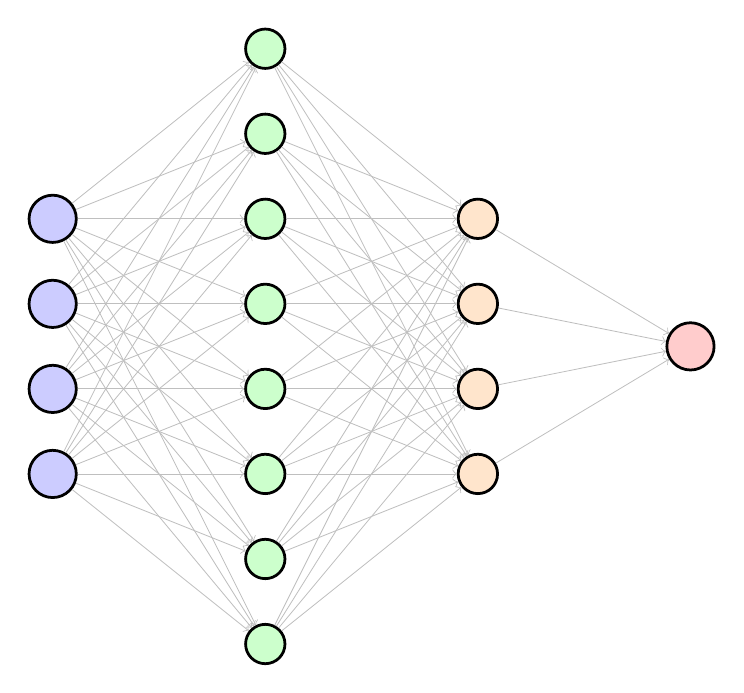
\begin{tikzpicture}[scale=0.9]
        % 定义神经元间距
        \def\spacing{1.2}
        
        % 输入层 - 4个神经元,关于横轴对称
        \node[circle, draw, minimum size=0.6cm, fill=blue!20, line width=1pt] (x1) at (0, -1.8) {};
        \node[circle, draw, minimum size=0.6cm, fill=blue!20, line width=1pt] (x2) at (0, -0.6) {};
        \node[circle, draw, minimum size=0.6cm, fill=blue!20, line width=1pt] (x3) at (0, 0.6) {};
        \node[circle, draw, minimum size=0.6cm, fill=blue!20, line width=1pt] (x4) at (0, 1.8) {};
        
        % 隐藏层1 - 8个神经元,关于横轴对称
        \node[circle, draw, minimum size=0.5cm, fill=green!20, line width=1pt] (h11) at (3, -4.2) {};
        \node[circle, draw, minimum size=0.5cm, fill=green!20, line width=1pt] (h12) at (3, -3.0) {};
        \node[circle, draw, minimum size=0.5cm, fill=green!20, line width=1pt] (h13) at (3, -1.8) {};
        \node[circle, draw, minimum size=0.5cm, fill=green!20, line width=1pt] (h14) at (3, -0.6) {};
        \node[circle, draw, minimum size=0.5cm, fill=green!20, line width=1pt] (h15) at (3, 0.6) {};
        \node[circle, draw, minimum size=0.5cm, fill=green!20, line width=1pt] (h16) at (3, 1.8) {};
        \node[circle, draw, minimum size=0.5cm, fill=green!20, line width=1pt] (h17) at (3, 3.0) {};
        \node[circle, draw, minimum size=0.5cm, fill=green!20, line width=1pt] (h18) at (3, 4.2) {};
        
        % 隐藏层2 - 4个神经元,关于横轴对称
        \node[circle, draw, minimum size=0.5cm, fill=orange!20, line width=1pt] (h21) at (6, -1.8) {};
        \node[circle, draw, minimum size=0.5cm, fill=orange!20, line width=1pt] (h22) at (6, -0.6) {};
        \node[circle, draw, minimum size=0.5cm, fill=orange!20, line width=1pt] (h23) at (6, 0.6) {};
        \node[circle, draw, minimum size=0.5cm, fill=orange!20, line width=1pt] (h24) at (6, 1.8) {};
        
        % 输出层 - 1个神经元,在横轴上
        \node[circle, draw, minimum size=0.6cm, fill=red!20, line width=1pt] (y) at (9, 0) {};
        
        % 输入层到隐藏层1的连接
        \foreach \i in {1,...,4}
            \foreach \j in {1,...,8}
                \draw[->, gray!50, line width=0.3pt] (x\i) -- (h1\j);
        
        % 隐藏层1到隐藏层2的连接
        \foreach \i in {1,...,8}
            \foreach \j in {1,...,4}
                \draw[->, gray!50, line width=0.3pt] (h1\i) -- (h2\j);
        
        % 隐藏层2到输出层的连接
        \foreach \i in {1,...,4}
            \draw[->, gray!50, line width=0.3pt] (h2\i) -- (y);
        \end{tikzpicture}
        
        \vfill
        \vspace{2cm}
        {\normalsize #5}
        \vspace{1.5cm}
    \end{center}
    \newpage
}



% 页眉页脚设置
\pagestyle{fancy}
\fancyhf{}
\fancyhead[L]{\leftmark}
\fancyhead[R]{\thepage}
\fancyfoot[C]{\small AI/LLM 基础教程}
\renewcommand{\headrulewidth}{0.3pt}
\renewcommand{\footrulewidth}{0.3pt}

\title{AI/LLM 基础教程}
\author{孙豪 \\ 中国人民大学}
\date{\today}

\newtheorem{definition}{定义}[section]
\newtheorem{theorem}{定理}[section]
\newtheorem{proposition}{命题}[section]
\newtheorem{example}{例}[section]
\newtheorem{remark}{注}[section]

\begin{document}

% 封面
\makecover{AI/LLM 基础教程}{数学基础 · Python 编程 · 机器学习 · 深度学习 · 大语言模型}{从基础理论到前沿应用,系统掌握人工智能和大语言模型核心技术}{}{孙豪 \quad 中国人民大学}

\newpage

\section*{引言}

欢迎阅读《AI/LLM 基础教程》!

本教程旨在为读者提供人工智能和大语言模型领域的系统性基础知识,涵盖从数学基础到前沿应用的完整知识体系。本教程包括以下六个核心部分:

\begin{itemize}
    \item \textbf{数学基础}:线性代数、概率论、优化理论、信息论、图论等核心数学工具
    \item \textbf{Python 编程基础}:Python 语法、NumPy 数值计算、Pandas 数据处理
    \item \textbf{机器学习}:监督学习、无监督学习、强化学习、特征工程、模型评估
    \item \textbf{深度学习}:神经网络、CNN、RNN、Transformer、优化技术
    \item \textbf{大语言模型基础}:Transformer 架构、注意力机制、预训练微调、提示工程、RAG
    \item \textbf{大语言模型先进技术}:参数高效微调、推理加速、模型部署、评估方法
\end{itemize}

\textbf{教程定位与使用建议}:

本教程采用\textbf{提纲挈领}的方式组织内容,重点在于构建知识框架、阐明核心概念和基本原理,而非详尽展开每一个技术细节。读者在学习过程中如遇到不理解的概念或需要更深入的细节,建议:

\begin{itemize}
    \item \textbf{查阅相关资料}:利用传统搜索引擎查找相关论文、技术文档和教程
    \item \textbf{使用AI工具}:借助现代AI搜索引擎和对话系统(如ChatGPT、Claude等)进行交互式学习,这些工具能够提供即时的解释和示例
    \item \textbf{实践验证}:通过编写代码、运行实验来验证和理解所学知识
\end{itemize}

\textbf{重要说明}:

\begin{itemize}
    \item \textbf{技术快速迭代}:大语言模型领域发展迅速,新技术、新方法不断涌现。本教程涵盖当前主流的基础理论和技术,但无法涵盖所有最新进展。读者应保持对前沿研究的关注。
    \item \textbf{持续学习的重要性}:完成本教程的学习后,建议读者:
    \begin{itemize}
        \item 持续关注最新的研究论文和技术博客
        \item 积极参与开源项目,在实践中掌握最新技术
        \item 关注行业动态,了解技术在实际应用中的发展
        \item 建立知识更新机制,保持与领域发展同步
    \end{itemize}
    \item \textbf{理论与实践并重}:本教程提供了理论基础和代码示例,但真正的掌握需要通过实际项目来巩固和深化。建议读者在学习过程中同步进行编程实践。
    \item \textbf{培养批判性思维}:在学习过程中,应保持批判性思维,深入理解技术的原理、适用场景和局限性,避免盲目使用。
\end{itemize}

希望本教程能够为您的 AI/LLM 学习之旅打下坚实的基础,并激发您继续深入探索的兴趣!

\newpage

% 优化目录格式:显示三层目录(section, subsection, subsubsection)
\setcounter{tocdepth}{3}
\tableofcontents
\newpage

% 开始导入各个部分的内容
% 注意:需要跳过各个文件的封面、标题和目录部分

% ========== 第一部分:数学基础 ==========
\newpage
\part{第一部分:数学基础}
\setcounter{section}{0}

\input{Math_content.tex}

% ========== 第二部分:Python 编程基础 ==========
\newpage
\part{第二部分:Python 编程基础}
\setcounter{section}{0}

\input{python_content.tex}

% ========== 第三部分:机器学习 ==========
\newpage
\part{第三部分:机器学习}
\setcounter{section}{0}

\section{引言}

机器学习(Machine Learning, ML)是人工智能的核心分支,通过从数据中自动学习模式和规律,使计算机系统能够完成特定任务而无需显式编程。机器学习在图像识别、自然语言处理、推荐系统、医疗诊断、金融风控等领域取得了显著成功。

\textbf{机器学习的独特价值}:
\begin{itemize}
    \item \textbf{处理高维特征}:能够处理包含数千甚至数万个特征的数据,自动发现重要特征
    \item \textbf{捕捉非线性关系}:通过非线性模型(如神经网络、核方法)捕捉数据中的复杂模式
    \item \textbf{自适应学习}:能够从新数据中持续学习,适应数据分布的变化
    \item \textbf{端到端学习}:直接从原始数据学习到最终输出,减少人工特征工程的需求
\end{itemize}

本文档系统性地介绍机器学习的核心理论、经典算法和实际应用,涵盖监督学习、无监督学习、强化学习等主要范式,以及特征工程、模型评估、集成学习等重要技术。

\section{机器学习基础}

机器学习根据学习方式可以分为三大类:监督学习、无监督学习和强化学习。每种范式适用于不同类型的问题和场景。

\subsection{监督学习}

\begin{definition}[监督学习]
监督学习(Supervised Learning)是从带标签的训练数据中学习一个映射函数 $f: \mathcal{X} \to \mathcal{Y}$,使得对于新的输入 $\mathbf{x} \in \mathcal{X}$,能够预测其标签 $y \in \mathcal{Y}$。

给定训练数据集 $\mathcal{D} = \{(\mathbf{x}_1, y_1), (\mathbf{x}_2, y_2), \ldots, (\mathbf{x}_n, y_n)\}$,其中 $\mathbf{x}_i \in \mathbb{R}^d$ 是特征向量,$y_i$ 是对应的标签,目标是学习函数 $f$ 使得 $f(\mathbf{x}_i) \approx y_i$。
\end{definition}

\textbf{通俗解释}:监督学习就像有老师指导的学习。老师提供大量"题目-答案"对(训练数据),学生(模型)通过学习这些例子,掌握解题方法,然后能够解答新的题目。

\subsubsection{分类问题}

分类问题的目标是预测离散的类别标签。根据类别数量,可以分为:
\begin{itemize}
    \item \textbf{二分类}:只有两个类别,如垃圾邮件分类(垃圾/正常)、疾病诊断(患病/健康)
    \item \textbf{多分类}:有多个类别,如图像分类(猫/狗/鸟等)、手写数字识别(0-9)
\end{itemize}

\textbf{典型应用}:
\begin{example}[垃圾邮件分类]
\textbf{问题}:自动识别邮件是否为垃圾邮件。

\textbf{数据}:
\begin{itemize}
    \item 特征:邮件内容中的词频、发件人信息、邮件标题等
    \item 标签:垃圾邮件(1)或正常邮件(0)
\end{itemize}

\textbf{方法}:使用朴素贝叶斯、逻辑回归或支持向量机等分类算法。

\textbf{实际应用}:Gmail 使用机器学习模型过滤垃圾邮件,准确率超过 99\%。
\end{example}

\subsubsection{回归问题}

回归问题的目标是预测连续的数值。

\textbf{典型应用}:
\begin{example}[房价预测]
\textbf{问题}:根据房屋特征预测房价。

\textbf{数据}:
\begin{itemize}
    \item 特征:面积、卧室数、位置、建造年份等
    \item 标签:房价(连续值)
\end{itemize}

\textbf{方法}:使用线性回归、决策树回归或神经网络等算法。

\textbf{实际应用}:Zillow 的 Zestimate 使用机器学习模型预测房价,帮助用户了解房产价值。
\end{example}

\subsubsection{监督学习的优势与局限性}

\textbf{优势}:
\begin{itemize}
    \item 有明确的优化目标(最小化预测误差)
    \item 可以使用大量标注数据进行训练
    \item 模型性能可以通过测试集准确评估
    \item 理论基础相对完善
\end{itemize}

\textbf{局限性}:
\begin{itemize}
    \item 需要大量标注数据,标注成本高
    \item 对标注质量要求高,错误标注会影响模型性能
    \item 难以处理标注数据稀缺的场景
    \item 模型可能过拟合训练数据
\end{itemize}

\subsection{无监督学习}

\begin{definition}[无监督学习]
无监督学习(Unsupervised Learning)是从无标签的数据中学习数据的内在结构和模式,不需要人工标注。

给定数据集 $\mathcal{D} = \{\mathbf{x}_1, \mathbf{x}_2, \ldots, \mathbf{x}_n\}$,其中只有特征向量,没有标签,目标是发现数据中的隐藏模式、结构或分布。
\end{definition}

\textbf{通俗解释}:无监督学习就像没有老师指导的自学。学生只能看到大量数据,需要自己发现其中的规律和模式,比如哪些数据相似、数据如何分组等。

\subsubsection{聚类}

聚类是将相似的数据点分组的过程。

\textbf{典型应用}:
\begin{example}[客户细分]
\textbf{问题}:根据客户的购买行为将其分为不同的群体。

\textbf{数据}:客户的购买历史、浏览记录、消费金额等特征(无标签)。

\textbf{方法}:使用 K-means、层次聚类等算法将客户分为若干群体。

\textbf{实际应用}:电商平台使用聚类分析进行客户细分,为不同群体提供个性化推荐和营销策略。
\end{example}

\subsubsection{降维}

降维是将高维数据映射到低维空间,保留主要信息。

\textbf{典型应用}:
\begin{example}[数据可视化]
\textbf{问题}:将高维数据(如 1000 维)可视化到 2D 或 3D 空间。

\textbf{方法}:使用 PCA(主成分分析)、t-SNE、UMAP 等降维算法。

\textbf{实际应用}:在生物信息学中,使用 t-SNE 将基因表达数据降维到 2D,可视化不同细胞类型的分布。
\end{example}

\subsubsection{无监督学习的优势与局限性}

\textbf{优势}:
\begin{itemize}
    \item 不需要标注数据,数据获取成本低
    \item 可以发现人类未预见的模式和结构
    \item 适用于探索性数据分析
    \item 可以作为监督学习的预处理步骤
\end{itemize}

\textbf{局限性}:
\begin{itemize}
    \item 没有明确的优化目标,评估困难
    \item 结果可能难以解释和验证
    \item 对参数选择敏感(如聚类数量)
    \item 可能发现无意义的模式
\end{itemize}

\subsection{强化学习}

\begin{definition}[强化学习]
强化学习(Reinforcement Learning, RL)是智能体(Agent)通过与环境的交互来学习最优策略,通过试错和奖励信号来指导学习过程。

强化学习问题可以建模为马尔可夫决策过程(MDP):$(\mathcal{S}, \mathcal{A}, \mathcal{P}, \mathcal{R}, \gamma)$,其中:
\begin{itemize}
    \item $\mathcal{S}$:状态空间
    \item $\mathcal{A}$:动作空间
    \item $\mathcal{P}$:状态转移概率
    \item $\mathcal{R}$:奖励函数
    \item $\gamma$:折扣因子
\end{itemize}

智能体的目标是学习策略 $\pi: \mathcal{S} \to \mathcal{A}$,最大化累积奖励:
$$R = \sum_{t=0}^{\infty} \gamma^t r_t$$
\end{definition}

\textbf{通俗解释}:强化学习就像训练宠物。宠物(智能体)做出动作(如坐下),主人(环境)给出奖励(如给食物)或惩罚(如不给食物)。通过反复尝试,宠物学会在什么情况下做什么动作能获得最多奖励。

\subsubsection{强化学习的核心概念}

\begin{itemize}
    \item \textbf{状态(State)}:环境在某个时刻的完整描述
    \item \textbf{动作(Action)}:智能体可以执行的操作
    \item \textbf{奖励(Reward)}:环境对智能体动作的反馈信号
    \item \textbf{策略(Policy)}:从状态到动作的映射
    \item \textbf{价值函数(Value Function)}:评估状态或动作的长期价值
\end{itemize}

\subsubsection{典型应用}

\begin{example}[游戏 AI]
\textbf{问题}:训练 AI 在游戏中达到人类或超人类水平。

\textbf{方法}:
\begin{itemize}
    \item Deep Q-Network (DQN):使用深度神经网络近似 Q 函数
    \item Policy Gradient:直接优化策略函数
    \item Actor-Critic:结合价值函数和策略梯度
\end{itemize}

\textbf{实际应用}:
\begin{itemize}
    \item \textbf{AlphaGo}:DeepMind 开发的围棋 AI,2016 年击败世界冠军李世石
    \item \textbf{AlphaStar}:在《星际争霸 II》中达到大师级水平
    \item \textbf{OpenAI Five}:在 Dota 2 中击败职业战队
\end{itemize}
\end{example}

\begin{example}[机器人控制]
\textbf{问题}:训练机器人完成复杂任务,如抓取物体、行走等。

\textbf{方法}:使用强化学习让机器人在仿真或真实环境中通过试错学习。

\textbf{实际应用}:Boston Dynamics 的机器人使用强化学习进行运动控制,实现复杂的平衡和移动能力。
\end{example}

\subsubsection{强化学习的优势与局限性}

\textbf{优势}:
\begin{itemize}
    \item 适用于序列决策问题
    \item 可以通过试错学习,不需要大量标注数据
    \item 能够学习长期策略
    \item 适用于动态环境
\end{itemize}

\textbf{局限性}:
\begin{itemize}
    \item 训练过程可能很慢,需要大量交互
    \item 奖励函数设计困难
    \item 探索与利用的平衡问题
    \item 安全性问题(在关键应用中)
\end{itemize}

\section{经典算法}

本节介绍机器学习中的经典算法,包括线性回归、决策树、随机森林和支持向量机。这些算法虽然相对简单,但在许多实际问题中仍然非常有效。

\subsection{线性回归}

线性回归是监督学习中最基础的算法之一,用于解决回归问题。

\begin{definition}[线性回归]
线性回归假设目标变量 $y$ 与特征向量 $\mathbf{x}$ 之间存在线性关系:
$$y = \mathbf{w}^T\mathbf{x} + b + \epsilon$$
其中 $\mathbf{w} \in \mathbb{R}^d$ 是权重向量,$b \in \mathbb{R}$ 是偏置项,$\epsilon$ 是误差项(通常假设 $\epsilon \sim \mathcal{N}(0, \sigma^2)$)。

给定训练数据 $\{(\mathbf{x}_i, y_i)\}_{i=1}^{n}$,线性回归的目标是找到参数 $\mathbf{w}$ 和 $b$,使得预测误差最小。
\end{definition}

\textbf{通俗解释}:线性回归就像用一条直线去拟合数据点。例如,用一条直线拟合"房屋面积-房价"的关系,直线的斜率和截距就是学到的参数。

\subsubsection{最小二乘法}

最常用的方法是最小二乘法(Least Squares),最小化平方误差:
$$L(\mathbf{w}, b) = \sum_{i=1}^{n} (y_i - (\mathbf{w}^T\mathbf{x}_i + b))^2$$

通过求导并令导数为零,可以得到闭式解:
$$\mathbf{w}^* = (\mathbf{X}^T\mathbf{X})^{-1}\mathbf{X}^T\mathbf{y}$$

其中 $\mathbf{X} \in \mathbb{R}^{n \times d}$ 是特征矩阵,$\mathbf{y} \in \mathbb{R}^n$ 是标签向量。

\subsubsection{正则化}

为了防止过拟合,可以加入正则化项:

\begin{itemize}
    \item \textbf{Ridge 回归($L_2$ 正则化)}:
    $$L_{\text{Ridge}} = \sum_{i=1}^{n} (y_i - \mathbf{w}^T\mathbf{x}_i)^2 + \lambda \|\mathbf{w}\|_2^2$$
    其中 $\lambda > 0$ 是正则化系数。Ridge 回归倾向于产生较小的权重。
    
    \item \textbf{Lasso 回归($L_1$ 正则化)}:
    $$L_{\text{Lasso}} = \sum_{i=1}^{n} (y_i - \mathbf{w}^T\mathbf{x}_i)^2 + \lambda \|\mathbf{w}\|_1$$
    Lasso 回归可以产生稀疏解(许多权重为 0),实现特征选择。
\end{itemize}

\subsubsection{应用场景}

\begin{example}[房价预测]
使用线性回归预测房价,特征包括面积、卧室数、位置等。Ridge 回归可以防止过拟合,Lasso 回归可以自动选择重要特征。
\end{example}

\begin{example}[股票价格预测]
使用历史价格、交易量等特征预测未来股价。虽然股价受多种因素影响,线性回归可以作为基准模型。
\end{example}

\subsubsection{优势与局限性}

\textbf{优势}:
\begin{itemize}
    \item 简单易懂,计算效率高
    \item 有闭式解,训练快速
    \item 可解释性强(权重表示特征重要性)
    \item 适合作为基准模型
\end{itemize}

\textbf{局限性}:
\begin{itemize}
    \item 只能捕捉线性关系
    \item 对异常值敏感
    \item 假设特征之间相互独立
    \item 需要特征工程(如多项式特征)来捕捉非线性
\end{itemize}

\subsection{决策树}

决策树是一种基于树结构的分类和回归算法,通过一系列规则进行决策。

\begin{definition}[决策树]
决策树(Decision Tree)是一个树形结构,其中:
\begin{itemize}
    \item 内部节点:表示特征测试
    \item 分支:表示测试结果
    \item 叶节点:表示类别标签或数值
\end{itemize}

从根节点到叶节点的路径对应一条决策规则。
\end{definition}

\textbf{通俗解释}:决策树就像医生诊断疾病的流程。先问"是否发烧?",如果"是"再问"是否咳嗽?",根据一系列问题的答案,最终得出诊断结果。

\subsubsection{构建决策树}

决策树的构建是一个递归过程:

\begin{algorithm}
\caption{构建决策树}
\begin{algorithmic}
\REQUIRE 训练数据集 $\mathcal{D}$,特征集 $\mathcal{F}$
\ENSURE 决策树 $T$
\IF{$\mathcal{D}$ 中所有样本属于同一类别}
    \STATE 返回叶节点,标记为该类别
\ELSIF{$\mathcal{F}$ 为空或 $\mathcal{D}$ 为空}
    \STATE 返回叶节点,标记为 $\mathcal{D}$ 中多数类
\ELSE
    \STATE 选择最优特征 $f^* = \arg\max_{f \in \mathcal{F}} \text{IG}(\mathcal{D}, f)$
    \STATE 为 $f^*$ 的每个可能值创建分支
    \FOR{每个分支}
        \STATE $D_v$ = $\mathcal{D}$ 中 $f^* = v$ 的样本子集
        \IF{$D_v$ 为空}
            \STATE 添加叶节点,标记为 $\mathcal{D}$ 中多数类
        \ELSE
            \STATE 递归构建子树:$\text{BuildTree}(D_v, \mathcal{F} \setminus \{f^*\})$
        \ENDIF
    \ENDFOR
\ENDIF
\end{algorithmic}
\end{algorithm}

\subsubsection{特征选择准则}

常用的特征选择准则包括:

\begin{itemize}
    \item \textbf{信息增益(Information Gain)}:
    $$\text{IG}(\mathcal{D}, f) = H(\mathcal{D}) - \sum_{v} \frac{|\mathcal{D}_v|}{|\mathcal{D}|} H(\mathcal{D}_v)$$
    其中 $H(\mathcal{D})$ 是数据集的熵。
    
    \item \textbf{基尼不纯度(Gini Impurity)}:
    $$G(\mathcal{D}) = 1 - \sum_{k} p_k^2$$
    其中 $p_k$ 是类别 $k$ 在数据集中的比例。
    
    \item \textbf{基尼增益}:
    $$\text{GiniGain}(\mathcal{D}, f) = G(\mathcal{D}) - \sum_{v} \frac{|\mathcal{D}_v|}{|\mathcal{D}|} G(\mathcal{D}_v)$$
\end{itemize}

\subsubsection{剪枝}

为了防止过拟合,需要对决策树进行剪枝:

\begin{itemize}
    \item \textbf{预剪枝}:在构建过程中提前停止(如限制树深度、最小样本数)
    \item \textbf{后剪枝}:构建完整树后,自底向上删除节点,用叶节点替代
\end{itemize}

\subsubsection{应用场景}

\begin{example}[医疗诊断]
使用决策树根据症状(发烧、咳嗽、头痛等)诊断疾病。决策树的可解释性使得医生可以理解诊断依据。
\end{example}

\begin{example}[信用评估]
银行使用决策树评估贷款申请人的信用风险,根据收入、工作年限、信用历史等特征做出决策。
\end{example}

\subsubsection{优势与局限性}

\textbf{优势}:
\begin{itemize}
    \item 可解释性强,决策过程清晰
    \item 可以处理数值和类别特征
    \item 不需要特征缩放
    \item 可以捕捉非线性关系
\end{itemize}

\textbf{局限性}:
\begin{itemize}
    \item 容易过拟合
    \item 对数据的小变化敏感(不稳定)
    \item 倾向于选择具有更多取值的特征
    \item 难以处理特征之间的交互
\end{itemize}

\subsection{随机森林}

随机森林(Random Forest)是决策树的集成方法,通过组合多个决策树来提高性能。

\begin{definition}[随机森林]
随机森林由 $B$ 棵决策树组成,每棵树在训练时:
\begin{enumerate}
    \item 使用自助采样(Bootstrap Sampling)从训练集中采样
    \item 在每个节点分裂时,随机选择 $k$ 个特征(通常 $k = \sqrt{d}$)进行考虑
\end{enumerate}

预测时,对于分类问题使用投票,对于回归问题使用平均。
\end{definition}

\textbf{通俗解释}:随机森林就像一群专家投票做决策。每个专家(决策树)根据自己的经验(不同的训练数据)给出意见,最终综合所有专家的意见做出决策。这样比单个专家更可靠。

\subsubsection{算法流程}

\begin{algorithm}
\caption{随机森林训练}
\begin{algorithmic}
\REQUIRE 训练数据集 $\mathcal{D}$,树的数量 $B$,特征采样数 $k$
\ENSURE 随机森林 $\{T_1, T_2, \ldots, T_B\}$
\FOR{$b = 1$ to $B$}
    \STATE 使用自助采样从 $\mathcal{D}$ 中采样得到 $\mathcal{D}_b$
    \STATE 使用 $\mathcal{D}_b$ 训练决策树 $T_b$,在每个节点随机选择 $k$ 个特征
\ENDFOR
\end{algorithmic}
\end{algorithm}

\subsubsection{随机性的作用}

随机森林通过两种随机性提高性能:
\begin{itemize}
    \item \textbf{样本随机性}:每棵树使用不同的训练样本(自助采样)
    \item \textbf{特征随机性}:每棵树在每个节点考虑不同的特征子集
\end{itemize}

这种随机性使得各棵树之间具有多样性,减少过拟合,提高泛化能力。

\subsubsection{应用场景}

\begin{example}[图像分类]
在 CIFAR-10 数据集上,随机森林可以作为基准模型,虽然不如深度学习模型,但训练速度快,可解释性强。
\end{example}

\begin{example}[特征重要性分析]
随机森林可以计算特征重要性,帮助理解哪些特征对预测最重要。这在特征工程和模型解释中很有价值。
\end{example}

\subsubsection{优势与局限性}

\textbf{优势}:
\begin{itemize}
    \item 性能通常优于单棵决策树
    \item 对过拟合有较强的抵抗力
    \item 可以处理高维特征
    \item 可以计算特征重要性
    \item 训练可以并行化
\end{itemize}

\textbf{局限性}:
\begin{itemize}
    \item 模型可解释性不如单棵决策树
    \item 需要更多内存和计算资源
    \item 对于某些问题,可能不如梯度提升方法(如 XGBoost)
\end{itemize}

\subsection{支持向量机}

支持向量机(Support Vector Machine, SVM)是一种强大的分类算法,基于最大间隔原理。

\begin{definition}[支持向量机]
对于线性可分的二分类问题,SVM 寻找一个超平面 $\mathbf{w}^T\mathbf{x} + b = 0$,使得两类样本之间的间隔(margin)最大。

间隔定义为两类样本到超平面的最小距离:
$$\text{margin} = \frac{2}{\|\mathbf{w}\|}$$

SVM 的优化目标是:
$$\min_{\mathbf{w}, b} \frac{1}{2}\|\mathbf{w}\|^2 \quad \text{s.t.} \quad y_i(\mathbf{w}^T\mathbf{x}_i + b) \geq 1, \forall i$$
\end{definition}

\textbf{通俗解释}:SVM 就像在两个群体之间画一条"最宽的路"。这条路要尽可能宽,同时要确保两边的群体都在路的正确一侧。支持向量就是那些"站在路边"的样本点。

\subsubsection{软间隔 SVM}

对于线性不可分的情况,引入松弛变量 $\xi_i$,允许一些样本分类错误:

$$\min_{\mathbf{w}, b, \boldsymbol{\xi}} \frac{1}{2}\|\mathbf{w}\|^2 + C\sum_{i=1}^{n}\xi_i$$

约束条件:
$$y_i(\mathbf{w}^T\mathbf{x}_i + b) \geq 1 - \xi_i, \quad \xi_i \geq 0$$

其中 $C > 0$ 是惩罚参数,控制对误分类的惩罚程度。

\subsubsection{核技巧}

对于非线性问题,使用核函数将数据映射到高维空间,在高维空间中线性可分:

$$K(\mathbf{x}_i, \mathbf{x}_j) = \phi(\mathbf{x}_i)^T\phi(\mathbf{x}_j)$$

常用的核函数包括:
\begin{itemize}
    \item \textbf{多项式核}:$K(\mathbf{x}_i, \mathbf{x}_j) = (\mathbf{x}_i^T\mathbf{x}_j + 1)^d$
    \item \textbf{径向基函数(RBF)核}:$K(\mathbf{x}_i, \mathbf{x}_j) = \exp(-\gamma\|\mathbf{x}_i - \mathbf{x}_j\|^2)$
    \item \textbf{Sigmoid 核}:$K(\mathbf{x}_i, \mathbf{x}_j) = \tanh(\alpha\mathbf{x}_i^T\mathbf{x}_j + c)$
\end{itemize}

\subsubsection{对偶形式}

SVM 的对偶形式为:
$$\max_{\boldsymbol{\alpha}} \sum_{i=1}^{n}\alpha_i - \frac{1}{2}\sum_{i,j}\alpha_i\alpha_j y_i y_j K(\mathbf{x}_i, \mathbf{x}_j)$$

约束条件:
$$\sum_{i=1}^{n}\alpha_i y_i = 0, \quad 0 \leq \alpha_i \leq C$$

对偶形式的优势:
\begin{itemize}
    \item 只需要计算核函数,不需要显式映射到高维空间
    \item 支持向量($\alpha_i > 0$)的数量通常远小于样本数
    \item 更容易扩展到大规模问题
\end{itemize}

\subsubsection{应用场景}

\begin{example}[文本分类]
SVM 在文本分类任务中表现优异,特别是在小样本情况下。使用 TF-IDF 特征和 RBF 核,可以在新闻分类、情感分析等任务中取得良好效果。
\end{example}

\begin{example}[图像分类]
在图像分类任务中,SVM 可以作为特征分类器。例如,使用 CNN 提取特征,然后用 SVM 进行分类,这在某些情况下比端到端的 CNN 更有效。
\end{example}

\subsubsection{优势与局限性}

\textbf{优势}:
\begin{itemize}
    \item 在中小规模数据集上表现优异
    \item 通过核函数可以处理非线性问题
    \item 理论基础完善(基于统计学习理论)
    \item 对过拟合有较好的控制
    \item 支持向量提供了模型的稀疏表示
\end{itemize}

\textbf{局限性}:
\begin{itemize}
    \item 对大规模数据集计算成本高
    \item 对特征缩放敏感
    \item 核函数和参数选择需要经验
    \item 可解释性不如决策树
    \item 概率输出需要额外处理(Platt scaling)
\end{itemize}

\section{特征工程}

特征工程是机器学习中至关重要的一环,好的特征可以显著提升模型性能。特征工程包括特征选择、特征变换和特征编码等。

\subsection{特征选择}

特征选择是从原始特征中选择最有用的特征子集,减少维度,提高模型性能和可解释性。

\subsubsection{过滤方法(Filter Methods)}

过滤方法基于特征的统计特性进行选择,独立于具体的学习算法:

\begin{itemize}
    \item \textbf{方差选择}:移除方差很小的特征(几乎不变的特征)
    \item \textbf{相关系数}:选择与目标变量相关性高的特征
    \item \textbf{互信息}:选择与目标变量互信息大的特征
    \item \textbf{卡方检验}:用于分类问题,检验特征与标签的独立性
\end{itemize}

\subsubsection{包装方法(Wrapper Methods)}

包装方法使用学习算法来评估特征子集:

\begin{itemize}
    \item \textbf{前向选择}:从空集开始,逐步添加最有用的特征
    \item \textbf{后向消除}:从完整特征集开始,逐步移除最无用的特征
    \item \textbf{递归特征消除(RFE)}:递归地移除最不重要的特征
\end{itemize}

\subsubsection{嵌入方法(Embedded Methods)}

嵌入方法在模型训练过程中进行特征选择:

\begin{itemize}
    \item \textbf{Lasso 回归}:$L_1$ 正则化自动产生稀疏解
    \item \textbf{决策树}:通过特征重要性进行选择
    \item \textbf{随机森林}:通过特征重要性排序
\end{itemize}

\subsection{特征变换}

特征变换是对特征进行数学变换,改变特征的分布或关系。

\subsubsection{标准化和归一化}

\begin{itemize}
    \item \textbf{标准化(Z-score)}:
    $$z = \frac{x - \mu}{\sigma}$$
    将特征转换为均值为 0、标准差为 1 的分布。
    
    \item \textbf{最小-最大归一化}:
    $$x' = \frac{x - x_{\min}}{x_{\max} - x_{\min}}$$
    将特征缩放到 $[0, 1]$ 区间。
    
    \item \textbf{Robust 缩放}:使用中位数和四分位距,对异常值更鲁棒。
\end{itemize}

\textbf{为什么需要特征缩放}:
\begin{itemize}
    \item 许多算法(如 SVM、K-means、神经网络)对特征尺度敏感
    \item 梯度下降算法在特征尺度不一致时收敛慢
    \item 距离-based 算法(如 KNN)受特征尺度影响大
\end{itemize}

\subsubsection{多项式特征}

通过创建特征的多项式组合来捕捉非线性关系:

$$(x_1, x_2) \to (x_1, x_2, x_1^2, x_1 x_2, x_2^2)$$

\textbf{应用场景}:线性回归无法捕捉非线性关系时,可以使用多项式特征。

\subsubsection{对数变换}

对偏态分布进行对数变换,使其更接近正态分布:

$$x' = \log(x + 1)$$

\textbf{应用场景}:处理价格、收入等右偏分布的数据。

\subsection{特征编码}

特征编码是将类别特征转换为数值特征的过程。

\subsubsection{独热编码(One-Hot Encoding)}

将类别特征转换为二进制向量:

\begin{example}
颜色特征:["红", "绿", "蓝"] $\to$ 
\begin{itemize}
    \item 红:$[1, 0, 0]$
    \item 绿:$[0, 1, 0]$
    \item 蓝:$[0, 0, 1]$
\end{itemize}
\end{example}

\textbf{优势}:不引入类别间的顺序关系。

\textbf{局限性}:类别数量多时会产生高维稀疏特征。

\subsubsection{标签编码(Label Encoding)}

将类别映射为整数:

\begin{example}
["低", "中", "高"] $\to$ [0, 1, 2]
\end{example}

\textbf{注意}:只适用于有序类别,否则会引入虚假的顺序关系。

\subsubsection{目标编码(Target Encoding)}

使用目标变量的统计量对类别进行编码:

$$x' = \frac{\sum_{i: x_i = x} y_i}{|\{i: x_i = x\}|}$$

即用该类别的平均目标值作为编码。

\textbf{优势}:可以捕捉类别与目标的关系。

\textbf{注意}:需要防止过拟合(如使用交叉验证)。

\section{模型评估与验证}

模型评估是机器学习流程中的关键步骤,用于衡量模型性能、选择最佳模型和防止过拟合。

\subsection{评估指标}

\subsubsection{分类问题指标}

\begin{itemize}
    \item \textbf{准确率(Accuracy)}:
    $$\text{Accuracy} = \frac{\text{正确预测数}}{\text{总样本数}}$$
    
    \item \textbf{精确率(Precision)}:
    $$\text{Precision} = \frac{\text{TP}}{\text{TP} + \text{FP}}$$
    预测为正例中真正为正例的比例。
    
    \item \textbf{召回率(Recall)}:
    $$\text{Recall} = \frac{\text{TP}}{\text{TP} + \text{FN}}$$
    真正例中被正确预测的比例。
    
    \item \textbf{F1 分数}:
    $$\text{F1} = \frac{2 \times \text{Precision} \times \text{Recall}}{\text{Precision} + \text{Recall}}$$
    精确率和召回率的调和平均。
    
    \item \textbf{ROC 曲线和 AUC}:ROC 曲线以假正例率为横轴,真正例率为纵轴。AUC(曲线下面积)衡量分类器的整体性能。
\end{itemize}

\subsubsection{回归问题指标}

\begin{itemize}
    \item \textbf{均方误差(MSE)}:
    $$\text{MSE} = \frac{1}{n}\sum_{i=1}^{n}(y_i - \hat{y}_i)^2$$
    
    \item \textbf{均方根误差(RMSE)}:
    $$\text{RMSE} = \sqrt{\text{MSE}}$$
    
    \item \textbf{平均绝对误差(MAE)}:
    $$\text{MAE} = \frac{1}{n}\sum_{i=1}^{n}|y_i - \hat{y}_i|$$
    
    \item \textbf{决定系数($R^2$)}:
    $$R^2 = 1 - \frac{\sum_{i=1}^{n}(y_i - \hat{y}_i)^2}{\sum_{i=1}^{n}(y_i - \bar{y})^2}$$
    衡量模型解释的方差比例。
\end{itemize}

\subsection{交叉验证}

交叉验证是评估模型泛化能力的重要方法。

\subsubsection{K 折交叉验证}

将数据集分为 $K$ 折,每次使用 $K-1$ 折训练,剩余 1 折测试,重复 $K$ 次:

\begin{algorithm}
\caption{K 折交叉验证}
\begin{algorithmic}
\REQUIRE 数据集 $\mathcal{D}$,折数 $K$,学习算法 $\mathcal{A}$
\ENSURE 平均性能指标
\STATE 将 $\mathcal{D}$ 随机分为 $K$ 折:$\mathcal{D}_1, \ldots, \mathcal{D}_K$
\FOR{$k = 1$ to $K$}
    \STATE 训练集:$\mathcal{D}_{\text{train}} = \mathcal{D} \setminus \mathcal{D}_k$
    \STATE 测试集:$\mathcal{D}_{\text{test}} = \mathcal{D}_k$
    \STATE 使用 $\mathcal{D}_{\text{train}}$ 训练模型 $M_k = \mathcal{A}(\mathcal{D}_{\text{train}})$
    \STATE 在 $\mathcal{D}_{\text{test}}$ 上评估性能 $s_k$
\ENDFOR
\RETURN $\bar{s} = \frac{1}{K}\sum_{k=1}^{K} s_k$
\end{algorithmic}
\end{algorithm}

\textbf{优势}:
\begin{itemize}
    \item 充分利用数据
    \item 提供性能估计的方差
    \item 减少对数据划分的依赖
\end{itemize}

\textbf{常见选择}:$K = 5$ 或 $K = 10$。

\subsubsection{留一法交叉验证(LOOCV)}

$K = n$ 的特殊情况,每次留一个样本作为测试集。计算成本高,但无偏估计。

\subsection{过拟合与欠拟合}

\begin{definition}[过拟合]
过拟合(Overfitting)是指模型在训练集上表现很好,但在测试集上表现较差的现象。模型过度学习了训练数据的噪声和细节,导致泛化能力差。
\end{definition}

\begin{definition}[欠拟合]
欠拟合(Underfitting)是指模型在训练集和测试集上都表现较差的现象。模型过于简单,无法捕捉数据中的基本模式。
\end{definition}

\textbf{通俗解释}:
\begin{itemize}
    \item \textbf{过拟合}:就像学生死记硬背了所有练习题,但遇到新题目就不会了
    \item \textbf{欠拟合}:就像学生只学了基础知识,连练习题都做不好
\end{itemize}

\subsubsection{识别过拟合和欠拟合}

\begin{itemize}
    \item \textbf{过拟合的迹象}:
    \begin{itemize}
        \item 训练误差很小,但验证误差很大
        \item 模型复杂度高(如深度很深的决策树)
        \item 训练集和验证集性能差距大
    \end{itemize}
    
    \item \textbf{欠拟合的迹象}:
    \begin{itemize}
        \item 训练误差和验证误差都很大
        \item 模型复杂度低(如线性模型处理非线性问题)
        \item 模型无法捕捉数据的基本模式
    \end{itemize}
\end{itemize}

\subsubsection{解决方法}

\textbf{解决过拟合}:
\begin{itemize}
    \item 增加训练数据
    \item 减少模型复杂度
    \item 正则化($L_1$、$L_2$)
    \item Dropout(神经网络)
    \item 早停(Early Stopping)
\end{itemize}

\textbf{解决欠拟合}:
\begin{itemize}
    \item 增加模型复杂度
    \item 增加特征
    \item 减少正则化
    \item 增加训练时间
\end{itemize}

\subsection{正则化}

正则化(Regularization)是防止过拟合的核心技术,通过在损失函数中添加惩罚项来约束模型参数,从而控制模型复杂度,提高泛化能力。

\begin{definition}[正则化]
正则化通过在原始损失函数中添加正则化项 $\Omega(\theta)$ 来约束模型参数:

$$L_{\text{reg}}(\theta) = L(\theta) + \lambda \Omega(\theta)$$

其中:
\begin{itemize}
    \item $L(\theta)$ 是原始损失函数(如均方误差、交叉熵)
    \item $\Omega(\theta)$ 是正则化项,衡量模型复杂度
    \item $\lambda > 0$ 是正则化系数,控制正则化强度
\end{itemize}
\end{definition}

\textbf{通俗解释}:正则化就像给模型"戴紧箍咒"。想象一个学生准备考试:
\begin{itemize}
    \item \textbf{没有正则化}:学生可能死记硬背所有题目,但遇到新题就不会了(过拟合)
    \item \textbf{有正则化}:限制学生只能记住重点知识,虽然训练题可能答得不够完美,但新题答得更好(泛化能力更强)
\end{itemize}

\textbf{正则化的核心思想}:
\begin{itemize}
    \item \textbf{奥卡姆剃刀原理}:在同样能解释数据的模型中,选择最简单的
    \item \textbf{约束参数空间}:限制模型参数的取值范围,防止参数过大
    \item \textbf{降低模型复杂度}:减少模型对训练数据的过度拟合
\end{itemize}

\subsubsection{$L_2$ 正则化(Ridge 回归)}

$L_2$ 正则化通过在损失函数中添加权重的平方和来约束参数。

\begin{definition}[$L_2$ 正则化]
对于线性模型 $f(\mathbf{x}) = \mathbf{w}^T\mathbf{x} + b$,$L_2$ 正则化的损失函数为:

$$L_{\text{Ridge}}(\mathbf{w}, b) = \sum_{i=1}^{n} (y_i - (\mathbf{w}^T\mathbf{x}_i + b))^2 + \lambda \|\mathbf{w}\|_2^2$$

其中 $\|\mathbf{w}\|_2^2 = \sum_{j=1}^{d} w_j^2$ 是权重的 $L_2$ 范数的平方。
\end{definition}

\textbf{数学推导}:

对权重求偏导并令其为零:

$$\frac{\partial L_{\text{Ridge}}}{\partial \mathbf{w}} = -2\mathbf{X}^T(\mathbf{y} - \mathbf{X}\mathbf{w}) + 2\lambda \mathbf{w} = 0$$

整理得到闭式解:

$$\mathbf{w}^* = (\mathbf{X}^T\mathbf{X} + \lambda \mathbf{I})^{-1}\mathbf{X}^T\mathbf{y}$$

其中 $\mathbf{I}$ 是单位矩阵。注意:$\lambda \mathbf{I}$ 使得矩阵 $(\mathbf{X}^T\mathbf{X} + \lambda \mathbf{I})$ 总是可逆的(即使 $\mathbf{X}^T\mathbf{X}$ 不可逆)。

\textbf{几何解释}:

$L_2$ 正则化等价于在参数空间中寻找一个点,使得:
\begin{itemize}
    \item 该点尽可能接近最优解(最小化原始损失)
    \item 该点的 $L_2$ 范数尽可能小(参数尽可能接近原点)
\end{itemize}

这相当于在参数空间中寻找一个"平衡点",既拟合数据又保持参数较小。

\textbf{特点}:
\begin{itemize}
    \item \textbf{平滑收缩}:所有参数按比例缩小,不会完全变为零
    \item \textbf{数值稳定}:即使特征高度相关,也能得到稳定解
    \item \textbf{可解释性}:参数保持非零,便于解释特征重要性
\end{itemize}

\textbf{应用场景}:
\begin{itemize}
    \item 特征数量大于样本数量时(高维数据)
    \item 特征之间存在多重共线性时
    \item 需要所有特征都参与预测时
\end{itemize}

\subsubsection{$L_1$ 正则化(Lasso 回归)}

$L_1$ 正则化通过在损失函数中添加权重的绝对值之和来约束参数,能够产生稀疏解。

\begin{definition}[$L_1$ 正则化]
对于线性模型 $f(\mathbf{x}) = \mathbf{w}^T\mathbf{x} + b$,$L_1$ 正则化的损失函数为:

$$L_{\text{Lasso}}(\mathbf{w}, b) = \sum_{i=1}^{n} (y_i - (\mathbf{w}^T\mathbf{x}_i + b))^2 + \lambda \|\mathbf{w}\|_1$$

其中 $\|\mathbf{w}\|_1 = \sum_{j=1}^{d} |w_j|$ 是权重的 $L_1$ 范数。
\end{definition}

\textbf{几何解释}:

$L_1$ 正则化的约束区域是一个菱形(在二维空间中)或超立方体(在高维空间中)。由于约束区域的"尖角"特性,最优解往往落在坐标轴上,导致某些参数恰好为零。

\textbf{稀疏性原理}:

\begin{theorem}[$L_1$ 正则化的稀疏性]
当正则化系数 $\lambda$ 足够大时,$L_1$ 正则化会将某些权重精确地压缩到零,实现特征选择。
\end{theorem}

\textbf{为什么 $L_1$ 能产生稀疏解?}

考虑二维情况,损失函数的等高线和 $L_1$ 约束区域(菱形)的交点:
\begin{itemize}
    \item $L_2$ 约束(圆形):等高线与圆的切点通常不在坐标轴上
    \item $L_1$ 约束(菱形):等高线与菱形的切点很可能在菱形的顶点(坐标轴上),使得某个参数为零
\end{itemize}

\textbf{特点}:
\begin{itemize}
    \item \textbf{特征选择}:自动将不重要的特征权重置为零
    \item \textbf{稀疏解}:产生稀疏的权重向量,模型更简洁
    \item \textbf{可解释性}:只保留重要特征,便于理解模型
    \item \textbf{计算挑战}:损失函数在零点不可导,需要特殊优化方法(如坐标下降、次梯度方法)
\end{itemize}

\textbf{应用场景}:
\begin{itemize}
    \item 特征数量远大于样本数量时
    \item 需要自动特征选择时
    \item 希望模型更简洁、可解释时
    \item 特征之间存在冗余时
\end{itemize}

\subsubsection{Elastic Net}

Elastic Net 结合了 $L_1$ 和 $L_2$ 正则化的优点,既能产生稀疏解,又能处理特征间的相关性。

\begin{definition}[Elastic Net]
Elastic Net 的正则化项是 $L_1$ 和 $L_2$ 正则化的线性组合:

$$L_{\text{Elastic Net}}(\mathbf{w}, b) = \sum_{i=1}^{n} (y_i - (\mathbf{w}^T\mathbf{x}_i + b))^2 + \lambda_1 \|\mathbf{w}\|_1 + \lambda_2 \|\mathbf{w}\|_2^2$$

通常写成:
$$L_{\text{Elastic Net}}(\mathbf{w}, b) = \sum_{i=1}^{n} (y_i - (\mathbf{w}^T\mathbf{x}_i + b))^2 + \lambda \left(\alpha \|\mathbf{w}\|_1 + (1-\alpha) \|\mathbf{w}\|_2^2\right)$$

其中 $\alpha \in [0, 1]$ 控制 $L_1$ 和 $L_2$ 的混合比例。
\end{definition}

\textbf{优势}:
\begin{itemize}
    \item \textbf{结合优点}:既有 $L_1$ 的稀疏性,又有 $L_2$ 的稳定性
    \item \textbf{处理相关性}:当特征高度相关时,$L_1$ 可能随机选择一个,而 Elastic Net 倾向于选择一组相关特征
    \item \textbf{灵活性}:通过调整 $\alpha$ 在稀疏性和稳定性之间权衡
\end{itemize}

\textbf{应用场景}:
\begin{itemize}
    \item 特征数量大于样本数量
    \item 特征之间存在高度相关性
    \item 需要特征选择但也要保持模型稳定性
\end{itemize}

\subsubsection{权重衰减(Weight Decay)}

在深度学习中,$L_2$ 正则化通常被称为权重衰减(Weight Decay)。

\begin{definition}[权重衰减]
在梯度下降更新中,权重衰减等价于在每次更新时对权重进行缩放:

$$\mathbf{w}_{t+1} = \mathbf{w}_t - \eta \nabla_\mathbf{w} L(\mathbf{w}_t) - \eta \lambda \mathbf{w}_t = (1 - \eta \lambda) \mathbf{w}_t - \eta \nabla_\mathbf{w} L(\mathbf{w}_t)$$

其中 $\eta$ 是学习率,$\lambda$ 是权重衰减系数。
\end{definition}

\textbf{通俗解释}:权重衰减就像"记忆衰减"。每次更新参数时,不仅根据梯度调整,还会让参数"忘记"一部分(乘以小于1的因子),防止参数变得过大。

\textbf{在优化器中的应用}:

大多数现代优化器(如 Adam、SGD)都支持权重衰减:

\begin{itemize}
    \item \textbf{SGD with Weight Decay}:
    $$\mathbf{w}_{t+1} = \mathbf{w}_t - \eta (\nabla_\mathbf{w} L(\mathbf{w}_t) + \lambda \mathbf{w}_t)$$
    
    \item \textbf{Adam with Weight Decay}:在 Adam 的更新公式中加入权重衰减项
\end{itemize}

\textbf{注意事项}:
\begin{itemize}
    \item 权重衰减通常不应用于偏置项 $b$
    \item 权重衰减系数需要与学习率一起调整
    \item 过大的权重衰减可能导致欠拟合
\end{itemize}

\subsubsection{早停(Early Stopping)}

早停是一种简单有效的正则化方法,通过在验证集性能不再提升时停止训练来防止过拟合。

\begin{definition}[早停]
早停算法:
\begin{enumerate}
    \item 将数据集分为训练集和验证集
    \item 在训练过程中,定期在验证集上评估模型性能
    \item 如果验证集性能在 $k$ 个epoch内没有提升,则停止训练
    \item 返回验证集性能最好的模型参数
\end{enumerate}
\end{definition}

\textbf{为什么早停有效?}

\begin{itemize}
    \item \textbf{防止过训练}:训练时间过长时,模型可能开始记忆训练数据的噪声
    \item \textbf{自动选择最优模型}:在验证集上性能最好的模型通常泛化能力最强
    \item \textbf{计算效率}:不需要训练到收敛,节省计算资源
\end{itemize}

\textbf{实现细节}:
\begin{itemize}
    \item \textbf{耐心(Patience)}:允许验证集性能不提升的epoch数
    \item \textbf{最小改善(Min Delta)}:验证集性能的最小改善阈值
    \item \textbf{恢复最佳权重}:训练结束后恢复验证集上表现最好的权重
\end{itemize}

\textbf{应用场景}:
\begin{itemize}
    \item 深度学习模型训练
    \item 训练时间有限时
    \item 需要自动选择最优模型时
\end{itemize}

\subsubsection{数据增强(Data Augmentation)}

数据增强通过人工增加训练数据来防止过拟合,是一种隐式的正则化方法。

\begin{definition}[数据增强]
数据增强通过对原始数据进行变换生成新的训练样本,常见变换包括:
\begin{itemize}
    \item \textbf{图像}:旋转、翻转、缩放、裁剪、颜色变换、噪声添加
    \item \textbf{文本}:同义词替换、回译、随机删除、随机插入
    \item \textbf{音频}:时间拉伸、音调变换、添加噪声
\end{itemize}
\end{definition}

\textbf{为什么数据增强有效?}

\begin{itemize}
    \item \textbf{增加数据多样性}:让模型看到更多数据变体,提高鲁棒性
    \item \textbf{隐式正则化}:通过增加数据量,间接减少过拟合风险
    \item \textbf{提高泛化能力}:模型学习到更通用的特征,而不是记忆特定样本
\end{itemize}

\textbf{应用场景}:
\begin{itemize}
    \item 训练数据有限时
    \item 需要提高模型鲁棒性时
    \item 计算机视觉、自然语言处理等领域
\end{itemize}

\subsubsection{正则化方法对比}

\begin{table}[h]
\centering
\begin{tabular}{p{3cm}p{4cm}p{4cm}p{4cm}}
\toprule
\textbf{方法} & \textbf{优点} & \textbf{缺点} & \textbf{适用场景} \\
\midrule
$L_2$ 正则化 & 数值稳定、平滑收缩 & 不产生稀疏解 & 特征相关、需要所有特征 \\
\midrule
$L_1$ 正则化 & 特征选择、稀疏解 & 数值不稳定、优化困难 & 高维数据、特征选择 \\
\midrule
Elastic Net & 结合两者优点 & 需要调两个超参数 & 特征相关且需要选择 \\
\midrule
权重衰减 & 简单有效、广泛支持 & 需要调超参数 & 深度学习模型 \\
\midrule
早停 & 简单、自动选择模型 & 需要验证集 & 训练时间可控 \\
\midrule
数据增强 & 提高鲁棒性 & 需要领域知识 & 数据有限时 \\
\bottomrule
\end{tabular}
\caption{正则化方法对比}
\end{table}

\subsubsection{正则化系数选择}

正则化系数 $\lambda$ 的选择至关重要,通常通过交叉验证来确定。

\textbf{选择方法}:
\begin{itemize}
    \item \textbf{网格搜索}:在预定义的范围内搜索最优 $\lambda$
    \item \textbf{随机搜索}:随机采样 $\lambda$ 值
    \item \textbf{贝叶斯优化}:使用更智能的搜索策略
    \item \textbf{学习曲线}:观察不同 $\lambda$ 下的训练/验证误差
\end{itemize}

\textbf{经验法则}:
\begin{itemize}
    \item $\lambda$ 太小:正则化效果弱,可能过拟合
    \item $\lambda$ 太大:正则化过强,可能欠拟合
    \item 通常从 $10^{-4}$ 到 $10^2$ 的范围开始搜索
\end{itemize}

\subsubsection{正则化在深度学习中的应用}

在深度学习中,正则化技术更加多样:

\begin{itemize}
    \item \textbf{Dropout}:随机丢弃神经元(详见深度学习部分)
    \item \textbf{Batch Normalization}:归一化层输入,具有隐式正则化效果
    \item \textbf{权重衰减}:$L_2$ 正则化在深度学习中的实现
    \item \textbf{标签平滑}:防止模型过度自信
    \item \textbf{噪声注入}:在输入或隐藏层添加噪声
\end{itemize}

这些技术将在深度学习部分详细讨论。

\subsection{偏差-方差权衡}

\begin{definition}[偏差和方差]
\begin{itemize}
    \item \textbf{偏差(Bias)}:模型的期望预测与真实值的差异,衡量模型的拟合能力
    \item \textbf{方差(Variance)}:模型在不同训练集上预测的差异,衡量模型的稳定性
\end{itemize}

总误差可以分解为:
$$\text{Error} = \text{Bias}^2 + \text{Variance} + \text{Irreducible Error}$$
\end{definition}

\textbf{通俗解释}:
\begin{itemize}
    \item \textbf{高偏差}:模型太简单,无法捕捉数据模式(欠拟合)
    \item \textbf{高方差}:模型太复杂,对训练数据的小变化敏感(过拟合)
\end{itemize}

\subsubsection{偏差-方差权衡}

\begin{itemize}
    \item \textbf{简单模型}(如线性回归):
    \begin{itemize}
        \item 高偏差,低方差
        \item 可能欠拟合
    \end{itemize}
    
    \item \textbf{复杂模型}(如深度神经网络):
    \begin{itemize}
        \item 低偏差,高方差
        \item 可能过拟合
    \end{itemize}
    
    \item \textbf{理想模型}:
    \begin{itemize}
        \item 低偏差,低方差
        \item 需要合适的模型复杂度和正则化
    \end{itemize}
\end{itemize}

\section{集成学习方法}

集成学习通过组合多个基学习器来提高预测性能,是机器学习中的重要技术。

\subsection{Bagging}

Bagging(Bootstrap Aggregating)通过训练多个模型并平均预测结果来减少方差。

\begin{definition}[Bagging]
Bagging 算法:
\begin{enumerate}
    \item 使用自助采样从训练集中生成 $B$ 个不同的训练集
    \item 在每个训练集上训练一个基学习器
    \item 对于分类问题使用投票,对于回归问题使用平均
\end{enumerate}
\end{definition}

\textbf{通俗解释}:Bagging 就像多个专家独立给出意见,然后综合所有意见做决策。每个专家看到的数据略有不同,但综合起来更可靠。

\subsubsection{随机森林}

随机森林是 Bagging 的特例,基学习器是决策树,并在特征选择时引入随机性。

\subsubsection{优势与局限性}

\textbf{优势}:
\begin{itemize}
    \item 减少方差,提高泛化能力
    \item 可以并行训练
    \item 对过拟合有抵抗力
\end{itemize}

\textbf{局限性}:
\begin{itemize}
    \item 不能减少偏差
    \item 需要足够的计算资源
\end{itemize}

\subsection{Boosting}

Boosting 通过顺序训练多个弱学习器,每个学习器关注前一个学习器的错误。

\begin{definition}[Boosting]
Boosting 算法:
\begin{enumerate}
    \item 初始化样本权重
    \item 对于 $t = 1, \ldots, T$:
    \begin{itemize}
        \item 使用当前权重训练弱学习器 $h_t$
        \item 计算 $h_t$ 的误差
        \item 更新样本权重(增加错误样本的权重)
        \item 计算 $h_t$ 的权重 $\alpha_t$
    \end{itemize}
    \item 最终预测:$H(\mathbf{x}) = \sum_{t=1}^{T} \alpha_t h_t(\mathbf{x})$
\end{enumerate}
\end{definition}

\textbf{通俗解释}:Boosting 就像学生做错题后,老师重点讲解错题,学生反复练习直到掌握。每个弱学习器专注于前一个学习器的薄弱环节。

\subsubsection{AdaBoost}

AdaBoost(Adaptive Boosting)是经典的 Boosting 算法:

\begin{algorithm}
\caption{AdaBoost}
\begin{algorithmic}
\REQUIRE 训练集 $\mathcal{D} = \{(\mathbf{x}_i, y_i)\}_{i=1}^{n}$,弱学习器 $\mathcal{A}$,迭代次数 $T$
\ENSURE 集成模型 $H$
\STATE 初始化样本权重:$w_i^{(1)} = 1/n, \forall i$
\FOR{$t = 1$ to $T$}
    \STATE 使用权重 $\mathbf{w}^{(t)}$ 训练弱学习器:$h_t = \mathcal{A}(\mathcal{D}, \mathbf{w}^{(t)})$
    \STATE 计算加权误差:$\epsilon_t = \sum_{i: h_t(\mathbf{x}_i) \neq y_i} w_i^{(t)}$
    \STATE 计算学习器权重:$\alpha_t = \frac{1}{2}\ln\left(\frac{1-\epsilon_t}{\epsilon_t}\right)$
    \STATE 更新样本权重:$w_i^{(t+1)} = \frac{w_i^{(t)}}{Z_t} \exp(-\alpha_t y_i h_t(\mathbf{x}_i))$
\ENDFOR
\RETURN $H(\mathbf{x}) = \text{sign}\left(\sum_{t=1}^{T} \alpha_t h_t(\mathbf{x})\right)$
\end{algorithmic}
\end{algorithm}

\subsubsection{梯度提升}

梯度提升(Gradient Boosting)将 Boosting 视为优化问题,使用梯度下降来最小化损失函数。

\textbf{核心思想}:每个新学习器拟合前一个模型的负梯度(残差)。

\subsubsection{XGBoost 和 LightGBM}

\begin{itemize}
    \item \textbf{XGBoost}:优化的梯度提升实现,支持并行计算、正则化、处理缺失值
    \item \textbf{LightGBM}:更快的梯度提升实现,使用基于直方图的算法和 Leaf-wise 树生长策略
\end{itemize}

\textbf{应用场景}:在 Kaggle 等数据科学竞赛中,XGBoost 和 LightGBM 经常是获胜方案的核心组件。

\subsubsection{优势与局限性}

\textbf{优势}:
\begin{itemize}
    \item 通常比单个模型性能更好
    \item 可以减少偏差和方差
    \item 可以处理各种类型的数据
\end{itemize}

\textbf{局限性}:
\begin{itemize}
    \item 训练时间较长(顺序训练)
    \item 对异常值敏感
    \item 可解释性较差
\end{itemize}

\subsection{Stacking}

Stacking(堆叠)使用元学习器来组合多个基学习器的预测。

\begin{definition}[Stacking]
Stacking 算法:
\begin{enumerate}
    \item 使用交叉验证训练多个基学习器
    \item 使用基学习器的预测作为特征,训练元学习器
    \item 最终预测使用元学习器
\end{enumerate}
\end{definition}

\textbf{通俗解释}:Stacking 就像有一个"超级裁判",它不直接看原始数据,而是看各个"专家"(基学习器)的意见,然后综合这些意见做出最终判断。

\subsubsection{算法流程}

\begin{algorithm}
\caption{Stacking}
\begin{algorithmic}
\REQUIRE 训练集 $\mathcal{D}$,基学习器 $\{\mathcal{A}_1, \ldots, \mathcal{A}_M\}$,元学习器 $\mathcal{A}_{\text{meta}}$
\ENSURE 集成模型
\STATE 使用 K 折交叉验证训练基学习器
\FOR{$m = 1$ to $M$}
    \FOR{每折 $k$}
        \STATE 在折 $k$ 的训练集上训练 $h_{m,k}$
        \STATE 在折 $k$ 的验证集上生成预测 $p_{m,k}$
    \ENDFOR
    \STATE 基学习器 $m$ 的完整预测:$\mathbf{p}_m = [p_{m,1}, \ldots, p_{m,K}]$
\ENDFOR
\STATE 使用 $\{(\mathbf{p}_1, \ldots, \mathbf{p}_M), \mathbf{y}\}$ 训练元学习器
\RETURN 集成模型(基学习器 + 元学习器)
\end{algorithmic}
\end{algorithm}

\subsubsection{优势与局限性}

\textbf{优势}:
\begin{itemize}
    \item 可以捕捉基学习器之间的互补性
    \item 通常性能优于单个模型
    \item 灵活性高,可以使用不同类型的基学习器
\end{itemize}

\textbf{局限性}:
\begin{itemize}
    \item 计算成本高
    \item 需要仔细设计,避免过拟合
    \item 可解释性差
\end{itemize}

\section{在线学习与增量学习}

在线学习和增量学习使模型能够从新数据中持续学习,适应数据分布的变化。

\subsection{在线学习}

\begin{definition}[在线学习]
在线学习(Online Learning)是一种学习范式,模型逐个处理样本,每处理一个样本就更新模型参数,不需要存储所有历史数据。

给定数据流 $\{(\mathbf{x}_1, y_1), (\mathbf{x}_2, y_2), \ldots\}$,在线学习算法在时刻 $t$:
\begin{enumerate}
    \item 接收样本 $(\mathbf{x}_t, y_t)$
    \item 使用当前模型 $f_t$ 进行预测
    \item 根据预测误差更新模型:$f_{t+1} = \text{Update}(f_t, (\mathbf{x}_t, y_t))$
\end{enumerate}
\end{definition}

\textbf{通俗解释}:在线学习就像实时学习,每来一个新例子就立即学习,不需要等所有数据都收集完。就像学生每做一道题就立即知道答案并学习,而不是等所有题目做完再统一学习。

\subsubsection{在线梯度下降}

在线梯度下降是随机梯度下降的在线版本:

$$\mathbf{w}_{t+1} = \mathbf{w}_t - \eta_t \nabla_{\mathbf{w}} \ell(f(\mathbf{x}_t; \mathbf{w}_t), y_t)$$

其中 $\eta_t$ 是学习率,通常随时间衰减。

\subsubsection{应用场景}

\begin{example}[推荐系统]
在线推荐系统需要实时响应用户行为,根据用户的实时反馈更新推荐模型。例如,用户点击了某个商品,系统立即更新该用户的兴趣模型。
\end{example}

\begin{example}[广告投放]
在线广告系统需要根据实时点击率调整广告投放策略,快速适应市场变化。
\end{example}

\subsubsection{优势与局限性}

\textbf{优势}:
\begin{itemize}
    \item 内存效率高(不需要存储所有数据)
    \item 可以快速适应数据分布变化
    \item 适合大规模数据流
    \item 可以实时更新模型
\end{itemize}

\textbf{局限性}:
\begin{itemize}
    \item 对异常值敏感
    \item 可能遗忘历史信息
    \item 需要仔细设计学习率
    \item 难以评估模型性能
\end{itemize}

\subsection{增量学习}

\begin{definition}[增量学习]
增量学习(Incremental Learning)是模型在已有知识的基础上,从新数据中学习新知识,同时保留或整合旧知识的过程。

与在线学习的区别:增量学习通常处理批量新数据,并且需要处理"灾难性遗忘"问题。
\end{definition}

\textbf{通俗解释}:增量学习就像人类学习新知识。学习新内容时,不会完全忘记旧知识,而是将新旧知识整合在一起。但机器学习模型容易"遗忘"旧知识,需要特殊技术来解决。

\subsubsection{灾难性遗忘}

灾难性遗忘(Catastrophic Forgetting)是指模型在学习新任务时,会大幅降低在旧任务上的性能。

\textbf{原因}:神经网络参数在训练新任务时被更新,可能破坏对旧任务的记忆。

\subsubsection{解决方法}

\begin{itemize}
    \item \textbf{弹性权重巩固(EWC)}:在更新参数时,对重要参数施加惩罚,防止大幅改变
    \item \textbf{渐进式神经网络}:为每个任务添加新的网络分支,保留旧网络不变
    \item \textbf{回放机制}:存储部分旧数据,与新数据一起训练
    \item \textbf{知识蒸馏}:使用旧模型指导新模型学习
\end{itemize}

\subsubsection{应用场景}

\begin{example}[持续学习系统]
智能助手需要不断学习新技能,但不能忘记已有技能。例如,学习新语言时不能忘记已掌握的语言。
\end{example}

\begin{example}[个性化推荐]
推荐系统需要适应用户兴趣的变化,同时保留对用户长期偏好的理解。
\end{example}

\section{总结}

本文档系统性地介绍了机器学习的核心理论与应用,包括:

\begin{itemize}
    \item \textbf{机器学习基础}:监督学习、无监督学习和强化学习三大范式,每种范式适用于不同类型的问题
    \item \textbf{经典算法}:线性回归、决策树、随机森林和支持向量机等基础算法,虽然简单但在许多场景中仍然有效
    \item \textbf{特征工程}:特征选择、变换和编码等技术,是提升模型性能的关键
    \item \textbf{模型评估}:交叉验证、过拟合/欠拟合识别、偏差-方差权衡等评估技术
    \item \textbf{集成学习}:Bagging、Boosting 和 Stacking 等方法,通过组合多个模型提高性能
    \item \textbf{在线与增量学习}:使模型能够从新数据中持续学习,适应动态环境
\end{itemize}

\textbf{机器学习的核心价值}:
\begin{itemize}
    \item 能够从数据中自动学习模式,减少人工规则设计
    \item 可以处理高维、复杂的现实世界数据
    \item 通过持续学习适应环境变化
    \item 在多个领域取得了突破性进展
\end{itemize}

\textbf{未来发展方向}:
\begin{itemize}
    \item 自动化机器学习(AutoML):减少人工调参和特征工程
    \item 可解释性:提高模型的可解释性和可信度
    \item 持续学习:更好地处理数据分布变化和任务演化
    \item 小样本学习:在数据稀缺场景下仍能有效学习
    \item 联邦学习:在保护隐私的前提下进行分布式学习
\end{itemize}

机器学习作为人工智能的核心技术,将继续在各个领域发挥重要作用,推动技术进步和社会发展。



% ========== 第四部分:深度学习 ==========
\newpage
\part{第四部分:深度学习}
\setcounter{section}{0}

\input{DL_content.tex}

% ========== 第五部分:大语言模型基础 ==========
\newpage
\part{第五部分:大语言模型基础}
\setcounter{section}{0}

\input{LLM_content.tex}

% ========== 第六部分:大语言模型先进技术 ==========
\newpage
\part{第六部分:大语言模型先进技术}
\setcounter{section}{0}

\section{参数高效微调技术}

传统的全参数微调需要更新模型的所有参数,对于大模型来说成本极高。参数高效微调(Parameter-Efficient Fine-Tuning, PEFT)技术通过只更新少量参数就能达到接近全参数微调的效果,大幅降低了微调成本。

\subsection{LoRA (Low-Rank Adaptation)}

\textbf{概念解释}:LoRA 是 Microsoft 在 2021 年提出的参数高效微调方法。其核心思想是:对于预训练模型的权重矩阵 $\mathbf{W}$,不直接更新它,而是学习一个低秩分解的增量 $\Delta\mathbf{W}$,使得 $\mathbf{W} + \Delta\mathbf{W}$ 能够适应新任务。

\textbf{数学公式}:

对于原始权重矩阵 $\mathbf{W} \in \mathbb{R}^{d \times k}$,LoRA 将其更新分解为:
\begin{equation}
\mathbf{W}' = \mathbf{W} + \Delta\mathbf{W} = \mathbf{W} + \mathbf{B}\mathbf{A}
\end{equation}

其中:
\begin{itemize}
    \item $\mathbf{A} \in \mathbb{R}^{r \times k}$:低秩矩阵,随机初始化
    \item $\mathbf{B} \in \mathbb{R}^{d \times r}$:低秩矩阵,初始化为零
    \item $r \ll \min(d, k)$:秩(rank),通常 $r \in \{4, 8, 16, 32, 64\}$
\end{itemize}

在前向传播时:
\begin{equation}
\mathbf{h} = \mathbf{W}'\mathbf{x} = (\mathbf{W} + \mathbf{B}\mathbf{A})\mathbf{x} = \mathbf{W}\mathbf{x} + \mathbf{B}(\mathbf{A}\mathbf{x})
\end{equation}

\textbf{参数量对比}:
\begin{itemize}
    \item 全参数微调:$d \times k$ 个参数
    \item LoRA:$r \times (d + k)$ 个参数
    \item 参数减少比例:$\frac{r(d + k)}{dk} = r\left(\frac{1}{k} + \frac{1}{d}\right)$
\end{itemize}

当 $r = 8$,$d = 4096$,$k = 4096$ 时,参数量从 $16,777,216$ 减少到 $65,536$,减少了约 $256$ 倍。

\textbf{算法原理}:
\begin{algorithm}
\caption{LoRA 微调算法}
\begin{algorithmic}[1]
\REQUIRE 预训练模型权重 $\mathbf{W}$,训练数据 $\mathcal{D}$,秩 $r$,学习率 $\eta$
\ENSURE LoRA 权重 $\mathbf{A}$ 和 $\mathbf{B}$
\STATE 初始化 $\mathbf{A}$ 为随机小值,$\mathbf{B}$ 为零矩阵
\STATE 冻结原始权重 $\mathbf{W}$
\REPEAT
    \FOR{每个批次 $(\mathbf{x}, \mathbf{y}) \in \mathcal{D}$}
        \STATE 前向传播:$\mathbf{h} = \mathbf{W}\mathbf{x} + \mathbf{B}(\mathbf{A}\mathbf{x})$
        \STATE 计算损失:$\mathcal{L} = \text{loss}(\mathbf{h}, \mathbf{y})$
        \STATE 反向传播,只更新 $\mathbf{A}$ 和 $\mathbf{B}$
        \STATE $\mathbf{A} \leftarrow \mathbf{A} - \eta \nabla_{\mathbf{A}}\mathcal{L}$
        \STATE $\mathbf{B} \leftarrow \mathbf{B} - \eta \nabla_{\mathbf{B}}\mathcal{L}$
    \ENDFOR
\UNTIL{收敛}
\end{algorithmic}
\end{algorithm}

\textbf{代码实现}:

\begin{lstlisting}[caption=LoRA 从零实现]
import torch
import torch.nn as nn
import torch.nn.functional as F

class LoRALayer(nn.Module):
    """LoRA 层实现"""
    
    def __init__(self, in_features, out_features, rank=8, alpha=16, dropout=0.0):
        """
        参数:
            in_features: 输入特征维度
            out_features: 输出特征维度
            rank: LoRA 的秩
            alpha: 缩放因子,通常等于 rank
            dropout: Dropout 概率
        """
        super().__init__()
        self.rank = rank
        self.alpha = alpha
        self.scaling = alpha / rank
        
        # LoRA 矩阵 A 和 B
        self.lora_A = nn.Parameter(torch.randn(rank, in_features) * 0.02)
        self.lora_B = nn.Parameter(torch.zeros(out_features, rank))
        
        # Dropout
        self.dropout = nn.Dropout(dropout) if dropout > 0 else nn.Identity()
        
        # 原始权重(冻结)
        self.weight = None  # 将在外部设置
    
    def forward(self, x, weight):
        """
        前向传播
        
        参数:
            x: 输入张量 (batch_size, ..., in_features)
            weight: 原始权重矩阵 (out_features, in_features)
        """
        # 原始输出
        original_output = F.linear(x, weight)
        
        # LoRA 输出: B @ (A @ x)
        x_dropout = self.dropout(x)
        lora_output = F.linear(
            F.linear(x_dropout, self.lora_A),
            self.lora_B
        )
        
        # 缩放并相加
        return original_output + self.scaling * lora_output

class LoRALinear(nn.Module):
    """包装的 LoRA 线性层"""
    
    def __init__(self, linear_layer, rank=8, alpha=16, dropout=0.0):
        super().__init__()
        self.original = linear_layer
        self.lora = LoRALayer(
            linear_layer.in_features,
            linear_layer.out_features,
            rank,
            alpha,
            dropout
        )
        # 冻结原始权重
        for param in self.original.parameters():
            param.requires_grad = False
    
    def forward(self, x):
        return self.lora(x, self.original.weight)

# 使用示例
# 假设我们有一个预训练的线性层
pretrained_linear = nn.Linear(768, 3072)

# 包装为 LoRA 层
lora_linear = LoRALinear(pretrained_linear, rank=8, alpha=16)

# 前向传播
x = torch.randn(32, 768)  # batch_size=32
output = lora_linear(x)
print(f"输入形状: {x.shape}")
print(f"输出形状: {output.shape}")

# 检查可训练参数
total_params = sum(p.numel() for p in lora_linear.parameters() if p.requires_grad)
print(f"可训练参数数量: {total_params}")  # 8 * (768 + 3072) = 30720
print(f"原始参数数量: {pretrained_linear.weight.numel()}")  # 768 * 3072 = 2359296
print(f"参数减少比例: {pretrained_linear.weight.numel() / total_params:.2f}x")
\end{lstlisting}

\textbf{使用 PEFT 库实现}:

\begin{lstlisting}[caption=使用 Hugging Face PEFT 库]
from transformers import AutoModelForCausalLM, AutoTokenizer
from peft import LoraConfig, get_peft_model, TaskType

# 加载预训练模型
model_name = "meta-llama/Llama-2-7b-hf"  # 示例模型
model = AutoModelForCausalLM.from_pretrained(
    model_name,
    torch_dtype=torch.float16,
    device_map="auto"
)
tokenizer = AutoTokenizer.from_pretrained(model_name)

# 配置 LoRA
lora_config = LoraConfig(
    task_type=TaskType.CAUSAL_LM,
    r=8,  # rank
    lora_alpha=16,  # alpha
    lora_dropout=0.1,
    target_modules=["q_proj", "v_proj", "k_proj", "o_proj"],  # 目标模块
    bias="none"
)

# 应用 LoRA
model = get_peft_model(model, lora_config)

# 打印可训练参数
model.print_trainable_parameters()
# trainable params: 4,194,304 || all params: 6,738,415,616 || trainable\%: 0.06

# 训练(只更新 LoRA 参数)
# ... 训练代码 ...
\end{lstlisting}

\textbf{适用场景}:
\begin{itemize}
    \item 资源受限环境下的模型微调
    \item 需要快速适应多个任务的场景
    \item 模型服务化部署前的快速迭代
\end{itemize}

\textbf{优势与局限}:

\textbf{优势}:
\begin{itemize}
    \item 参数量大幅减少(通常减少 100-1000 倍)
    \item 训练速度快,内存占用低
    \item 可以保存多个 LoRA 适配器,快速切换任务
    \item 效果接近全参数微调
\end{itemize}

\textbf{局限}:
\begin{itemize}
    \item 在某些复杂任务上可能不如全参数微调
    \item 需要选择合适的 rank 和目标模块
    \item 多个 LoRA 适配器组合时可能产生冲突
\end{itemize}

\subsection{QLoRA (Quantized LoRA)}

\textbf{概念解释}:QLoRA 是 LoRA 的量化版本,通过 4-bit 量化进一步降低内存占用,使得在消费级 GPU 上微调大模型成为可能。

\textbf{量化原理}:

QLoRA 使用 4-bit NormalFloat (NF4) 量化,将 32-bit 浮点数映射到 4-bit 整数:

\begin{equation}
Q(x) = \text{round}\left(\frac{x - \text{offset}}{\text{scale}}\right) \times \text{scale} + \text{offset}
\end{equation}

其中:
\begin{itemize}
    \item $\text{offset}$:量化偏移量
    \item $\text{scale}$:量化缩放因子
    \item $Q(x)$:量化后的值
\end{itemize}

\textbf{与 LoRA 的区别}:
\begin{itemize}
    \item LoRA:原始权重保持 FP16/BF16,只量化激活值
    \item QLoRA:原始权重量化为 4-bit,激活值量化为 8-bit,LoRA 权重保持 16-bit
    \item 内存节省:QLoRA 可以节省约 75\% 的内存
\end{itemize}

\textbf{数学表达式}:

对于量化权重 $\mathbf{W}_Q$ 和 LoRA 增量:
\begin{equation}
\mathbf{W}' = \mathbf{W}_Q + \frac{\alpha}{r}\mathbf{B}\mathbf{A}
\end{equation}

其中 $\mathbf{W}_Q$ 是量化后的权重,在推理时动态反量化。

\textbf{代码实现}:

\begin{lstlisting}[caption=使用 bitsandbytes 和 PEFT 实现 QLoRA]
from transformers import AutoModelForCausalLM, AutoTokenizer, BitsAndBytesConfig
from peft import LoraConfig, get_peft_model, prepare_model_for_kbit_training
import torch

# 4-bit 量化配置
bnb_config = BitsAndBytesConfig(
    load_in_4bit=True,
    bnb_4bit_quant_type="nf4",
    bnb_4bit_compute_dtype=torch.float16,
    bnb_4bit_use_double_quant=True,  # 嵌套量化
)

# 加载模型(自动量化)
model_name = "meta-llama/Llama-2-7b-hf"
model = AutoModelForCausalLM.from_pretrained(
    model_name,
    quantization_config=bnb_config,
    device_map="auto"
)
tokenizer = AutoTokenizer.from_pretrained(model_name)

# 准备模型进行 k-bit 训练
model = prepare_model_for_kbit_training(model)

# LoRA 配置
lora_config = LoraConfig(
    r=8,
    lora_alpha=16,
    target_modules=["q_proj", "v_proj"],
    lora_dropout=0.1,
    bias="none",
    task_type="CAUSAL_LM"
)

# 应用 LoRA
model = get_peft_model(model, lora_config)

# 打印内存使用
model.print_trainable_parameters()
# trainable params: 4,194,304 || all params: 6,738,415,616 || trainable\%: 0.06

# 内存占用对比:
# FP16 LoRA: ~14GB
# QLoRA: ~6GB (节省约 57\%)
\end{lstlisting}

\textbf{内存优化效果}:

对于 7B 参数的模型:
\begin{itemize}
    \item 全参数微调(FP16):约 28GB
    \item LoRA(FP16):约 14GB
    \item QLoRA(4-bit):约 6GB
\end{itemize}

\textbf{优势与局限}:

\textbf{优势}:
\begin{itemize}
    \item 内存占用极低,可在消费级 GPU 上运行
    \item 训练速度与 LoRA 相当
    \item 效果损失很小(通常 < 1\%)
\end{itemize}

\textbf{局限}:
\begin{itemize}
    \item 量化可能引入轻微的性能损失
    \item 需要支持 4-bit 量化的硬件
    \item 某些操作可能不支持量化
\end{itemize}

\subsection{PEFT 框架}

\textbf{概念解释}:PEFT(Parameter-Efficient Fine-Tuning)是 Hugging Face 提供的统一框架,支持多种参数高效微调方法。

\textbf{支持的方法}:
\begin{itemize}
    \item LoRA
    \item Prefix Tuning
    \item P-Tuning v2
    \item Prompt Tuning
    \item AdaLoRA
    \item 自定义方法
\end{itemize}

\textbf{统一接口}:

\begin{lstlisting}[caption=PEFT 框架使用示例]
from peft import (
    LoraConfig,
    PrefixTuningConfig,
    PromptTuningConfig,
    get_peft_model
)

# LoRA 配置
lora_config = LoraConfig(
    r=8,
    lora_alpha=16,
    target_modules=["q_proj", "v_proj"]
)

# Prefix Tuning 配置
prefix_config = PrefixTuningConfig(
    task_type="CAUSAL_LM",
    num_virtual_tokens=20
)

# Prompt Tuning 配置
prompt_config = PromptTuningConfig(
    task_type="CAUSAL_LM",
    num_virtual_tokens=20
)

# 统一接口应用
model = get_peft_model(model, lora_config)  # 或 prefix_config, prompt_config
\end{lstlisting}

\subsection{LoRA 变体方法}

\textbf{AdaLoRA}:自适应 LoRA,动态调整 rank。

\textbf{数学公式}:
\begin{equation}
\mathbf{W}' = \mathbf{W} + \sum_{i=1}^{r} s_i \mathbf{b}_i \mathbf{a}_i^T
\end{equation}

其中 $s_i$ 是重要性分数,用于剪枝不重要的 LoRA 模块。

\textbf{DoRA (Weight-Decomposed Low-Rank Adaptation)}:将权重分解为幅度和方向。

\textbf{数学公式}:
\begin{equation}
\mathbf{W}' = \frac{m}{||\mathbf{W} + \Delta\mathbf{W}||_c} (\mathbf{W} + \Delta\mathbf{W})
\end{equation}

其中 $m$ 是可学习的幅度参数,$||\cdot||_c$ 是列范数。

\subsection{参数效率对比}

\begin{table}[h]
\centering
\caption{不同 PEFT 方法的参数效率对比}
\begin{tabular}{lcccc}
\toprule
方法 & 参数量比例 & 内存占用 & 训练速度 & 效果 \\
\midrule
全参数微调 & 100\% & 高 & 慢 & 最佳 \\
\midrule
LoRA & 0.1-1\% & 中 & 快 & 接近最佳 \\
\midrule
QLoRA & 0.1-1\% & 低 & 快 & 接近最佳 \\
\midrule
Prefix Tuning & 0.1-0.5\% & 低 & 快 & 良好 \\
\midrule
P-Tuning v2 & 0.1-1\% & 中 & 中 & 良好 \\
\midrule
AdaLoRA & 0.1-1\% & 中 & 中 & 接近最佳 \\
\bottomrule
\end{tabular}
\end{table}

\section{监督微调技术}

\subsection{SFT (Supervised Fine-Tuning)}

\textbf{概念解释}:SFT 是在有标签数据上对预训练模型进行微调,使模型适应特定任务。

\textbf{数据格式}:

\begin{lstlisting}[caption=SFT 数据格式示例]
# JSON 格式
{
    "instruction": "将以下文本翻译成英文",
    "input": "你好,世界",
    "output": "Hello, world"
}

# 对话格式
{
    "messages": [
        {"role": "user", "content": "什么是机器学习?"},
        {"role": "assistant", "content": "机器学习是..."}
    ]
}
\end{lstlisting}

\textbf{训练流程}:

\begin{lstlisting}[caption=SFT 训练示例]
from transformers import (
    AutoModelForCausalLM,
    AutoTokenizer,
    TrainingArguments,
    Trainer,
    DataCollatorForLanguageModeling
)
from datasets import load_dataset
import torch

# 加载模型和分词器
model_name = "meta-llama/Llama-2-7b-hf"
model = AutoModelForCausalLM.from_pretrained(model_name)
tokenizer = AutoTokenizer.from_pretrained(model_name)
tokenizer.pad_token = tokenizer.eos_token

# 准备数据
def format_prompt(example):
    prompt = f"### Instruction:\n{example['instruction']}\n\n### Input:\n{example['input']}\n\n### Response:\n{example['output']}"
    return {"text": prompt}

dataset = load_dataset("json", data_files="train.json")
dataset = dataset.map(format_prompt)

def tokenize_function(examples):
    return tokenizer(
        examples["text"],
        truncation=True,
        max_length=512,
        padding="max_length"
    )

tokenized_dataset = dataset.map(tokenize_function, batched=True)

# 训练参数
training_args = TrainingArguments(
    output_dir="./results",
    num_train_epochs=3,
    per_device_train_batch_size=4,
    gradient_accumulation_steps=4,
    learning_rate=2e-5,
    fp16=True,
    logging_steps=100,
    save_steps=500,
)

# 数据整理器
data_collator = DataCollatorForLanguageModeling(
    tokenizer=tokenizer,
    mlm=False  # 因果语言建模
)

# 训练器
trainer = Trainer(
    model=model,
    args=training_args,
    train_dataset=tokenized_dataset["train"],
    data_collator=data_collator,
)

# 开始训练
trainer.train()
\end{lstlisting}

\subsection{指令微调(Instruction Tuning)}

\textbf{概念解释}:指令微调通过大量指令-输出对训练模型,使模型能够理解和遵循指令。

\textbf{数据构建}:

\begin{lstlisting}[caption=指令数据构建示例]
# 指令数据格式
instruction_data = [
    {
        "instruction": "解释以下概念",
        "input": "量子计算",
        "output": "量子计算是利用量子力学原理..."
    },
    {
        "instruction": "总结以下文本",
        "input": "长文本...",
        "output": "总结内容..."
    }
]

# 使用 Alpaca 格式
def format_alpaca(example):
    return {
        "text": f"""Below is an instruction that describes a task. Write a response that appropriately completes the request.

### Instruction:
{example['instruction']}

### Input:
{example['input']}

### Response:
{example['output']}"""
    }
\end{lstlisting}

\textbf{效果评估}:

\begin{itemize}
    \item 指令遵循准确率
    \item 输出质量评分
    \item 任务完成率
\end{itemize}

\subsection{对话微调(Chat Fine-Tuning)}

\textbf{概念解释}:对话微调专门针对多轮对话场景,训练模型进行自然对话。

\textbf{多轮对话数据处理}:

\begin{lstlisting}[caption=对话数据处理示例]
def format_chat(messages):
    """格式化多轮对话"""
    formatted = ""
    for msg in messages:
        role = msg["role"]
        content = msg["content"]
        if role == "user":
            formatted += f"User: {content}\n"
        elif role == "assistant":
            formatted += f"Assistant: {content}\n"
    return formatted

# 对话数据示例
chat_data = {
    "messages": [
        {"role": "user", "content": "你好"},
        {"role": "assistant", "content": "你好!有什么可以帮助你的吗?"},
        {"role": "user", "content": "介绍一下Python"},
        {"role": "assistant", "content": "Python是一种高级编程语言..."}
    ]
}
\end{lstlisting}

\section{推理加速技术}

\subsection{vLLM (Very Large Language Model)}

\textbf{概念解释}:vLLM 是专门为大模型推理优化的服务框架,通过 PagedAttention 等技术大幅提升吞吐量。

\textbf{PagedAttention 原理}:

传统 Attention 的 KV Cache 是连续的,导致内存碎片化。PagedAttention 将 KV Cache 分页管理:

\begin{equation}
\text{Attention}(\mathbf{Q}, \mathbf{K}, \mathbf{V}) = \text{softmax}\left(\frac{\mathbf{Q}\mathbf{K}^T}{\sqrt{d_k}}\right)\mathbf{V}
\end{equation}

PagedAttention 将 $\mathbf{K}$ 和 $\mathbf{V}$ 存储在非连续的页面中,按需分配。

\textbf{KV Cache 优化}:

\begin{lstlisting}[caption=vLLM 使用示例]
from vllm import LLM, SamplingParams

# 初始化模型
llm = LLM(
    model="meta-llama/Llama-2-7b-hf",
    tensor_parallel_size=1,
    gpu_memory_utilization=0.9
)

# 采样参数
sampling_params = SamplingParams(
    temperature=0.7,
    top_p=0.9,
    max_tokens=512
)

# 批量推理
prompts = [
    "什么是机器学习?",
    "解释一下深度学习",
    "Python 的特点是什么?"
]

outputs = llm.generate(prompts, sampling_params)

for output in outputs:
    print(f"Prompt: {output.prompt}")
    print(f"Generated: {output.outputs[0].text}\n")
\end{lstlisting}

\textbf{性能优势}:
\begin{itemize}
    \item 吞吐量提升 2-4 倍
    \item 内存利用率提高 50-80\%
    \item 支持连续批处理
\end{itemize}

\section{SGLang、vLLM、Transformer、PyTorch 对比}

\subsection{框架定位与用途}

\textbf{PyTorch}:
\begin{itemize}
    \item \textbf{定位}:深度学习框架,提供底层张量计算和自动微分
    \item \textbf{用途}:模型训练、研究、原型开发
    \item \textbf{特点}:灵活、动态图、丰富的生态系统
\end{itemize}

\textbf{Transformer}:
\begin{itemize}
    \item \textbf{定位}:模型架构,定义网络结构
    \item \textbf{用途}:构建编码器-解码器、自注意力等结构
    \item \textbf{特点}:标准化的注意力机制实现
\end{itemize}

\textbf{vLLM}:
\begin{itemize}
    \item \textbf{定位}:推理服务框架,优化推理性能
    \item \textbf{用途}:生产环境部署、高吞吐量推理服务
    \item \textbf{特点}:PagedAttention、连续批处理、高吞吐量
\end{itemize}

\textbf{SGLang}:
\begin{itemize}
    \item \textbf{定位}:结构化生成框架,优化复杂提示推理
    \item \textbf{用途}:函数调用、JSON 生成、批量推理
    \item \textbf{特点}:RadixAttention、结构化生成、高性能
\end{itemize}

\subsection{性能对比}

\begin{table}[h]
\centering
\begin{tabular}{lcccc}
\toprule
\textbf{特性} & \textbf{PyTorch} & \textbf{Transformer} & \textbf{vLLM} & \textbf{SGLang} \\
\midrule
训练速度 & 中等 & 中等 & 不支持训练 & 不支持训练 \\
\midrule
推理吞吐量 & 低 & 低 & 高 & 很高 \\
\midrule
内存效率 & 中等 & 中等 & 高 & 很高 \\
\midrule
结构化生成 & 需手动实现 & 需手动实现 & 需手动实现 & 原生支持 \\
\midrule
前缀共享 & 需手动实现 & 需手动实现 & 部分支持 & 自动优化 \\
\midrule
易用性 & 高 & 中等 & 高 & 高 \\
\bottomrule
\end{tabular}
\caption{框架特性对比}
\end{table}

\subsection{优劣对比}

\textbf{PyTorch}:

\textbf{优势}:
\begin{itemize}
    \item 灵活性强,支持动态图
    \item 丰富的预训练模型和工具
    \item 活跃的社区和文档
    \item 适合研究和实验
\end{itemize}

\textbf{劣势}:
\begin{itemize}
    \item 推理性能一般
    \item 内存占用较大
    \item 生产部署需要额外优化
\end{itemize}

\textbf{Transformer}:

\textbf{优势}:
\begin{itemize}
    \item 标准化实现,易于理解
    \item 广泛使用,兼容性好
    \item 支持多种注意力机制
\end{itemize}

\textbf{劣势}:
\begin{itemize}
    \item 推理性能未优化
    \item 内存效率一般
    \item 需要手动优化才能用于生产
\end{itemize}

\textbf{vLLM}:

\textbf{优势}:
\begin{itemize}
    \item 高吞吐量推理(2-10 倍提升)
    \item PagedAttention 优化内存
    \item 连续批处理,提高 GPU 利用率
    \item 易于部署和使用
\end{itemize}

\textbf{劣势}:
\begin{itemize}
    \item 不支持训练
    \item 对结构化生成支持有限
    \item 复杂提示场景性能一般
\end{itemize}

\textbf{SGLang}:

\textbf{优势}:
\begin{itemize}
    \item 极高的推理吞吐量(在某些场景下比 vLLM 快 2-5 倍)
    \item RadixAttention 自动前缀共享
    \item 原生支持结构化生成
    \item 复杂提示场景性能优秀
\end{itemize}

\textbf{劣势}:
\begin{itemize}
    \item 不支持训练
    \item 相对较新,生态不如 vLLM 成熟
    \item 主要针对特定场景优化
\end{itemize}

\subsection{使用场景建议}

\textbf{选择 PyTorch}:
\begin{itemize}
    \item 需要训练模型
    \item 研究和实验阶段
    \item 需要高度定制化
\end{itemize}

\textbf{选择 Transformer}:
\begin{itemize}
    \item 需要标准化的注意力实现
    \item 构建自定义模型架构
    \item 学习和理解 Transformer 原理
\end{itemize}

\textbf{选择 vLLM}:
\begin{itemize}
    \item 生产环境部署
    \item 需要高吞吐量推理
    \item 通用文本生成任务
\end{itemize}

\textbf{选择 SGLang}:
\begin{itemize}
    \item 函数调用和 JSON 生成
    \item 批量处理相似请求
    \item 复杂提示场景
    \item 需要极致推理性能
\end{itemize}

\section{训练和推理代码示例}

\subsection{PyTorch 训练和推理}

\textbf{训练示例}:

\begin{lstlisting}[language=Python, caption=PyTorch 训练示例]
import torch
import torch.nn as nn
from transformers import GPT2LMHeadModel, GPT2Tokenizer, Trainer, TrainingArguments

# 1. 加载模型和分词器
model = GPT2LMHeadModel.from_pretrained('gpt2')
tokenizer = GPT2Tokenizer.from_pretrained('gpt2')
tokenizer.pad_token = tokenizer.eos_token

# 2. 准备数据
def prepare_dataset(texts):
    encodings = tokenizer(texts, truncation=True, padding=True, 
                         max_length=512, return_tensors='pt')
    return encodings

train_texts = ["Your training data here..."]
train_dataset = prepare_dataset(train_texts)

# 3. 配置训练参数
training_args = TrainingArguments(
    output_dir='./results',
    num_train_epochs=3,
    per_device_train_batch_size=4,
    gradient_accumulation_steps=2,
    learning_rate=5e-5,
    logging_dir='./logs',
)

# 4. 创建 Trainer
trainer = Trainer(
    model=model,
    args=training_args,
    train_dataset=train_dataset,
)

# 5. 开始训练
trainer.train()

# 6. 保存模型
model.save_pretrained('./saved_model')
tokenizer.save_pretrained('./saved_model')
\end{lstlisting}

\textbf{推理示例}:

\begin{lstlisting}[language=Python, caption=PyTorch 推理示例]
import torch
from transformers import GPT2LMHeadModel, GPT2Tokenizer

# 1. 加载模型
model = GPT2LMHeadModel.from_pretrained('./saved_model')
tokenizer = GPT2Tokenizer.from_pretrained('./saved_model')
model.eval()

# 2. 准备输入
prompt = "The future of AI is"
inputs = tokenizer(prompt, return_tensors='pt')

# 3. 生成
with torch.no_grad():
    outputs = model.generate(
        inputs.input_ids,
        max_length=100,
        num_return_sequences=1,
        temperature=0.7,
        do_sample=True,
    )

# 4. 解码输出
generated_text = tokenizer.decode(outputs[0], skip_special_tokens=True)
print(generated_text)
\end{lstlisting}

\textbf{代码解释}:
\begin{itemize}
    \item \textbf{训练}:使用 Trainer API,配置训练参数,自动处理批次、优化器、学习率调度
    \item \textbf{推理}:使用 \texttt{generate()} 方法,支持多种生成策略(采样、贪婪等)
    \item \textbf{优势}:灵活、易于调试、支持自定义训练循环
    \item \textbf{劣势}:推理性能一般,需要手动优化批处理
\end{itemize}

\subsection{Transformer 架构训练和推理}

\textbf{自定义 Transformer 训练}:

\begin{lstlisting}[language=Python, caption=Transformer 架构训练示例]
import torch
import torch.nn as nn
from transformers import Transformer, TransformerConfig

# 1. 定义 Transformer 配置
config = TransformerConfig(
    vocab_size=50257,
    d_model=768,
    nhead=12,
    num_encoder_layers=12,
    num_decoder_layers=12,
    dim_feedforward=3072,
)

# 2. 创建模型
model = Transformer(config)

# 3. 定义损失函数和优化器
criterion = nn.CrossEntropyLoss()
optimizer = torch.optim.Adam(model.parameters(), lr=1e-4)

# 4. 训练循环
model.train()
for epoch in range(num_epochs):
    for batch in dataloader:
        src, tgt = batch
        
        # 前向传播
        output = model(src, tgt)
        loss = criterion(output.view(-1, vocab_size), tgt.view(-1))
        
        # 反向传播
        optimizer.zero_grad()
        loss.backward()
        optimizer.step()
\end{lstlisting}

\textbf{Transformer 推理}:

\begin{lstlisting}[language=Python, caption=Transformer 架构推理示例]
import torch

# 1. 设置为评估模式
model.eval()

# 2. 编码输入
src = tokenizer.encode("Hello, world!")
src = torch.tensor([src])

# 3. 生成(自回归)
tgt = torch.zeros((1, 1), dtype=torch.long)
for i in range(max_length):
    output = model(src, tgt)
    next_token = output[:, -1, :].argmax(dim=-1)
    tgt = torch.cat([tgt, next_token.unsqueeze(1)], dim=1)
    
    if next_token == eos_token_id:
        break

# 4. 解码
generated = tokenizer.decode(tgt[0].tolist())
\end{lstlisting}

\textbf{代码解释}:
\begin{itemize}
    \item \textbf{训练}:手动实现训练循环,完全控制训练过程
    \item \textbf{推理}:自回归生成,逐步预测下一个 token
    \item \textbf{优势}:理解底层机制,可以自定义注意力等组件
    \item \textbf{劣势}:需要手动实现很多功能,代码复杂
\end{itemize}

\subsection{vLLM 推理服务}

\textbf{服务部署}:

\begin{lstlisting}[language=Python, caption=vLLM 推理服务示例]
from vllm import LLM, SamplingParams

# 1. 加载模型
llm = LLM(
    model="meta-llama/Llama-2-7b-hf",
    tensor_parallel_size=1,  # 单 GPU
    gpu_memory_utilization=0.9,  # GPU 内存使用率
)

# 2. 配置采样参数
sampling_params = SamplingParams(
    temperature=0.7,
    top_p=0.9,
    max_tokens=100,
)

# 3. 批量推理
prompts = [
    "The future of AI is",
    "Machine learning is",
    "Deep learning enables",
]

outputs = llm.generate(prompts, sampling_params)

# 4. 处理输出
for output in outputs:
    prompt = output.prompt
    generated_text = output.outputs[0].text
    print(f"Prompt: {prompt}")
    print(f"Generated: {generated_text}\n")
\end{lstlisting}

\textbf{API 服务}:

\begin{lstlisting}[language=Python, caption=vLLM API 服务示例]
from vllm.engine.arg_utils import AsyncEngineArgs
from vllm.engine.async_llm_engine import AsyncLLMEngine
from vllm.sampling_params import SamplingParams
import asyncio

# 1. 初始化异步引擎
engine_args = AsyncEngineArgs(
    model="meta-llama/Llama-2-7b-hf",
    tensor_parallel_size=1,
)
engine = AsyncLLMEngine.from_engine_args(engine_args)

# 2. 异步生成函数
async def generate_async(prompt: str):
    sampling_params = SamplingParams(temperature=0.7, max_tokens=100)
    request_id = "0"
    
    async for request_output in engine.generate(prompt, sampling_params, request_id):
        if request_output.finished:
            return request_output.outputs[0].text

# 3. 使用示例
async def main():
    result = await generate_async("The future of AI is")
    print(result)

asyncio.run(main())
\end{lstlisting}

\textbf{代码解释}:
\begin{itemize}
    \item \textbf{批量推理}:自动批处理,PagedAttention 优化内存
    \item \textbf{API 服务}:异步引擎,支持高并发
    \item \textbf{优势}:高吞吐量、内存高效、易于部署
    \item \textbf{劣势}:不支持训练,需要预训练模型
\end{itemize}

\subsection{SGLang 推理服务}

\textbf{基础推理}:

\begin{lstlisting}[language=Python, caption=SGLang 基础推理示例]
import sglang as sgl

# 1. 加载模型
runtime = sgl.Runtime(model_path="meta-llama/Llama-2-7b-hf")

# 2. 简单生成
prompt = "The future of AI is"
response = runtime.generate(prompt, max_new_tokens=100, temperature=0.7)
print(response.text)
\end{lstlisting}

\textbf{结构化生成(JSON)}:

\begin{lstlisting}[language=Python, caption=SGLang JSON 生成示例]
import sglang as sgl
import json

# 1. 定义 JSON Schema
schema = {
    "type": "object",
    "properties": {
        "name": {"type": "string"},
        "age": {"type": "integer"},
        "city": {"type": "string"}
    }
}

# 2. 创建运行时
runtime = sgl.Runtime(model_path="meta-llama/Llama-2-7b-hf")

# 3. 结构化生成
prompt = "Generate a person's information:"
response = runtime.generate(
    prompt,
    schema=schema,
    max_new_tokens=200,
)

# 4. 解析 JSON
result = json.loads(response.text)
print(result)
\end{lstlisting}

\textbf{函数调用}:

\begin{lstlisting}[language=Python, caption=SGLang 函数调用示例]
import sglang as sgl

# 1. 定义函数
functions = [
    {
        "name": "get_weather",
        "description": "Get the weather for a location",
        "parameters": {
            "type": "object",
            "properties": {
                "location": {"type": "string"},
                "unit": {"type": "string", "enum": ["celsius", "fahrenheit"]}
            }
        }
    }
]

# 2. 创建运行时
runtime = sgl.Runtime(model_path="meta-llama/Llama-2-7b-hf")

# 3. 函数调用生成
prompt = "What's the weather in Beijing?"
response = runtime.generate(
    prompt,
    functions=functions,
    function_call="auto",
    max_new_tokens=200,
)

# 4. 提取函数调用
function_call = response.function_call
print(f"Function: {function_call['name']}")
print(f"Arguments: {function_call['arguments']}")
\end{lstlisting}

\textbf{批量推理(前缀共享)}:

\begin{lstlisting}[language=Python, caption=SGLang 批量推理示例]
import sglang as sgl

# 1. 创建运行时
runtime = sgl.Runtime(model_path="meta-llama/Llama-2-7b-hf")

# 2. 共享前缀的批量请求
# 这些请求共享相同的系统提示
system_prompt = "You are a helpful assistant."
user_queries = [
    "What is AI?",
    "Explain machine learning",
    "What is deep learning?",
]

# 3. 批量生成(自动前缀共享)
responses = runtime.generate_batch(
    [system_prompt + "\n\n" + query for query in user_queries],
    max_new_tokens=100,
    temperature=0.7,
)

# 4. 处理响应
for i, response in enumerate(responses):
    print(f"Query: {user_queries[i]}")
    print(f"Response: {response.text}\n")
\end{lstlisting}

\textbf{代码解释}:
\begin{itemize}
    \item \textbf{基础推理}:简洁的 API,类似 vLLM
    \item \textbf{结构化生成}:原生支持 JSON Schema,自动验证格式
    \item \textbf{函数调用}:原生支持函数调用,自动解析参数
    \item \textbf{批量推理}:RadixAttention 自动共享公共前缀,大幅提升性能
    \item \textbf{优势}:结构化生成能力强,复杂提示性能优秀
    \item \textbf{劣势}:相对较新,文档和示例较少
\end{itemize}

\subsection{性能对比代码示例}

\textbf{吞吐量测试}:

\begin{lstlisting}[language=Python, caption=性能对比测试示例]
import time
import torch
from vllm import LLM, SamplingParams
import sglang as sgl

# 测试数据
prompts = ["The future of AI is"] * 100

# 1. PyTorch 测试
def test_pytorch():
    model = GPT2LMHeadModel.from_pretrained('gpt2')
    model.eval()
    
    start = time.time()
    for prompt in prompts:
        inputs = tokenizer(prompt, return_tensors='pt')
        with torch.no_grad():
            outputs = model.generate(inputs.input_ids, max_length=50)
    pytorch_time = time.time() - start
    
    return pytorch_time

# 2. vLLM 测试
def test_vllm():
    llm = LLM(model="meta-llama/Llama-2-7b-hf")
    sampling_params = SamplingParams(max_tokens=50)
    
    start = time.time()
    llm.generate(prompts, sampling_params)
    vllm_time = time.time() - start
    
    return vllm_time

# 3. SGLang 测试
def test_sglang():
    runtime = sgl.Runtime(model_path="meta-llama/Llama-2-7b-hf")
    
    start = time.time()
    runtime.generate_batch(prompts, max_new_tokens=50)
    sglang_time = time.time() - start
    
    return sglang_time

# 运行测试
pytorch_time = test_pytorch()
vllm_time = test_vllm()
sglang_time = test_sglang()

print(f"PyTorch: {pytorch_time:.2f}s")
print(f"vLLM: {vllm_time:.2f}s ({pytorch_time/vllm_time:.1f}x faster)")
print(f"SGLang: {sglang_time:.2f}s ({pytorch_time/sglang_time:.1f}x faster)")
\end{lstlisting}

\subsection{Flash Attention}

\textbf{概念解释}:Flash Attention 通过分块计算和在线 softmax 优化注意力机制,减少内存占用。

\textbf{数学原理}:

标准 Attention:
\begin{equation}
\mathbf{O} = \text{softmax}\left(\frac{\mathbf{Q}\mathbf{K}^T}{\sqrt{d_k}}\right)\mathbf{V}
\end{equation}

Flash Attention 分块计算:
\begin{align}
\mathbf{O}_i &= \sum_{j=1}^{N} \frac{\exp(\mathbf{s}_{ij} - m_i)}{\sum_{k=1}^{N} \exp(\mathbf{s}_{ik} - m_i)} \mathbf{V}_j \\
m_i &= \max_j \mathbf{s}_{ij}, \quad \mathbf{s}_{ij} = \frac{\mathbf{Q}_i \mathbf{K}_j^T}{\sqrt{d_k}}
\end{align}

\textbf{内存优化}:
\begin{itemize}
    \item 标准 Attention:$O(N^2)$ 内存
    \item Flash Attention:$O(N)$ 内存
\end{itemize}

\begin{lstlisting}[caption=Flash Attention 使用示例]
import torch
from flash_attn import flash_attn_func

# 输入
q = torch.randn(32, 128, 8, 64, dtype=torch.float16, device="cuda")
k = torch.randn(32, 128, 8, 64, dtype=torch.float16, device="cuda")
v = torch.randn(32, 128, 8, 64, dtype=torch.float16, device="cuda")

# Flash Attention
output = flash_attn_func(q, k, v, dropout_p=0.0, softmax_scale=1.0/sqrt(64))

print(f"输出形状: {output.shape}")  # (32, 128, 8, 64)
\end{lstlisting}

\subsection{量化推理}

\textbf{概念解释}:量化推理通过降低模型精度减少内存占用和加速推理。

\textbf{INT8 量化}:

\begin{equation}
Q(x) = \text{round}\left(\frac{x}{\text{scale}}\right) \times \text{scale}
\end{equation}

\textbf{GPTQ 量化}:

GPTQ(GPT Quantization)是一种后训练量化方法:

\begin{equation}
\arg\min_{\hat{\mathbf{W}}} ||\mathbf{W}\mathbf{X} - \hat{\mathbf{W}}\mathbf{X}||_2^2
\end{equation}

\begin{lstlisting}[caption=GPTQ 量化示例]
from transformers import AutoModelForCausalLM, AutoTokenizer
from auto_gptq import AutoGPTQForCausalLM

# 加载模型
model_name = "meta-llama/Llama-2-7b-hf"

# GPTQ 量化
model = AutoGPTQForCausalLM.from_quantized(
    model_name,
    use_safetensors=True,
    device="cuda:0"
)

tokenizer = AutoTokenizer.from_pretrained(model_name)

# 推理
inputs = tokenizer("Hello, how are you?", return_tensors="pt").to("cuda")
outputs = model.generate(**inputs, max_length=50)
print(tokenizer.decode(outputs[0]))
\end{lstlisting}

\subsection{模型并行与张量并行}

\textbf{概念解释}:当模型太大无法放入单卡时,需要将模型分布到多个 GPU。

\textbf{张量并行}:将矩阵乘法分块:

\begin{equation}
\mathbf{Y} = \mathbf{X}\mathbf{W} = \mathbf{X}[\mathbf{W}_1 | \mathbf{W}_2] = [\mathbf{X}\mathbf{W}_1 | \mathbf{X}\mathbf{W}_2]
\end{equation}

\textbf{流水线并行}:将模型按层分割到不同 GPU。

\section{模型部署技术}

\subsection{模型压缩}

\textbf{知识蒸馏}:用大模型(教师)指导小模型(学生)学习。

\textbf{数学公式}:
\begin{equation}
\mathcal{L} = \alpha \mathcal{L}_{CE}(\mathbf{y}, \mathbf{p}_s) + (1-\alpha) \mathcal{L}_{KL}(\mathbf{p}_t, \mathbf{p}_s)
\end{equation}

其中 $\mathbf{p}_t$ 是教师模型的输出,$\mathbf{p}_s$ 是学生模型的输出。

\subsection{服务化部署}

\textbf{API 服务}:使用 FastAPI、Flask 等框架部署模型服务。

\begin{lstlisting}[caption=模型服务化部署示例]
from fastapi import FastAPI
from transformers import pipeline
import torch

app = FastAPI()

# 加载模型
model = pipeline(
    "text-generation",
    model="meta-llama/Llama-2-7b-hf",
    device=0 if torch.cuda.is_available() else -1
)

@app.post("/generate")
async def generate_text(prompt: str, max_length: int = 100):
    result = model(prompt, max_length=max_length)
    return {"generated_text": result[0]["generated_text"]}

# 运行: uvicorn app:app --host 0.0.0.0 --port 8000
\end{lstlisting}

\subsection{边缘部署}

\textbf{模型量化}:INT8/INT4 量化减少模型大小。

\textbf{模型剪枝}:移除不重要的权重。

\textbf{专用硬件}:使用 NPU、TPU 等专用芯片加速。

\section{推理优化技术}

\subsection{KV Cache}

\textbf{概念解释}:KV Cache 缓存之前计算的 Key 和 Value,避免重复计算。

\textbf{优化效果}:
\begin{itemize}
    \item 减少计算量:从 $O(n^2)$ 到 $O(n)$
    \item 提升速度:2-10 倍加速
\end{itemize}

\subsection{连续批处理(Continuous Batching)}

\textbf{概念解释}:动态管理批次,新请求可以立即加入,完成的请求可以立即释放。

\textbf{优势}:
\begin{itemize}
    \item 提高 GPU 利用率
    \item 降低延迟
    \item 支持动态负载
\end{itemize}

\subsection{动态批处理}

\textbf{概念解释}:根据请求长度动态调整批次大小。

\textbf{策略}:
\begin{itemize}
    \item 短请求优先
    \item 长度相似请求分组
    \item 最大批次大小限制
\end{itemize}

\section{检索增强生成(RAG)技术详解}

检索增强生成(Retrieval-Augmented Generation, RAG)是大语言模型应用中的核心技术,通过结合检索和生成,显著提升模型在知识密集型任务上的表现。

\subsection{RAG 核心原理}

\textbf{概念解释}:RAG 将信息检索与文本生成相结合,在生成答案前先从外部知识库检索相关信息,然后将检索到的信息作为上下文输入给生成模型。

\textbf{数学表示}:

RAG 的生成过程可以表示为:
\begin{equation}
P(y|x) = \sum_{z \in \text{Top-K}(x)} P(z|x) \cdot P(y|x, z)
\end{equation}

其中:
\begin{itemize}
    \item $x$ 是用户查询
    \item $z$ 是从知识库检索到的文档
    \item $\text{Top-K}(x)$ 表示检索到的 Top-K 相关文档
    \item $P(z|x)$ 是检索模型给出的文档相关性分数
    \item $P(y|x, z)$ 是生成模型基于查询和检索文档生成答案的概率
\end{itemize}

\textbf{RAG 的优势}:
\begin{itemize}
    \item \textbf{知识更新}:无需重新训练模型即可更新知识
    \item \textbf{可解释性}:可以追溯到生成答案的来源文档
    \item \textbf{减少幻觉}:基于检索到的真实文档生成,降低编造信息的风险
    \item \textbf{领域适应}:可以快速适应特定领域的知识库
\end{itemize}

\subsection{RAG 系统架构}

\textbf{两阶段检索架构}:

\begin{enumerate}
    \item \textbf{召回层(Recall Layer)}:
    \begin{itemize}
        \item 使用快速检索算法(如 BM25、KNN)从大规模知识库中召回候选文档
        \item 目标:高召回率,不遗漏相关文档
        \item 常用方法:BM25(关键词匹配)、向量检索(语义相似度)
    \end{itemize}
    
    \item \textbf{排序层(Ranking Layer)}:
    \begin{itemize}
        \item 使用精细排序模型(如 Cross-Encoder)对召回文档进行重排序
        \item 目标:高精确度,确保最相关的文档排在前面
        \item 常用方法:Cross-Encoder、LambdaMART
    \end{itemize}
\end{enumerate}

\textbf{混合检索策略}:

结合关键词检索和语义检索:
\begin{equation}
\text{Score}(q, d) = \alpha \cdot \text{BM25}(q, d) + (1-\alpha) \cdot \text{Sim}(E(q), E(d))
\end{equation}

其中:
\begin{itemize}
    \item $\text{BM25}(q, d)$ 是 BM25 关键词匹配分数
    \item $\text{Sim}(E(q), E(d))$ 是查询和文档嵌入向量的相似度
    \item $\alpha$ 是混合权重,通常设置为 0.3-0.7
\end{itemize}

\subsection{查询重写(Query Rewrite)}

\textbf{概念解释}:用户查询往往简短且不完整,查询重写模型将简短查询扩展为完整的语义查询,提高检索准确性。

\textbf{技术实现}:

使用 T5 等序列到序列模型进行查询重写:
\begin{equation}
q' = \text{T5}(q, \text{context})
\end{equation}

\textbf{应用场景}:
\begin{itemize}
    \item \textbf{查询扩展}:将"退改政策"扩展为"酒店退改政策、退改时间限制、退改费用"
    \item \textbf{同义词替换}:将"取消"替换为"退订"、"退款"等
    \item \textbf{意图理解}:理解用户真实意图,如"改签"实际需要查询"变更政策"
\end{itemize}

\textbf{效果提升}:查询重写可以提升检索相关性 30-40\%,显著改善 RAG 系统的整体表现。

\subsection{重排序(Rerank)技术}

\textbf{Cross-Encoder 重排序}:

Cross-Encoder 将查询和文档拼接后输入模型,进行深度交互建模:

\begin{equation}
\text{Score}(q, d) = \text{CrossEncoder}([\text{CLS}] q [\text{SEP}] d)
\end{equation}

\textbf{优势}:
\begin{itemize}
    \item \textbf{深度交互}:查询和文档在模型内部充分交互,理解更准确
    \item \textbf{高精确度}:相比 Bi-Encoder,精确度提升 20-40\%
    \item \textbf{解决误召回}:有效解决"相似政策误召回"问题
\end{itemize}

\textbf{LambdaMART 融合排序}:

LambdaMART 是学习排序(Learning to Rank)算法,用于优化多个排序信号的融合权重:

\begin{equation}
\text{FinalScore} = \sum_{i=1}^{n} w_i \cdot \text{Score}_i(q, d)
\end{equation}

其中 $\text{Score}_i$ 可以是:
\begin{itemize}
    \item BM25 分数
    \item 向量相似度分数
    \item Cross-Encoder 分数
    \item 其他特征(文档长度、时间戳等)
\end{itemize}

\section{对比学习与负样本挖掘}

\subsection{对比学习(Contrastive Learning)}

\textbf{概念解释}:对比学习通过拉近相似样本、推远不相似样本来学习表示,是训练高质量嵌入模型的核心技术。

\textbf{数学原理}:

对比学习的损失函数(InfoNCE):
\begin{equation}
\mathcal{L}_{\text{contrastive}} = -\log \frac{\exp(\text{sim}(q, d^+) / \tau)}{\exp(\text{sim}(q, d^+) / \tau) + \sum_{d^-} \exp(\text{sim}(q, d^-) / \tau)}
\end{equation}

其中:
\begin{itemize}
    \item $q$ 是查询向量
    \item $d^+$ 是正样本(相关文档)
    \item $d^-$ 是负样本(不相关文档)
    \item $\tau$ 是温度参数,控制分布的尖锐程度
    \item $\text{sim}(\cdot, \cdot)$ 是相似度函数(如余弦相似度)
\end{itemize}

\textbf{在嵌入模型微调中的应用}:

对于 RoBERTa 等预训练模型,使用对比学习进行领域适应:
\begin{enumerate}
    \item \textbf{正样本构建}:查询和其对应的相关文档
    \item \textbf{负样本构建}:查询和随机采样的不相关文档
    \item \textbf{训练目标}:最大化正样本相似度,最小化负样本相似度
\end{enumerate}

\textbf{效果}:对比学习可以提升业务意图识别准确率 20-30\%,提升长尾查询匹配率 30-40\%。

\subsection{困难负样本挖掘(Hard Negative Mining)}

\textbf{概念解释}:困难负样本是与查询相似但不相关的样本,挖掘这些样本可以显著提升模型的学习效果。

\textbf{困难负样本识别}:

\begin{equation}
d_{\text{hard}} = \arg\max_{d \in \mathcal{D}_{\text{neg}}} \text{sim}(E(q), E(d))
\end{equation}

即选择与查询最相似但不相关的文档作为困难负样本。

\textbf{挖掘策略}:

\begin{enumerate}
    \item \textbf{在线挖掘}:在训练过程中动态选择困难负样本
    \item \textbf{离线挖掘}:使用当前模型在数据集中挖掘困难负样本,然后用于下一轮训练
    \item \textbf{混合策略}:结合随机负样本和困难负样本
\end{enumerate}

\textbf{效果提升}:困难负样本挖掘可以提升召回率 20-30\%,使模型更好地区分相似但不相关的文档。

\section{知识蒸馏(Knowledge Distillation)}

\subsection{知识蒸馏原理}

\textbf{概念解释}:知识蒸馏是一种模型压缩技术,通过让小型学生模型学习大型教师模型的知识,在保持性能的同时大幅降低模型大小和推理成本。

\textbf{数学表示}:

知识蒸馏的损失函数:
\begin{equation}
\mathcal{L}_{\text{KD}} = \alpha \cdot \mathcal{L}_{\text{CE}}(y, \text{softmax}(z_s)) + (1-\alpha) \cdot \mathcal{L}_{\text{KL}}(\text{softmax}(z_t/T), \text{softmax}(z_s/T))
\end{equation}

其中:
\begin{itemize}
    \item $z_t$ 是教师模型的 logits
    \item $z_s$ 是学生模型的 logits
    \item $T$ 是温度参数(通常 $T=3-5$),温度越高,分布越平滑
    \item $\alpha$ 是平衡系数(通常 $\alpha=0.3-0.5$)
    \item $\mathcal{L}_{\text{CE}}$ 是交叉熵损失
    \item $\mathcal{L}_{\text{KL}}$ 是 KL 散度损失
\end{itemize}

\textbf{温度参数的作用}:

温度参数 $T$ 用于软化概率分布:
\begin{equation}
p_i = \frac{\exp(z_i / T)}{\sum_j \exp(z_j / T)}
\end{equation}

温度越高,分布越平滑,学生模型可以学习到教师模型的"软标签"中包含的丰富信息。

\subsection{在 RAG 系统中的应用}

\textbf{轻量级模型部署}:

\begin{itemize}
    \item \textbf{高频查询处理}:将 50\% 的高频简单查询切换到本地轻量级模型
    \item \textbf{成本降低}:减少 API 调用成本 80-85\%
    \item \textbf{延迟降低}:本地推理延迟更低,用户体验更好
\end{itemize}

\textbf{蒸馏策略}:

\begin{enumerate}
    \item \textbf{任务特定蒸馏}:针对特定任务(如意图分类)训练小型模型
    \item \textbf{多任务蒸馏}:将多个任务的知识蒸馏到单一小型模型
    \item \textbf{渐进式蒸馏}:逐步减小模型大小,保持性能
\end{enumerate}

\section{大语言模型中的强化学习}

\subsection{大模型 RL 概述}

\textbf{严谨解释}:

大语言模型中的强化学习(RL for LLM)是一种通过与环境交互来优化语言模型生成策略的方法。在数学上,这可以形式化为一个部分可观测马尔可夫决策过程(POMDP):

\begin{equation}
\mathcal{M} = (\mathcal{S}, \mathcal{A}, \mathcal{P}, \mathcal{R}, \gamma)
\end{equation}

其中:
\begin{itemize}
    \item $\mathcal{S}$ 是状态空间,表示当前对话历史和上下文
    \item $\mathcal{A}$ 是动作空间,表示所有可能的 token 序列
    \item $\mathcal{P}: \mathcal{S} \times \mathcal{A} \rightarrow \mathcal{S}$ 是状态转移概率,由语言模型决定
    \item $\mathcal{R}: \mathcal{S} \times \mathcal{A} \rightarrow \mathbb{R}$ 是奖励函数,评估生成质量
    \item $\gamma \in [0, 1]$ 是折扣因子
\end{itemize}

目标是最优策略 $\pi^*$,最大化期望累积奖励:

\begin{equation}
\pi^* = \arg\max_{\pi} \mathbb{E}_{\tau \sim \pi} \left[ \sum_{t=0}^{T} \gamma^t r_t \right]
\end{equation}

\textbf{通俗解释}:

想象你在训练一个AI助手,它需要学会说"好话"(符合人类偏好)。传统方法是给它看很多例子让它模仿,但强化学习就像给它一个"评分系统":
\begin{itemize}
    \item AI 生成一段话
    \item 人类(或奖励模型)给它打分
    \item AI 根据分数调整策略,下次生成更好的话
    \item 反复这个过程,AI 越来越会说"好话"
\end{itemize}

这就像训练宠物:做对了给奖励,做错了不给奖励,久而久之它就知道什么行为是好的。

\subsection{大模型 RL 的应用场景}

\textbf{1. 人类反馈强化学习(RLHF)}

\textbf{严谨解释}:RLHF 通过人类标注的偏好数据训练奖励模型,然后使用强化学习优化生成策略,使模型输出符合人类价值观和偏好。

\textbf{通俗解释}:让AI学会"投其所好"。通过人类打分,AI学会生成人类喜欢的内容,比如更安全、更有帮助、更符合事实的回答。

\textbf{应用场景}:
\begin{itemize}
    \item ChatGPT、Claude 等对话模型的训练
    \item 内容安全对齐,减少有害内容生成
    \item 风格对齐,使输出符合特定风格
\end{itemize}

\textbf{2. 检索策略优化}

\textbf{严谨解释}:在 RAG 系统中,使用强化学习优化检索策略,使检索到的文档能够生成更高质量的回复。

\textbf{通俗解释}:教AI"找资料"的技巧。通过强化学习,AI学会从知识库中检索最相关的文档,从而生成更好的答案。

\textbf{应用场景}:
\begin{itemize}
    \item 智能客服系统
    \item 知识问答系统
    \item 文档摘要生成
\end{itemize}

\textbf{3. 代码生成优化}

\textbf{严谨解释}:使用强化学习优化代码生成策略,使生成的代码更符合编程规范、更易读、更高效。

\textbf{通俗解释}:教AI写"好代码"。通过强化学习,AI学会生成不仅功能正确,而且风格优雅、效率高的代码。

\textbf{应用场景}:
\begin{itemize}
    \item GitHub Copilot 等代码助手
    \item 代码重构工具
    \item 代码审查助手
\end{itemize}

\subsection{大模型 RL 与传统 RL 的对比}

\begin{table}[h]
\centering
\begin{tabular}{lcc}
\toprule
\textbf{特性} & \textbf{传统 RL} & \textbf{大模型 RL} \\
\midrule
状态空间 & 离散/连续(如游戏状态) & 高维离散(token 序列) \\
\midrule
动作空间 & 有限动作集合 & 巨大动作空间(词汇表大小) \\
\midrule
奖励信号 & 环境直接给出 & 需要人类或奖励模型 \\
\midrule
样本效率 & 通常较低 & 极低(需要大量交互) \\
\midrule
探索策略 & $\epsilon$-贪婪、UCB 等 & 采样策略、温度参数 \\
\midrule
训练方式 & 在线学习 & 离线+在线混合 \\
\midrule
主要挑战 & 探索-利用平衡 & 奖励设计、稳定性 \\
\bottomrule
\end{tabular}
\caption{传统 RL 与大模型 RL 对比}
\end{table}

\textbf{关键区别详解}:

\textbf{1. 动作空间规模}

\textbf{严谨解释}:
\begin{itemize}
    \item \textbf{传统 RL}:动作空间通常是有限的,如 Atari 游戏有 4-18 个动作
    \item \textbf{大模型 RL}:动作空间是词汇表大小,通常 $|\mathcal{V}| = 30,000-100,000$
\end{itemize}

\textbf{通俗解释}:
\begin{itemize}
    \item \textbf{传统 RL}:就像在一个有10个按钮的控制面板上操作
    \item \textbf{大模型 RL}:就像在一个有5万个按钮的控制面板上操作,每个按钮代表一个词
\end{itemize}

\textbf{2. 奖励信号}

\textbf{严谨解释}:
\begin{itemize}
    \item \textbf{传统 RL}:环境直接提供奖励,如游戏得分、到达目标
    \item \textbf{大模型 RL}:需要人类标注或训练奖励模型 $r_\phi(x, y)$ 来评估生成质量
\end{itemize}

\textbf{通俗解释}:
\begin{itemize}
    \item \textbf{传统 RL}:游戏自动告诉你得分,很明确
    \item \textbf{大模型 RL}:需要人工判断"这段话好不好",主观性强
\end{itemize}

\textbf{3. 训练稳定性}

\textbf{严谨解释}:
\begin{itemize}
    \item \textbf{传统 RL}:策略更新通常较稳定,因为动作空间小
    \item \textbf{大模型 RL}:策略更新容易导致模型"崩溃"(生成无意义文本),需要 KL 散度约束
\end{itemize}

\textbf{通俗解释}:
\begin{itemize}
    \item \textbf{传统 RL}:调整策略后,机器人可能走偏一点,但还能走
    \item \textbf{大模型 RL}:调整策略后,AI可能突然"胡言乱语",需要小心约束
\end{itemize}

\textbf{4. 样本效率}

\textbf{严谨解释}:
\begin{itemize}
    \item \textbf{传统 RL}:可能需要 $10^6-10^8$ 个样本
    \item \textbf{大模型 RL}:可能需要 $10^9-10^{12}$ 个样本,但通过预训练可以大幅减少
\end{itemize}

\textbf{通俗解释}:
\begin{itemize}
    \item \textbf{传统 RL}:需要大量试错,但相对可控
    \item \textbf{大模型 RL}:需要海量数据,但预训练模型提供了很好的起点
\end{itemize}

\section{PPO、GRPO、DPO 详解}

\subsection{PPO(Proximal Policy Optimization)}

\textbf{严谨解释}:

PPO 是一种策略梯度算法,通过限制策略更新的幅度来保证训练稳定性。PPO 的目标函数为:

\begin{equation}
\mathcal{L}_{\text{PPO}}(\theta) = \mathbb{E}_{(s_t, a_t) \sim \pi_{\theta_{\text{old}}}} \left[ \min \left( r_t(\theta) \hat{A}_t, \text{clip}(r_t(\theta), 1-\epsilon, 1+\epsilon) \hat{A}_t \right) \right]
\end{equation}

其中:
\begin{itemize}
    \item $r_t(\theta) = \frac{\pi_\theta(a_t|s_t)}{\pi_{\theta_{\text{old}}}(a_t|s_t)}$ 是重要性采样比率
    \item $\hat{A}_t$ 是优势函数估计(通常使用 GAE)
    \item $\epsilon$ 是裁剪参数(通常 $\epsilon = 0.1-0.2$)
    \item $\text{clip}(x, a, b) = \max(a, \min(x, b))$ 是裁剪函数
\end{itemize}

\textbf{通俗解释}:

PPO 就像给AI一个"安全绳":
\begin{itemize}
    \item 传统策略梯度:AI可能"大步前进",容易"摔倒"(策略崩溃)
    \item PPO:限制AI每次只能"小步前进",即使走错也不会太远
    \item 裁剪机制:如果AI想"走太远",就把它"拉回来"
\end{itemize}

这就像学骑自行车时,有人在后面扶着,防止你摔倒。

\textbf{在 RLHF 中的应用}:

\begin{enumerate}
    \item \textbf{训练奖励模型}:使用人类偏好数据训练 $r_\phi(x, y)$
    \item \textbf{优化生成策略}:使用 PPO 优化 $\pi_\theta$,最大化奖励
    \item \textbf{KL 散度约束}:防止策略偏离参考模型太远
\end{enumerate}

\textbf{PPO 的优势}:
\begin{itemize}
    \item \textbf{稳定性}:通过裁剪保证训练稳定
    \item \textbf{效率}:可以多次使用同一批数据
    \item \textbf{简单}:实现相对简单,超参数少
\end{itemize}

\textbf{PPO 的劣势}:
\begin{itemize}
    \item \textbf{需要奖励模型}:必须先训练奖励模型
    \item \textbf{样本效率}:相比 DPO,样本效率较低
    \item \textbf{超参数敏感}:$\epsilon$ 的选择影响性能
\end{itemize}

\subsection{GRPO(Group Relative Policy Optimization)}

\textbf{严谨解释}:

GRPO 是一种无需奖励模型的策略优化方法,通过组内相对比较来优化策略。GRPO 的损失函数为:

\begin{equation}
\mathcal{L}_{\text{GRPO}}(\theta) = -\mathbb{E}_{(x, \{y_i\}_{i=1}^n) \sim \mathcal{D}} \left[ \log \frac{\exp(\beta \log \pi_\theta(y_{\text{best}}|x))}{\sum_{i=1}^n \exp(\beta \log \pi_\theta(y_i|x))} \right]
\end{equation}

其中:
\begin{itemize}
    \item $\{y_i\}_{i=1}^n$ 是一组候选回复
    \item $y_{\text{best}}$ 是组内最优回复(由人类标注)
    \item $\beta$ 是温度参数
\end{itemize}

\textbf{通俗解释}:

GRPO 就像"选美比赛":
\begin{itemize}
    \item 给AI看一组候选回复(比如5个)
    \item 人类选出最好的一个
    \item AI学习"为什么这个最好",调整策略生成类似的回复
\end{itemize}

这比"打分"更简单:不需要精确的分数,只需要知道"哪个更好"。

\textbf{GRPO 的优势}:
\begin{itemize}
    \item \textbf{无需奖励模型}:直接使用人类偏好
    \item \textbf{相对简单}:实现比 DPO 更简单
    \item \textbf{组内比较}:可以同时比较多个候选
\end{itemize}

\textbf{GRPO 的劣势}:
\begin{itemize}
    \item \textbf{需要多个候选}:每个样本需要生成多个候选回复
    \item \textbf{计算成本}:生成多个候选增加计算量
    \item \textbf{性能}:通常不如 DPO
\end{itemize}

\subsection{DPO(Direct Preference Optimization)}

\textbf{严谨解释}:

DPO 是一种无需奖励模型的偏好对齐方法,通过直接优化策略来符合人类偏好。DPO 的核心思想是将奖励模型隐式地嵌入到策略优化中。

\textbf{DPO 的损失函数}:

\begin{equation}
\mathcal{L}_{\text{DPO}}(\theta) = -\mathbb{E}_{(x, y_w, y_l) \sim \mathcal{D}} \left[ \log \sigma \left( \beta \log \frac{\pi_\theta(y_w|x)}{\pi_{\text{ref}}(y_w|x)} - \beta \log \frac{\pi_\theta(y_l|x)}{\pi_{\text{ref}}(y_l|x)} \right) \right]
\end{equation}

其中:
\begin{itemize}
    \item $(x, y_w, y_l)$ 是偏好数据,$y_w$ 是偏好回复,$y_l$ 是非偏好回复
    \item $\pi_\theta$ 是待优化的策略
    \item $\pi_{\text{ref}}$ 是参考策略(通常是 SFT 后的模型)
    \item $\beta$ 是温度参数,控制优化强度
    \item $\sigma$ 是 sigmoid 函数
\end{itemize}

\textbf{为什么 DPO 无需奖励模型?数学解释}:

\textbf{关键洞察}:DPO 通过数学变换,将奖励模型的优化问题转化为策略优化问题。

\textbf{步骤 1:奖励模型的最优形式}

在 RLHF 中,给定奖励模型 $r_\phi(x, y)$,最优策略为:

\begin{equation}
\pi^*(y|x) = \frac{1}{Z(x)} \pi_{\text{ref}}(y|x) \exp\left(\frac{1}{\beta} r_\phi(x, y)\right)
\end{equation}

其中 $Z(x) = \sum_y \pi_{\text{ref}}(y|x) \exp(\frac{1}{\beta} r_\phi(x, y))$ 是归一化常数。

\textbf{步骤 2:奖励函数的隐式表示}

从最优策略可以反推出奖励函数:

\begin{equation}
r_\phi(x, y) = \beta \log \frac{\pi^*(y|x)}{\pi_{\text{ref}}(y|x)} + \beta \log Z(x)
\end{equation}

注意:$Z(x)$ 只依赖于 $x$,在比较两个回复 $y_w$ 和 $y_l$ 时会抵消。

\textbf{步骤 3:偏好概率建模}

使用 Bradley-Terry 模型建模人类偏好:

\begin{equation}
P(y_w \succ y_l | x) = \frac{\exp(r_\phi(x, y_w))}{\exp(r_\phi(x, y_w)) + \exp(r_\phi(x, y_l))} = \sigma(r_\phi(x, y_w) - r_\phi(x, y_l))
\end{equation}

\textbf{步骤 4:替换奖励函数}

将步骤 2 的奖励函数代入步骤 3:

\begin{align}
P(y_w \succ y_l | x) &= \sigma\left( \beta \log \frac{\pi^*(y_w|x)}{\pi_{\text{ref}}(y_w|x)} - \beta \log \frac{\pi^*(y_l|x)}{\pi_{\text{ref}}(y_l|x)} \right) \\
&= \sigma\left( \beta \log \frac{\pi^*(y_w|x)}{\pi_{\text{ref}}(y_w|x)} - \beta \log \frac{\pi^*(y_l|x)}{\pi_{\text{ref}}(y_l|x)} \right)
\end{align}

\textbf{步骤 5:直接优化策略}

最大化对数似然:

\begin{equation}
\max_\theta \mathbb{E}_{(x, y_w, y_l)} \left[ \log \sigma \left( \beta \log \frac{\pi_\theta(y_w|x)}{\pi_{\text{ref}}(y_w|x)} - \beta \log \frac{\pi_\theta(y_l|x)}{\pi_{\text{ref}}(y_l|x)} \right) \right]
\end{equation}

这就是 DPO 的损失函数(取负号后最小化)。

\textbf{关键点}:
\begin{itemize}
    \item \textbf{奖励模型被隐式表示}:通过策略比率 $\frac{\pi_\theta(y|x)}{\pi_{\text{ref}}(y|x)}$ 隐式表示奖励
    \item \textbf{归一化常数抵消}:$Z(x)$ 在比较时抵消,不需要显式计算
    \item \textbf{直接优化策略}:不需要先训练奖励模型,直接优化策略即可
\end{itemize}

\textbf{通俗解释}:

传统 RLHF 需要两步:
\begin{enumerate}
    \item 训练奖励模型:教AI"什么是好,什么是坏"(打分系统)
    \item 优化策略:让AI生成高分内容
\end{enumerate}

DPO 只需要一步:
\begin{enumerate}
    \item 直接优化策略:让AI生成"人类更喜欢"的内容
\end{enumerate}

\textbf{为什么可以这样?}

想象你在学做菜:
\begin{itemize}
    \item \textbf{传统方法}:先学"评分标准"(什么菜好吃),再学"怎么做高分菜"
    \item \textbf{DPO方法}:直接学"怎么做人类更喜欢的菜",不需要明确的评分标准
\end{itemize}

DPO 的"魔法"在于:通过比较两个回复,AI自动学会了"什么是好",不需要明确的分数。

\textbf{DPO 的优势}:
\begin{itemize}
    \item \textbf{无需奖励模型}:减少训练步骤和计算成本
    \item \textbf{训练稳定}:相比 RLHF,训练更稳定
    \item \textbf{计算高效}:只需要一次前向传播
    \item \textbf{效果优秀}:在风格对齐任务上效果显著
\end{itemize}

\textbf{DPO 的劣势}:
\begin{itemize}
    \item \textbf{需要参考模型}:需要 SFT 后的参考模型
    \item \textbf{偏好数据质量}:对偏好数据质量要求高
    \item \textbf{难以处理复杂奖励}:对于需要多维度评估的任务,不如显式奖励模型灵活
\end{itemize}

\subsection{PPO、GRPO、DPO 对比}

\begin{table}[h]
\centering
\begin{tabular}{lccc}
\toprule
\textbf{特性} & \textbf{PPO} & \textbf{GRPO} & \textbf{DPO} \\
\midrule
需要奖励模型 & 是 & 否 & 否 \\
\midrule
训练步骤 & 2步(奖励模型+策略优化) & 1步 & 1步 \\
\midrule
样本效率 & 中等 & 较低 & 较高 \\
\midrule
训练稳定性 & 中等 & 较高 & 高 \\
\midrule
计算成本 & 高 & 中等 & 低 \\
\midrule
适用场景 & 复杂奖励、多维度评估 & 组内比较 & 风格对齐、偏好学习 \\
\bottomrule
\end{tabular}
\caption{PPO、GRPO、DPO 对比}
\end{table}

\section{强化学习在 RAG 中的应用}

\subsection{REINFORCE 算法优化检索策略}

\textbf{概念解释}:REINFORCE 是一种策略梯度算法,用于优化 RAG 系统中的检索策略,使生成的回复更符合业务标准。

\textbf{数学原理}:

REINFORCE 的策略梯度:
\begin{equation}
\nabla_\theta J(\theta) = \mathbb{E}_{\tau \sim \pi_\theta} \left[ \sum_{t=0}^{T} \nabla_\theta \log \pi_\theta(a_t|s_t) \cdot R(\tau) \right]
\end{equation}

其中:
\begin{itemize}
    \item $\pi_\theta(a_t|s_t)$ 是在状态 $s_t$ 下选择动作 $a_t$ 的策略
    \item $R(\tau)$ 是轨迹 $\tau$ 的累积奖励
    \item $\theta$ 是策略参数
\end{itemize}

\textbf{在 RAG 中的应用}:

\begin{enumerate}
    \item \textbf{状态}:当前查询和已检索的文档
    \item \textbf{动作}:选择检索哪些文档
    \item \textbf{奖励}:生成回复的质量(如 ROUGE-L 分数、人工评估分数)
    \item \textbf{目标}:最大化生成回复的质量
\end{enumerate}

\textbf{效果}:REINFORCE 优化可以提升 ROUGE-L 分数 25-30\%,使回复更符合客服黄金标准。


\section{噪声嵌入训练(NEFTune)}

\subsection{NEFTune 原理}

\textbf{概念解释}:NEFTune(Noise Embeddings for Fine-Tuning)通过在嵌入层添加噪声来提升模型在小样本上的泛化能力,解决过拟合导致的机械重复问题。

\textbf{数学表示}:

NEFTune 在嵌入层添加噪声:
\begin{equation}
\tilde{\mathbf{e}}_i = \mathbf{e}_i + \mathbf{n}_i, \quad \mathbf{n}_i \sim \mathcal{N}(0, \sigma^2 \mathbf{I})
\end{equation}

其中:
\begin{itemize}
    \item $\mathbf{e}_i$ 是原始嵌入向量
    \item $\tilde{\mathbf{e}}_i$ 是添加噪声后的嵌入向量
    \item $\sigma$ 是噪声强度(通常 $\sigma=0.1-0.2$)
\end{itemize}

\textbf{作用机制}:

\begin{itemize}
    \item \textbf{正则化效果}:噪声起到正则化作用,防止过拟合
    \item \textbf{提升泛化}:增强模型在未见数据上的表现
    \item \textbf{减少重复}:有效解决小样本微调中的机械重复问题
\end{itemize}

\textbf{应用效果}:

在 LoRA 微调中,NEFTune 可以:
\begin{itemize}
    \item 提升生成多样性 15-25\%
    \item 减少重复生成 30-40\%
    \item 提升下游任务性能 5-10\%
\end{itemize}

\section{检索算法详解}

\subsection{BM25 算法}

\textbf{概念解释}:BM25(Best Matching 25)是信息检索中最经典的关键词匹配算法,基于词频和逆文档频率计算文档相关性。

\textbf{数学公式}:

BM25 分数计算:
\begin{equation}
\text{BM25}(q, d) = \sum_{t \in q} \text{IDF}(t) \cdot \frac{f(t, d) \cdot (k_1 + 1)}{f(t, d) + k_1 \cdot (1 - b + b \cdot \frac{|d|}{\text{avgdl}})}
\end{equation}

其中:
\begin{itemize}
    \item $f(t, d)$ 是词项 $t$ 在文档 $d$ 中的词频
    \item $|d|$ 是文档长度
    \item $\text{avgdl}$ 是平均文档长度
    \item $\text{IDF}(t) = \log \frac{N - n(t) + 0.5}{n(t) + 0.5}$,$N$ 是总文档数,$n(t)$ 是包含词项 $t$ 的文档数
    \item $k_1$ 和 $b$ 是超参数(通常 $k_1=1.2$, $b=0.75$)
\end{itemize}

\textbf{优势}:

\begin{itemize}
    \item \textbf{快速}:计算效率高,适合大规模检索
    \item \textbf{有效}:在关键词匹配任务上表现优秀
    \item \textbf{可解释}:分数计算过程透明
\end{itemize}

\subsection{KNN 向量检索}

\textbf{概念解释}:KNN(K-Nearest Neighbors)向量检索通过计算查询向量和文档向量的相似度,找到最相似的 K 个文档。

\textbf{相似度计算}:

常用余弦相似度:
\begin{equation}
\text{sim}(q, d) = \frac{\mathbf{q} \cdot \mathbf{d}}{||\mathbf{q}|| \cdot ||\mathbf{d}||} = \cos(\theta)
\end{equation}

\textbf{加速方法}:

\begin{itemize}
    \item \textbf{HNSW}:分层导航小世界图,近似最近邻搜索
    \item \textbf{IVF}:倒排文件索引,快速检索
    \item \textbf{PQ}:乘积量化,压缩向量
\end{itemize}

\subsection{HNSW 算法}

\textbf{概念解释}:HNSW(Hierarchical Navigable Small World)是一种高效的近似最近邻搜索算法,通过构建多层图结构实现快速检索。

\textbf{算法特点}:

\begin{itemize}
    \item \textbf{多层结构}:构建多个层次的图,上层节点少,下层节点多
    \item \textbf{快速搜索}:从上层开始搜索,逐步向下层细化
    \item \textbf{高精度}:在保持高检索精度的同时,大幅提升检索速度
\end{itemize}

\textbf{复杂度}:

\begin{itemize}
    \item \textbf{搜索复杂度}:$O(\log N)$,其中 $N$ 是文档数量
    \item \textbf{空间复杂度}:$O(N \cdot M)$,其中 $M$ 是平均连接数
\end{itemize}

\subsection{SimHash 和 MinHash}

\textbf{SimHash}:

SimHash 用于快速计算文本相似度,生成固定长度的哈希值:

\begin{equation}
\text{SimHash}(d) = \text{sign}(\sum_{t \in d} w(t) \cdot \mathbf{h}(t))
\end{equation}

其中 $\mathbf{h}(t)$ 是词项 $t$ 的随机哈希向量。

\textbf{应用}:
\begin{itemize}
    \item \textbf{去重}:快速识别相似文档
    \item \textbf{聚类}:基于哈希值进行快速聚类
\end{itemize}

\textbf{MinHash}:

MinHash 用于估计集合的 Jaccard 相似度:

\begin{equation}
\text{Jaccard}(A, B) \approx \frac{1}{k} \sum_{i=1}^{k} \mathbf{1}[\min(A_i) = \min(B_i)]
\end{equation}

\section{聚类算法在 NLP 中的应用}

\subsection{K-Means 聚类}

\textbf{概念解释}:K-Means 是一种经典的聚类算法,将数据点分为 K 个簇,使得簇内距离最小、簇间距离最大。

\textbf{算法流程}:

\begin{enumerate}
    \item 随机初始化 K 个聚类中心
    \item 将每个数据点分配到最近的聚类中心
    \item 更新聚类中心为簇内点的均值
    \item 重复步骤 2-3 直到收敛
\end{enumerate}

\textbf{目标函数}:

\begin{equation}
J = \sum_{i=1}^{K} \sum_{\mathbf{x} \in C_i} ||\mathbf{x} - \boldsymbol{\mu}_i||^2
\end{equation}

其中 $C_i$ 是第 $i$ 个簇,$\boldsymbol{\mu}_i$ 是簇中心。

\textbf{在 NLP 中的应用}:

\begin{itemize}
    \item \textbf{文档聚类}:将相似文档分组
    \item \textbf{主题发现}:发现文档中的主题
    \item \textbf{数据预处理}:在 RAG 系统中对文档进行预处理
\end{itemize}

\subsection{DBSCAN 聚类}

\textbf{概念解释}:DBSCAN(Density-Based Spatial Clustering of Applications with Noise)是一种基于密度的聚类算法,可以发现任意形状的簇并识别噪声点。

\textbf{核心概念}:

\begin{itemize}
    \item \textbf{核心点}:邻域内至少有 $\text{minPts}$ 个点的点
    \item \textbf{边界点}:在核心点的邻域内但不是核心点的点
    \item \textbf{噪声点}:既不是核心点也不是边界点的点
\end{itemize}

\textbf{优势}:

\begin{itemize}
    \item \textbf{无需预设簇数}:自动发现簇的数量
    \item \textbf{发现任意形状}:可以发现非球形的簇
    \item \textbf{识别噪声}:自动识别异常点
\end{itemize}

\section{主成分分析(PCA)}

\subsection{PCA 原理}

\textbf{概念解释}:PCA(Principal Component Analysis)是一种降维技术,通过找到数据的主要变化方向,将高维数据投影到低维空间。

\textbf{数学原理}:

PCA 的目标是找到投影方向 $\mathbf{w}$,使得投影后的方差最大:

\begin{equation}
\max_{\mathbf{w}} \mathbf{w}^T \mathbf{C} \mathbf{w}, \quad \text{s.t.} \quad ||\mathbf{w}|| = 1
\end{equation}

其中 $\mathbf{C}$ 是协方差矩阵。

\textbf{求解方法}:

通过特征值分解:
\begin{equation}
\mathbf{C} = \mathbf{U} \boldsymbol{\Lambda} \mathbf{U}^T
\end{equation}

主成分就是协方差矩阵的特征向量,按特征值大小排序。

\textbf{在 NLP 中的应用}:

\begin{itemize}
    \item \textbf{特征降维}:降低词向量维度
    \item \textbf{可视化}:将高维数据可视化到 2D/3D
    \item \textbf{噪声去除}:去除数据中的噪声成分
\end{itemize}

\section{流行大语言模型介绍}

\subsection{Qwen 系列}

\textbf{Qwen2.5-1.5B}:

\begin{itemize}
    \item \textbf{发布机构}:阿里巴巴通义千问团队
    \item \textbf{参数量}:1.5B(15 亿参数)
    \item \textbf{特点}:
    \begin{itemize}
        \item 轻量级模型,适合本地部署
        \item 支持多语言(中文、英文等)
        \item 开源可商用
        \item 在对话、代码生成等任务上表现优秀
    \end{itemize}
    \item \textbf{应用场景}:
    \begin{itemize}
        \item 个人数字分身
        \item 边缘设备部署
        \item 低成本微调实验
    \end{itemize}
\end{itemize}

\textbf{Qwen2.5 系列其他模型}:

\begin{itemize}
    \item \textbf{Qwen2.5-7B}:中等规模,平衡性能和效率
    \item \textbf{Qwen2.5-14B}:大规模模型,性能更强
    \item \textbf{Qwen2.5-72B}:超大规模模型,接近 GPT-4 性能
\end{itemize}

\subsection{LLaMA 系列}

\textbf{LLaMA 3}:

\begin{itemize}
    \item \textbf{发布机构}:Meta(Facebook)
    \item \textbf{参数量}:8B, 70B, 405B
    \item \textbf{特点}:
    \begin{itemize}
        \item 开源可商用
        \item 训练数据质量高
        \item 指令遵循能力强
        \item 代码能力优秀
    \end{itemize}
\end{itemize}

\textbf{LLaMA 2}:

\begin{itemize}
    \item \textbf{特点}:
    \begin{itemize}
        \item 首个开源可商用的大语言模型
        \item 支持对话和代码生成
        \item 安全性对齐
    \end{itemize}
\end{itemize}

\subsection{GPT 系列}

\textbf{GPT-4}:

\begin{itemize}
    \item \textbf{发布机构}:OpenAI
    \item \textbf{特点}:
    \begin{itemize}
        \item 多模态能力(文本、图像)
        \item 强大的推理能力
        \item 代码生成能力优秀
        \item 闭源,通过 API 使用
    \end{itemize}
\end{itemize}

\textbf{GPT-3.5}:

\begin{itemize}
    \item \textbf{特点}:
    \begin{itemize}
        \item 175B 参数
        \item 强大的少样本学习能力
        \item 广泛的应用生态
    \end{itemize}
\end{itemize}

\subsection{Claude 系列}

\textbf{Claude 3}:

\begin{itemize}
    \item \textbf{发布机构}:Anthropic
    \item \textbf{模型}:Opus, Sonnet, Haiku
    \item \textbf{特点}:
    \begin{itemize}
        \item 安全性强
        \item 长上下文支持(200K tokens)
        \item 推理能力优秀
    \end{itemize}
\end{itemize}

\subsection{GLM 系列}

\textbf{GLM-4}:

\begin{itemize}
    \item \textbf{发布机构}:智谱 AI
    \item \textbf{特点}:
    \begin{itemize}
        \item 中文能力优秀
        \item 多模态支持
        \item 开源版本可用
    \end{itemize}
\end{itemize}

\subsection{Mistral 系列}

\textbf{Mistral 7B}:

\begin{itemize}
    \item \textbf{发布机构}:Mistral AI
    \item \textbf{特点}:
    \begin{itemize}
        \item 7B 参数,性能优秀
        \item 开源可商用
        \item 推理效率高
    \end{itemize}
\end{itemize}

\section{预训练模型架构详解}

\subsection{RoBERTa}

\textbf{概念解释}:RoBERTa(Robustly Optimized BERT Pretraining Approach)是 BERT 的优化版本,通过改进训练策略显著提升了性能。

\textbf{改进点}:

\begin{itemize}
    \item \textbf{动态掩码}:每次训练时动态生成掩码,而不是静态掩码
    \item \textbf{移除 NSP 任务}:去除了下一句预测任务
    \item \textbf{更大批次}:使用更大的批次大小(8K)
    \item \textbf{更长训练}:训练更多步数
    \item \textbf{更多数据}:使用更多训练数据
\end{itemize}

\textbf{应用场景}:

\begin{itemize}
    \item \textbf{文本分类}:情感分析、意图识别
    \item \textbf{文本匹配}:相似度计算、检索
    \item \textbf{命名实体识别}:NER 任务
    \item \textbf{嵌入模型}:作为嵌入模型的基础
\end{itemize}

\textbf{微调策略}:

使用对比学习和困难负样本挖掘进行领域适应:
\begin{itemize}
    \item 提升业务意图识别准确率 20\%
    \item 提升长尾查询匹配率 30\%
    \item 提升召回率 25\%
\end{itemize}

\subsection{T5}

\textbf{概念解释}:T5(Text-To-Text Transfer Transformer)将所有 NLP 任务统一为文本到文本的生成任务。

\textbf{架构特点}:

\begin{itemize}
    \item \textbf{编码器-解码器架构}:使用 Transformer 的编码器-解码器结构
    \item \textbf{统一框架}:所有任务都转换为"输入文本 → 输出文本"
    \item \textbf{任务前缀}:通过任务前缀区分不同任务(如 "translate:", "summarize:")
\end{itemize}

\textbf{应用场景}:

\begin{itemize}
    \item \textbf{文本生成}:摘要、翻译、改写
    \item \textbf{查询重写}:将简短查询扩展为完整查询
    \item \textbf{文本转换}:格式转换、风格转换
\end{itemize}

\textbf{微调效果}:

在查询重写任务上:
\begin{itemize}
    \item 提升重写查询与原始意图的相关性 35\%
    \item 有效提升召回准确率
\end{itemize}

\subsection{Cross-Encoder}

\textbf{概念解释}:Cross-Encoder 将查询和文档拼接后输入模型,进行深度交互建模,用于精细排序。

\textbf{架构}:

\begin{equation}
\text{Score}(q, d) = \text{Linear}(\text{CLS}(\text{Transformer}([\text{CLS}] q [\text{SEP}] d)))
\end{equation}

\textbf{优势}:

\begin{itemize}
    \item \textbf{深度交互}:查询和文档在模型内部充分交互
    \item \textbf{高精确度}:比 Bi-Encoder 精确度提升 20-40\%
    \item \textbf{解决误召回}:有效解决"相似政策误召回"问题
\end{itemize}

\textbf{应用}:

在 RAG 系统的排序层:
\begin{itemize}
    \item Top K 数据精确度提升 40\%
    \item P@1 精确度提升 37\%
\end{itemize}

\section{框架与工具}

\subsection{LangChain}

\textbf{概念解释}:LangChain 是一个用于构建基于大语言模型应用的框架,提供了 RAG、Agent 等高级功能的实现。

\textbf{核心组件}:

\begin{itemize}
    \item \textbf{LLMs}:大语言模型接口
    \item \textbf{Chains}:链式调用,组合多个组件
    \item \textbf{Agents}:智能代理,可以调用工具
    \item \textbf{Memory}:记忆管理
    \item \textbf{Vector Stores}:向量数据库集成
\end{itemize}

\textbf{RAG 实现}:

\begin{lstlisting}[language=Python, caption=LangChain RAG 示例]
from langchain.llms import OpenAI
from langchain.vectorstores import FAISS
from langchain.chains import RetrievalQA

# 创建向量存储
vectorstore = FAISS.from_documents(documents, embeddings)

# 创建 RAG 链
qa_chain = RetrievalQA.from_chain_type(
    llm=OpenAI(),
    chain_type="stuff",
    retriever=vectorstore.as_retriever()
)

# 查询
result = qa_chain.run("What is RAG?")
\end{lstlisting}

\textbf{应用场景}:

\begin{itemize}
    \item \textbf{RAG 应用}:快速构建检索增强生成系统
    \item \textbf{智能代理}:构建可以调用工具的 AI 代理
    \item \textbf{对话系统}:构建多轮对话系统
\end{itemize}

\subsection{DeepSpeed}

\textbf{概念解释}:DeepSpeed 是微软开发的深度学习优化库,提供分布式训练、内存优化、模型压缩等功能。

\textbf{核心功能}:

\begin{itemize}
    \item \textbf{ZeRO}:零冗余优化器,大幅降低内存占用
    \item \textbf{梯度压缩}:压缩梯度,减少通信开销
    \item \textbf{混合精度训练}:FP16/BF16 训练,加速训练
    \item \textbf{模型并行}:支持模型并行和数据并行
\end{itemize}

\textbf{ZeRO 优化}:

\begin{itemize}
    \item \textbf{ZeRO-1}:优化器状态分片
    \item \textbf{ZeRO-2}:优化器状态 + 梯度分片
    \item \textbf{ZeRO-3}:优化器状态 + 梯度 + 参数分片
\end{itemize}

\textbf{效果}:

\begin{itemize}
    \item 内存占用降低 4-8 倍
    \item 支持训练更大规模的模型
    \item 训练速度提升 2-4 倍
\end{itemize}

\section{上下文学习(In-Context Learning, ICL)}

\subsection{ICL 原理}

\textbf{概念解释}:In-Context Learning 是大语言模型的核心能力之一,模型通过观察少量示例(few-shot examples)就能理解任务并执行,无需参数更新。

\textbf{数学表示}:

给定任务示例 $(x_1, y_1), (x_2, y_2), \ldots, (x_k, y_k)$ 和查询 $x_{k+1}$,模型预测:

\begin{equation}
P(y_{k+1} | x_1, y_1, \ldots, x_k, y_k, x_{k+1}) = \prod_{i=1}^{|y_{k+1}|} P(y_{k+1}^{(i)} | x_1, y_1, \ldots, x_k, y_k, x_{k+1}, y_{k+1}^{(<i)})
\end{equation}

\textbf{ICL 的特点}:

\begin{itemize}
    \item \textbf{无需训练}:不需要梯度更新,直接推理
    \item \textbf{快速适应}:通过示例快速理解任务
    \item \textbf{灵活性强}:可以处理各种任务
\end{itemize}

\subsection{ICL 的应用场景}

\textbf{角色认知增强}:

在个人数字分身等应用中,使用 ICL 增强模型的角色认知:

\begin{lstlisting}[language=Python, caption=ICL 角色认知示例]
prompt = """
你是一个数字分身,具有以下特点:
- 语言风格:简洁、直接
- 常用表达:"好的"、"没问题"、"明白了"
- 回复习惯:先确认理解,再给出建议

示例对话:
用户:今天天气怎么样?
分身:好的,今天天气晴朗,温度25度,适合外出。

用户:帮我安排一下明天的行程
分身:明白了,我来帮你安排明天的行程...
"""
\end{lstlisting}

\textbf{动态适应}:

通过添加最近的对话记录作为 Context,实现动态适应:

\begin{equation}
\text{Context} = [\text{历史对话}_1, \text{历史对话}_2, \ldots, \text{最近对话}_k]
\end{equation}

这样模型可以:
\begin{itemize}
    \item 理解对话上下文
    \item 保持对话连贯性
    \item 适应最新的对话风格
\end{itemize}

\section{长上下文管理}

\subsection{基于轮次衰减的上下文管理}

\textbf{概念解释}:在长对话中,需要管理上下文长度,保留重要信息,压缩或删除不重要信息。

\textbf{重要性评分公式}:

\begin{equation}
S_i = e^{-\lambda \Delta t_i}
\end{equation}

其中:
\begin{itemize}
    \item $S_i$ 是第 $i$ 轮对话的重要性分数
    \item $\Delta t_i$ 是当前轮次与第 $i$ 轮的距离(轮次数)
    \item $\lambda$ 是衰减系数(通常 $\lambda = 0.2$)
\end{itemize}

\textbf{上下文策略}:

\begin{enumerate}
    \item \textbf{保留高重要性对话}:保留最近 $K$ 轮高重要性分数的对话
    \item \textbf{语义摘要}:对低重要性分数的旧对话进行语义摘要
    \item \textbf{混合输入}:构造"摘要 + 最近上下文"的混合输入
\end{enumerate}

\textbf{效果}:

\begin{itemize}
    \item 有效解决长对话中的遗忘问题
    \item 提升回复连贯性 25-30\%
    \item 减少上下文长度 40-60\%
\end{itemize}

\section{Agent、Function Calling、Tools 与 MCP}

\subsection{Agent(智能代理)}

\textbf{严谨解释}:

Agent 是一个能够感知环境、做出决策并执行动作的自主系统。在大语言模型应用中,Agent 通常指能够使用工具、与环境交互、完成复杂任务的智能系统。

\textbf{数学表示}:

Agent 可以形式化为一个元组:
\begin{equation}
\text{Agent} = (\mathcal{S}, \mathcal{A}, \mathcal{T}, \mathcal{R}, \pi)
\end{equation}

其中:
\begin{itemize}
    \item $\mathcal{S}$ 是状态空间(当前上下文、对话历史等)
    \item $\mathcal{A}$ 是动作空间(生成文本、调用工具等)
    \item $\mathcal{T}: \mathcal{S} \times \mathcal{A} \rightarrow \mathcal{S}$ 是状态转移函数
    \item $\mathcal{R}: \mathcal{S} \times \mathcal{A} \rightarrow \mathbb{R}$ 是奖励函数
    \item $\pi: \mathcal{S} \rightarrow \mathcal{A}$ 是策略函数(由 LLM 实现)
\end{itemize}

\textbf{通俗解释}:

Agent 就像一个"AI助手",它不仅能回答问题,还能:
\begin{itemize}
    \item \textbf{思考}:分析当前情况,决定下一步做什么
    \item \textbf{行动}:调用工具(如搜索、计算、查询数据库)
    \item \textbf{观察}:获取工具返回的结果
    \item \textbf{调整}:根据结果调整策略,继续执行任务
\end{itemize}

就像人类助手一样:你让他"查一下明天的天气",他会先思考"需要调用天气API",然后执行,最后告诉你结果。

\textbf{Agent 的核心组件}:

\begin{enumerate}
    \item \textbf{LLM 核心}:负责推理和决策
    \item \textbf{工具集(Tools)}:Agent 可以调用的外部功能
    \item \textbf{记忆(Memory)}:存储对话历史和中间结果
    \item \textbf{规划器(Planner)}:制定执行计划
    \item \textbf{执行器(Executor)}:执行工具调用
\end{enumerate}

\textbf{Agent 的类型}:

\begin{itemize}
    \item \textbf{ReAct Agent}:结合推理(Reasoning)和行动(Acting)
    \item \textbf{Plan-and-Execute Agent}:先制定计划,再执行
    \item \textbf{AutoGPT Agent}:自主规划多步骤任务
    \item \textbf{BabyAGI Agent}:基于目标的任务管理
\end{itemize}

\subsection{Function Calling(函数调用)}

\textbf{严谨解释}:

Function Calling 是大语言模型的一种能力,允许模型在生成文本时,识别需要调用外部函数的场景,并生成符合函数签名的结构化调用请求。

\textbf{数学表示}:

给定输入 $x$ 和函数集合 $\mathcal{F} = \{f_1, f_2, \ldots, f_n\}$,Function Calling 的过程为:

\begin{equation}
\text{FunctionCall}(x, \mathcal{F}) = \arg\max_{f \in \mathcal{F}} P(f|x) \cdot \text{GenerateArgs}(f, x)
\end{equation}

其中:
\begin{itemize}
    \item $P(f|x)$ 是模型判断是否需要调用函数 $f$ 的概率
    \item $\text{GenerateArgs}(f, x)$ 是生成函数参数的过程
\end{itemize}

\textbf{通俗解释}:

Function Calling 就像给AI一个"工具箱":
\begin{itemize}
    \item AI 看到一个问题,比如"今天北京天气怎么样?"
    \item AI 意识到需要调用"天气查询"函数
    \item AI 生成函数调用:\texttt{get\_weather(location="北京")}
    \item 系统执行函数,返回结果
    \item AI 基于结果生成最终回复
\end{itemize}

这就像你告诉助手"查天气",助手知道要去调用天气API,而不是自己"编造"天气信息。

\textbf{Function Calling 的工作流程}:

\begin{enumerate}
    \item \textbf{函数定义}:定义可用的函数及其参数
    \item \textbf{模型推理}:模型分析输入,决定是否需要调用函数
    \item \textbf{参数生成}:如果需要,生成函数调用的参数
    \item \textbf{函数执行}:系统执行函数调用
    \item \textbf{结果整合}:将函数结果整合到模型回复中
\end{enumerate}

\textbf{Function Calling 的优势}:

\begin{itemize}
    \item \textbf{实时信息}:可以获取最新数据(如天气、股价)
    \item \textbf{精确计算}:可以调用计算工具,避免模型计算错误
    \item \textbf{外部系统集成}:可以连接数据库、API、文件系统等
    \item \textbf{可扩展性}:可以轻松添加新功能
\end{itemize}

\subsection{Tools(工具)}

\textbf{严谨解释}:

Tools 是 Agent 可以调用的外部功能接口,通常定义为函数或 API,用于扩展模型的能力边界。

\textbf{工具定义}:

一个工具可以形式化为:
\begin{equation}
\text{Tool} = (\text{name}, \text{description}, \text{parameters}, \text{execute})
\end{equation}

其中:
\begin{itemize}
    \item $\text{name}$ 是工具名称
    \item $\text{description}$ 是工具描述(用于模型理解)
    \item $\text{parameters}$ 是参数模式(JSON Schema)
    \item $\text{execute}$ 是执行函数
\end{itemize}

\textbf{通俗解释}:

Tools 就像给AI的"超能力":
\begin{itemize}
    \item \textbf{搜索工具}:让AI可以搜索互联网
    \item \textbf{计算工具}:让AI可以做精确计算
    \item \textbf{文件工具}:让AI可以读写文件
    \item \textbf{数据库工具}:让AI可以查询数据库
    \item \textbf{API工具}:让AI可以调用各种API
\end{itemize}

就像给机器人装上各种"手臂"和"传感器",让它能做更多事情。

\textbf{常见工具类型}:

\begin{itemize}
    \item \textbf{信息检索}:搜索引擎、向量数据库
    \item \textbf{计算工具}:计算器、代码执行器
    \item \textbf{文件操作}:文件读写、目录遍历
    \item \textbf{网络工具}:HTTP请求、API调用
    \item \textbf{数据库工具}:SQL查询、NoSQL操作
    \item \textbf{系统工具}:系统命令、进程管理
\end{itemize}

\subsection{MCP(Model Context Protocol)}

\textbf{严谨解释}:

MCP(Model Context Protocol)是一个标准化的协议,用于定义模型如何与外部工具和上下文进行交互。它提供了一套统一的接口规范,使得不同的模型和工具可以无缝集成。

\textbf{协议结构}:

MCP 定义了三层协议:
\begin{enumerate}
    \item \textbf{Context Layer}:定义上下文如何传递和管理
    \item \textbf{Tool Layer}:定义工具如何注册和调用
    \item \textbf{Protocol Layer}:定义通信协议和消息格式
\end{enumerate}

\textbf{通俗解释}:

MCP 就像"通用插头标准":
\begin{itemize}
    \item 不同的AI模型(如GPT-4、Claude)就像不同的"电器"
    \item 不同的工具(如搜索、计算)就像不同的"插座"
    \item MCP 定义了"插头标准",让任何"电器"都能插到任何"插座"上
\end{itemize}

这就像USB标准:有了USB标准,任何USB设备都能连接到任何USB接口。

\textbf{MCP 的核心特性}:

\begin{itemize}
    \item \textbf{标准化}:统一的接口规范
    \item \textbf{可扩展}:易于添加新工具
    \item \textbf{可组合}:工具可以组合使用
    \item \textbf{类型安全}:强类型的参数定义
\end{itemize}

\textbf{MCP 的优势}:

\begin{itemize}
    \item \textbf{互操作性}:不同模型和工具可以无缝协作
    \item \textbf{可维护性}:统一的协议便于维护和更新
    \item \textbf{可扩展性}:易于添加新功能
    \item \textbf{标准化}:减少集成成本
\end{itemize}

\subsection{Agent、Function Calling、Tools、MCP 对比}

\begin{table}[h]
\centering
\begin{tabular}{lcccc}
\toprule
\textbf{特性} & \textbf{Agent} & \textbf{Function Calling} & \textbf{Tools} & \textbf{MCP} \\
\midrule
定位 & 智能系统 & 模型能力 & 功能接口 & 协议标准 \\
\midrule
范围 & 完整系统 & 调用机制 & 单个功能 & 通信协议 \\
\midrule
自主性 & 高(自主决策) & 中(模型决定) & 低(被动调用) & 无(协议层) \\
\midrule
复杂度 & 高 & 中 & 低 & 中 \\
\midrule
主要用途 & 复杂任务执行 & 外部功能调用 & 能力扩展 & 标准化集成 \\
\bottomrule
\end{tabular}
\caption{Agent、Function Calling、Tools、MCP 对比}
\end{table}

\textbf{关系说明}:

\begin{itemize}
    \item \textbf{Agent} 是完整的智能系统,可以使用 \textbf{Tools} 来扩展能力
    \item \textbf{Function Calling} 是 Agent 使用 Tools 的机制
    \item \textbf{MCP} 定义了 Agent、Tools 之间的通信协议
    \item \textbf{Tools} 是 Agent 可以调用的具体功能
\end{itemize}

\textbf{通俗类比}:

\begin{itemize}
    \item \textbf{Agent} = 智能机器人(完整的系统)
    \item \textbf{Tools} = 机器人的各种工具(锤子、螺丝刀等)
    \item \textbf{Function Calling} = 机器人使用工具的方式("拿起锤子"、"敲打")
    \item \textbf{MCP} = 工具接口标准(确保工具能装到机器人上)
\end{itemize}

\subsection{实际应用案例}

\subsubsection{案例1:天气查询 Agent}

\textbf{场景}:用户询问"明天北京的天气如何?"

\textbf{实现步骤}:

\begin{enumerate}
    \item \textbf{工具定义}(MCP 格式):
    \begin{lstlisting}[language=Python, caption=天气查询工具定义]
{
    "name": "get_weather",
    "description": "查询指定城市的天气信息",
    "parameters": {
        "type": "object",
        "properties": {
            "location": {
                "type": "string",
                "description": "城市名称"
            },
            "date": {
                "type": "string",
                "description": "日期,格式:YYYY-MM-DD"
            }
        },
        "required": ["location"]
    }
}
    \end{lstlisting}
    
    \item \textbf{Agent 推理}:
    \begin{lstlisting}[language=Python, caption=Agent 推理过程]
# 用户输入
user_input = "明天北京的天气如何?"

# Agent 分析
# 1. 识别意图:需要查询天气
# 2. 提取信息:location="北京", date="明天"
# 3. 决定调用:get_weather 函数
    \end{lstlisting}
    
    \item \textbf{Function Calling}:
    \begin{lstlisting}[language=Python, caption=Function Calling 执行]
# 模型生成函数调用
function_call = {
    "name": "get_weather",
    "arguments": {
        "location": "北京",
        "date": "2025-01-07"  # 明天的日期
    }
}

# 执行函数
result = execute_function(function_call)
# 返回:{"temperature": 5, "condition": "晴", "wind": "3级"}
    \end{lstlisting}
    
    \item \textbf{生成回复}:
    \begin{lstlisting}[language=Python, caption=Agent 生成最终回复]
# Agent 基于结果生成回复
response = f"""
根据查询结果,明天(2025-01-07)北京的天气情况:
- 温度:5°C
- 天气:晴天
- 风力:3级

建议穿着轻便外套,适合外出活动。
"""
    \end{lstlisting}
\end{enumerate}

\subsubsection{案例2:数据分析 Agent}

\textbf{场景}:用户要求"分析销售数据,找出销量最好的产品"

\textbf{实现步骤}:

\begin{enumerate}
    \item \textbf{工具定义}:
    \begin{lstlisting}[language=Python, caption=数据分析工具定义]
tools = [
    {
        "name": "read_csv",
        "description": "读取CSV文件",
        "parameters": {
            "type": "object",
            "properties": {
                "file_path": {"type": "string"}
            }
        }
    },
    {
        "name": "query_data",
        "description": "查询数据",
        "parameters": {
            "type": "object",
            "properties": {
                "sql": {"type": "string"}
            }
        }
    },
    {
        "name": "analyze_data",
        "description": "分析数据",
        "parameters": {
            "type": "object",
            "properties": {
                "data": {"type": "array"},
                "operation": {"type": "string"}
            }
        }
    }
]
    \end{lstlisting}
    
    \item \textbf{Agent 执行流程}:
    \begin{lstlisting}[language=Python, caption=数据分析 Agent 执行]
# 步骤1:读取数据
result1 = agent.call_tool("read_csv", {"file_path": "sales.csv"})

# 步骤2:查询销量数据
result2 = agent.call_tool("query_data", {
    "sql": "SELECT product, SUM(quantity) as total FROM sales GROUP BY product ORDER BY total DESC"
})

# 步骤3:分析结果
result3 = agent.call_tool("analyze_data", {
    "data": result2,
    "operation": "find_max",
    "field": "total"
})

# 步骤4:生成报告
report = agent.generate_response(
    f"根据数据分析,销量最好的产品是:{result3['product']},"
    f"总销量为:{result3['total']}件"
)
    \end{lstlisting}
\end{enumerate}

\subsubsection{案例3:代码生成与执行 Agent}

\textbf{场景}:用户要求"写一个函数计算斐波那契数列,并测试前10个数"

\textbf{实现步骤}:

\begin{lstlisting}[language=Python, caption=代码生成与执行 Agent]
# 工具定义
tools = [
    {
        "name": "generate_code",
        "description": "生成Python代码",
        "parameters": {
            "type": "object",
            "properties": {
                "task": {"type": "string"},
                "language": {"type": "string", "default": "python"}
            }
        }
    },
    {
        "name": "execute_code",
        "description": "执行Python代码",
        "parameters": {
            "type": "object",
            "properties": {
                "code": {"type": "string"}
            }
        }
    }
]

# Agent 执行
# 1. 生成代码
code = agent.call_tool("generate_code", {
    "task": "写一个函数计算斐波那契数列"
})
# 返回:
# def fibonacci(n):
#     if n <= 1:
#         return n
#     return fibonacci(n-1) + fibonacci(n-2)

# 2. 执行测试
test_code = f"""
{code}
for i in range(10):
    print(fibonacci(i))
"""
result = agent.call_tool("execute_code", {"code": test_code})

# 3. 生成回复
response = f"""
已生成斐波那契函数并测试前10个数:
{result}
"""
\end{lstlisting}

\subsubsection{案例4:多工具组合 Agent}

\textbf{场景}:用户要求"搜索最新的AI论文,总结要点,并保存到文件"

\textbf{实现步骤}:

\begin{lstlisting}[language=Python, caption=多工具组合 Agent]
# 工具链
tools = [
    {"name": "search_web", "description": "搜索网页"},
    {"name": "summarize_text", "description": "总结文本"},
    {"name": "write_file", "description": "写入文件"}
]

# Agent 执行流程
# 步骤1:搜索论文
papers = agent.call_tool("search_web", {
    "query": "latest AI papers 2025",
    "num_results": 5
})

# 步骤2:总结每篇论文
summaries = []
for paper in papers:
    summary = agent.call_tool("summarize_text", {
        "text": paper["content"],
        "max_length": 200
    })
    summaries.append({
        "title": paper["title"],
        "summary": summary
    })

# 步骤3:保存到文件
agent.call_tool("write_file", {
    "file_path": "ai_papers_summary.txt",
    "content": "\n\n".join([f"{s['title']}\n{s['summary']}" for s in summaries])
})

# 步骤4:生成回复
response = f"""
已完成任务:
1. 搜索了5篇最新的AI论文
2. 总结了每篇论文的要点
3. 保存到文件:ai_papers_summary.txt
"""
\end{lstlisting}

\subsection{使用 LangChain 实现 Agent}

\textbf{ReAct Agent 示例}:

\begin{lstlisting}[language=Python, caption=LangChain ReAct Agent]
from langchain.agents import initialize_agent, Tool
from langchain.llms import OpenAI
from langchain.chains import LLMChain

# 1. 定义工具
def search_tool(query: str) -> str:
    """搜索工具"""
    # 实际实现搜索逻辑
    return f"搜索结果:{query}"

def calculator_tool(expression: str) -> str:
    """计算器工具"""
    try:
        result = eval(expression)
        return str(result)
    except:
        return "计算错误"

tools = [
    Tool(
        name="Search",
        func=search_tool,
        description="用于搜索最新信息"
    ),
    Tool(
        name="Calculator",
        func=calculator_tool,
        description="用于数学计算"
    )
]

# 2. 初始化 Agent
llm = OpenAI(temperature=0)
agent = initialize_agent(
    tools,
    llm,
    agent="react-chat",
    verbose=True
)

# 3. 使用 Agent
response = agent.run("搜索'Python编程',然后计算 123 * 456")
print(response)
\end{lstlisting}

\textbf{自定义 Agent 示例}:

\begin{lstlisting}[language=Python, caption=自定义 Agent 实现]
from langchain.agents import AgentExecutor, create_react_agent
from langchain.prompts import PromptTemplate
from langchain.tools import Tool

# 1. 定义提示模板
prompt = PromptTemplate.from_template("""
你是一个有用的AI助手,可以使用以下工具:
{tools}

使用以下格式:
Question: 输入的问题
Thought: 你应该思考要做什么
Action: 要采取的行动,应该是[{tool_names}]中的一个
Action Input: 行动的输入
Observation: 行动的结果
... (这个思考/行动/行动输入/观察可以重复N次)
Thought: 我现在知道最终答案了
Final Answer: 原始输入问题的最终答案

Question: {input}
Thought: {agent_scratchpad}
""")

# 2. 创建 Agent
agent = create_react_agent(llm, tools, prompt)

# 3. 执行 Agent
agent_executor = AgentExecutor(agent=agent, tools=tools, verbose=True)
result = agent_executor.invoke({"input": "计算 100 的平方根"})
\end{lstlisting}

\subsection{最佳实践}

\textbf{1. 工具设计原则}:

\begin{itemize}
    \item \textbf{单一职责}:每个工具只做一件事
    \item \textbf{清晰描述}:工具描述要清晰,帮助模型理解何时使用
    \item \textbf{参数验证}:严格验证参数,避免错误调用
    \item \textbf{错误处理}:优雅处理错误,返回有用信息
\end{itemize}

\textbf{2. Agent 设计原则}:

\begin{itemize}
    \item \textbf{明确目标}:Agent 应该有明确的任务目标
    \item \textbf{有限工具}:不要给 Agent 太多工具,避免混乱
    \item \textbf{错误恢复}:设计错误恢复机制
    \item \textbf{可观测性}:记录 Agent 的决策过程
\end{itemize}

\textbf{3. Function Calling 最佳实践}:

\begin{itemize}
    \item \textbf{函数命名}:使用清晰、描述性的函数名
    \item \textbf{参数设计}:参数应该明确、类型安全
    \item \textbf{返回值}:返回结构化数据,便于模型理解
    \item \textbf{文档完善}:提供详细的函数文档
\end{itemize}

\textbf{4. MCP 使用建议}:

\begin{itemize}
    \item \textbf{遵循标准}:严格遵循 MCP 协议规范
    \item \textbf{类型安全}:使用强类型的参数定义
    \item \textbf{版本管理}:管理协议版本,保持兼容性
    \item \textbf{错误处理}:定义标准的错误码和错误信息
\end{itemize}

\section{更多大模型算法与技术}

\textbf{说明}:本节介绍其他重要的大模型算法和技术。关于强化学习相关内容(RLHF、PPO、DPO、GRPO),请参考前面的"大语言模型中的强化学习"章节。

\subsection{Orca 和 Orca 2}

\textbf{概念解释}:Orca 是微软提出的通过模仿学习提升小模型能力的框架。

\textbf{核心思想}:

\begin{itemize}
    \item 使用大模型(如 GPT-4)生成高质量数据
    \item 小模型学习大模型的推理过程
    \item 通过逐步推理(step-by-step reasoning)提升能力
\end{itemize}

\textbf{训练数据}:

\begin{equation}
\mathcal{D} = \{(x, y_{\text{teacher}}, \text{reasoning}_{\text{teacher}})\}
\end{equation}

其中 $\text{reasoning}_{\text{teacher}}$ 是大模型的推理过程。

\subsection{Chain-of-Thought (CoT)}

\textbf{概念解释}:Chain-of-Thought 通过引导模型进行逐步推理,提升复杂推理任务的表现。

\textbf{示例}:

\begin{lstlisting}[language=Python, caption=CoT 示例]
prompt = """
Q: 一个商店有15个苹果,卖出了8个,又进货了12个,现在有多少个?

A: 让我们一步步思考:
1. 初始有15个苹果
2. 卖出了8个,剩余:15 - 8 = 7个
3. 又进货了12个,现在有:7 + 12 = 19个
所以答案是19个。
"""
\end{lstlisting}

\textbf{效果}:

\begin{itemize}
    \item 在数学推理任务上提升 20-30\%
    \item 在逻辑推理任务上提升 15-25\%
\end{itemize}

\subsection{Tree of Thoughts (ToT)}

\textbf{概念解释}:ToT 扩展了 CoT,通过树状结构探索多个推理路径。

\textbf{算法流程}:

\begin{enumerate}
    \item \textbf{生成}:为当前状态生成多个可能的推理步骤
    \item \textbf{评估}:评估每个步骤的质量
    \item \textbf{搜索}:使用广度优先或深度优先搜索最佳路径
\end{enumerate}

\textbf{优势}:

\begin{itemize}
    \item 探索多个解决方案
    \item 回溯能力,可以修正错误
    \item 在复杂推理任务上表现更好
\end{itemize}

\subsection{ReAct(Reasoning + Acting)}

\textbf{概念解释}:ReAct 结合推理和行动,使模型可以调用外部工具。

\textbf{框架}:

\begin{equation}
\text{Action} = \text{Reasoning} + \text{Acting} + \text{Observation}
\end{equation}

\textbf{示例}:

\begin{lstlisting}[language=Python, caption=ReAct 示例]
# 模型可以:
# 1. 思考:需要查询天气信息
# 2. 行动:调用天气API
# 3. 观察:获取天气数据
# 4. 思考:基于天气数据给出建议
# 5. 回答:根据天气建议穿衣
\end{lstlisting}

\subsection{Mixture of Experts (MoE)}

\textbf{概念解释}:MoE 通过稀疏激活多个专家模型,在保持参数量的同时提升模型容量。

\textbf{架构}:

\begin{equation}
y = \sum_{i=1}^{n} g_i(x) \cdot E_i(x)
\end{equation}

其中:
\begin{itemize}
    \item $E_i$ 是第 $i$ 个专家模型
    \item $g_i(x)$ 是门控函数,决定激活哪些专家
    \item 通常只激活 $k$ 个专家(如 $k=2$)
\end{itemize}

\textbf{优势}:

\begin{itemize}
    \item 参数总量大,但激活参数少
    \item 训练和推理效率高
    \item 模型容量大
\end{itemize}

\textbf{代表模型}:

\begin{itemize}
    \item \textbf{Switch Transformer}:Google 的 MoE 模型
    \item \textbf{GLaM}:Google 的通用语言模型
    \item \textbf{Mixtral}:Mistral AI 的 MoE 模型
\end{itemize}

\subsection{Retrieval-Augmented Generation (RAG) 进阶}

\textbf{Self-RAG}:

Self-RAG 让模型自主决定何时检索、如何检索:

\begin{enumerate}
    \item \textbf{检索决策}:判断是否需要检索
    \item \textbf{检索执行}:如果需要,执行检索
    \item \textbf{生成}:基于检索结果生成回复
    \item \textbf{自我评估}:评估生成质量
\end{enumerate}

\textbf{Corrective RAG}:

Corrective RAG 通过错误检测和纠正提升 RAG 质量:

\begin{enumerate}
    \item 生成初始回复
    \item 检测错误或不确定部分
    \item 针对错误部分重新检索
    \item 生成纠正后的回复
\end{enumerate}

\subsection{多模态大模型}

\textbf{CLIP}:

\begin{itemize}
    \item \textbf{架构}:图像编码器 + 文本编码器
    \item \textbf{训练}:对比学习,拉近匹配的图像-文本对
    \item \textbf{应用}:图像检索、图像生成(DALL-E)
\end{itemize}

\textbf{GPT-4V}:

\begin{itemize}
    \item \textbf{能力}:理解图像和文本
    \item \textbf{应用}:图像问答、图像描述、视觉推理
\end{itemize}

\textbf{LLaVA}:

\begin{itemize}
    \item \textbf{架构}:视觉编码器(CLIP) + 语言模型(LLaMA)
    \item \textbf{训练}:视觉指令微调
    \item \textbf{应用}:视觉问答、图像理解
\end{itemize}

\subsection{代码生成模型}

\textbf{Codex / GitHub Copilot}:

\begin{itemize}
    \item \textbf{基础模型}:GPT-3
    \item \textbf{训练数据}:GitHub 代码
    \item \textbf{能力}:代码生成、代码补全、代码解释
\end{itemize}

\textbf{CodeLlama}:

\begin{itemize}
    \item \textbf{基础模型}:LLaMA 2
    \item \textbf{特点}:专门针对代码训练
    \item \textbf{能力}:代码生成、代码补全、代码调试
\end{itemize}

\textbf{StarCoder}:

\begin{itemize}
    \item \textbf{参数量}:15B
    \item \textbf{训练数据}:800+ 编程语言
    \item \textbf{特点}:开源、可商用
\end{itemize}

\subsection{评估基准补充}

\textbf{HellaSwag}:

\begin{itemize}
    \item \textbf{任务}:常识推理
    \item \textbf{格式}:选择题,选择最合理的句子续写
    \item \textbf{评估}:准确率
\end{itemize}

\textbf{TruthfulQA}:

\begin{itemize}
    \item \textbf{任务}:评估模型的真实性
    \item \textbf{关注点}:避免生成错误信息
    \item \textbf{评估}:真实率(Truthfulness)
\end{itemize}

\textbf{GSM8K}:

\begin{itemize}
    \item \textbf{任务}:小学数学问题
    \item \textbf{评估}:准确率
    \item \textbf{特点}:需要多步推理
\end{itemize}

\textbf{HumanEval}:

\begin{itemize}
    \item \textbf{任务}:Python 代码生成
    \item \textbf{评估}:通过率(Pass@k)
    \item \textbf{特点}:164 个编程问题
\end{itemize}

\section{总结}

第一部分介绍了大语言模型的先进技术:

\textbf{参数高效微调}:
\begin{itemize}
    \item LoRA:低秩适应,大幅减少参数量
    \item QLoRA:量化 + LoRA,进一步降低内存
    \item PEFT:统一框架,支持多种方法
\end{itemize}

\textbf{监督微调}:
\begin{itemize}
    \item SFT:有监督微调
    \item 指令微调:提升指令遵循能力
    \item 对话微调:优化多轮对话
\end{itemize}

\textbf{推理加速}:
\begin{itemize}
    \item vLLM:PagedAttention 优化
    \item Flash Attention:内存高效注意力
    \item 量化推理:INT8/INT4 量化
\end{itemize}

\textbf{部署与优化}:
\begin{itemize}
    \item 模型压缩:知识蒸馏、剪枝
    \item 服务化部署:API 服务
    \item 推理优化:KV Cache、连续批处理
\end{itemize}

\section{评估指标与方法}

评估指标是衡量大语言模型性能的重要工具。不同的任务需要不同的评估指标,本节详细介绍各种评估指标的定义、计算方法和实现。

\subsection{困惑度(Perplexity)}

\textbf{概念解释}:困惑度(Perplexity, PPL)是语言模型评估中最常用的指标,衡量模型对测试数据的预测不确定性。困惑度越低,模型性能越好。

\textbf{数学定义}:

对于测试序列 $\mathbf{w} = w_1, w_2, \ldots, w_N$,困惑度定义为:
\begin{equation}
\text{PPL}(\mathbf{w}) = P(w_1, w_2, \ldots, w_N)^{-\frac{1}{N}} = \sqrt[N]{\frac{1}{P(w_1, w_2, \ldots, w_N)}}
\end{equation}

使用链式法则展开:
\begin{equation}
\text{PPL}(\mathbf{w}) = \sqrt[N]{\prod_{i=1}^N \frac{1}{P(w_i | w_1, \ldots, w_{i-1})}}
\end{equation}

使用对数形式(数值稳定):
\begin{equation}
\text{PPL}(\mathbf{w}) = \exp\left(-\frac{1}{N}\sum_{i=1}^N \log P(w_i | w_1, \ldots, w_{i-1})\right)
\end{equation}

\textbf{符号说明}:
\begin{itemize}
    \item $N$:序列长度(词数)
    \item $w_i$:第 $i$ 个词
    \item $P(w_i | w_1, \ldots, w_{i-1})$:给定前文的条件概率
    \item $\log$:自然对数
\end{itemize}

\textbf{从零实现}:

\begin{lstlisting}[caption=困惑度从零实现]
import torch
import torch.nn.functional as F
import math

def calculate_perplexity(model, tokenizer, text, device="cuda"):
    """
    计算文本的困惑度
    
    参数:
        model: 语言模型
        tokenizer: 分词器
        text: 输入文本
        device: 设备
    """
    # 分词
    tokens = tokenizer.encode(text, return_tensors="pt").to(device)
    input_ids = tokens[:, :-1]  # 输入(除了最后一个token)
    target_ids = tokens[:, 1:]   # 目标(除了第一个token)
    
    model.eval()
    with torch.no_grad():
        # 前向传播
        outputs = model(input_ids)
        logits = outputs.logits  # (batch_size, seq_len, vocab_size)
        
        # 计算每个位置的对数概率
        log_probs = F.log_softmax(logits, dim=-1)
        
        # 获取目标token的对数概率
        # log_probs: (batch_size, seq_len, vocab_size)
        # target_ids: (batch_size, seq_len)
        # 需要选择每个位置对应target的对数概率
        selected_log_probs = log_probs.gather(
            dim=2,
            index=target_ids.unsqueeze(2)
        ).squeeze(2)  # (batch_size, seq_len)
        
        # 计算平均负对数似然
        nll = -selected_log_probs.mean().item()
        
        # 困惑度
        perplexity = math.exp(nll)
    
    return perplexity, nll

# 使用示例
from transformers import AutoModelForCausalLM, AutoTokenizer

model_name = "gpt2"  # 示例模型
model = AutoModelForCausalLM.from_pretrained(model_name)
tokenizer = AutoTokenizer.from_pretrained(model_name)

text = "The quick brown fox jumps over the lazy dog."
ppl, nll = calculate_perplexity(model, tokenizer, text)
print(f"文本: {text}")
print(f"负对数似然: {nll:.4f}")
print(f"困惑度: {ppl:.4f}")
\end{lstlisting}

\textbf{使用库实现}:

\begin{lstlisting}[caption=使用 evaluate 库计算困惑度]
from evaluate import load

perplexity = load("perplexity", module_type="metric")

# 计算困惑度
results = perplexity.compute(
    model_id="gpt2",
    add_start_token=False,
    predictions=["The quick brown fox jumps over the lazy dog."]
)

print(f"困惑度: {results['mean_perplexity']:.4f}")
\end{lstlisting}

\textbf{计算案例}:

\textbf{案例1}:给定序列 "the cat sat",假设模型预测的概率为:
\begin{itemize}
    \item $P(\text{cat} | \text{the}) = 0.3$
    \item $P(\text{sat} | \text{the cat}) = 0.5$
\end{itemize}

\textbf{逐步计算}:
\begin{align}
\text{PPL} &= \exp\left(-\frac{1}{2}[\log(0.3) + \log(0.5)]\right) \\
&= \exp\left(-\frac{1}{2}[-1.204 + (-0.693)]\right) \\
&= \exp\left(-\frac{1}{2} \times (-1.897)\right) \\
&= \exp(0.9485) \\
&= 2.582
\end{align}

\textbf{代码验证}:

\begin{lstlisting}[caption=案例1代码验证]
import math

# 给定概率
probs = [0.3, 0.5]

# 计算困惑度
log_probs = [math.log(p) for p in probs]
nll = -sum(log_probs) / len(probs)
ppl = math.exp(nll)

print(f"概率: {probs}")
print(f"对数概率: {log_probs}")
print(f"平均负对数似然: {nll:.4f}")
print(f"困惑度: {ppl:.4f}")  # 2.582
\end{lstlisting}

\textbf{案例2}:更长的序列

假设序列长度为 10,平均对数概率为 -2.0:

\begin{align}
\text{PPL} &= \exp\left(-\frac{1}{10} \times (-2.0) \times 10\right) \\
&= \exp(2.0) \\
&= 7.389
\end{align}

\subsection{BLEU 分数}

\textbf{概念解释}:BLEU(Bilingual Evaluation Understudy)是机器翻译和文本生成任务中最常用的评估指标,通过比较 n-gram 匹配来衡量生成文本与参考文本的相似度。

\textbf{数学定义}:

\textbf{n-gram 精确度}:
\begin{equation}
P_n = \frac{\sum_{\text{n-gram} \in \text{candidate}} \text{Count}_{\text{clip}}(\text{n-gram})}{\sum_{\text{n-gram} \in \text{candidate}} \text{Count}(\text{n-gram})}
\end{equation}

其中 $\text{Count}_{\text{clip}}$ 是截断计数,不超过参考文本中该 n-gram 的最大出现次数。

\textbf{BLEU 分数}:
\begin{equation}
\text{BLEU} = \text{BP} \times \exp\left(\sum_{n=1}^N w_n \log P_n\right)
\end{equation}

其中:
\begin{itemize}
    \item $\text{BP}$:简短惩罚(Brevity Penalty)
    \item $w_n$:n-gram 权重,通常 $w_n = 1/N$
    \item $N$:最大 n-gram 阶数,通常 $N=4$
\end{itemize}

\textbf{简短惩罚}:
\begin{equation}
\text{BP} = \begin{cases}
1 & \text{if } c > r \\
e^{1-r/c} & \text{if } c \leq r
\end{cases}
\end{equation}

其中 $c$ 是候选文本长度,$r$ 是参考文本长度。

\textbf{从零实现}:

\begin{lstlisting}[caption=BLEU 分数从零实现]
from collections import Counter
import math

def get_ngrams(tokens, n):
    """获取 n-gram"""
    return [tuple(tokens[i:i+n]) for i in range(len(tokens)-n+1)]

def calculate_bleu(reference, candidate, max_n=4):
    """
    计算 BLEU 分数
    
    参数:
        reference: 参考文本(列表,每个元素是一个参考)
        candidate: 候选文本(token列表)
        max_n: 最大 n-gram 阶数
    """
    # 如果 reference 是字符串,转换为列表
    if isinstance(reference[0], str):
        reference = [ref.split() for ref in reference]
    if isinstance(candidate, str):
        candidate = candidate.split()
    
    # 计算简短惩罚
    c = len(candidate)
    r = min(len(ref) for ref in reference)  # 最接近的参考长度
    bp = 1.0 if c > r else math.exp(1 - r / c)
    
    # 计算各阶 n-gram 精确度
    precisions = []
    
    for n in range(1, max_n + 1):
        # 候选文本的 n-gram
        candidate_ngrams = get_ngrams(candidate, n)
        candidate_counts = Counter(candidate_ngrams)
        
        # 参考文本的 n-gram(所有参考)
        reference_counts_list = []
        for ref in reference:
            ref_ngrams = get_ngrams(ref, n)
            reference_counts_list.append(Counter(ref_ngrams))
        
        # 计算截断计数
        clipped_count = 0
        total_count = sum(candidate_counts.values())
        
        for ngram, count in candidate_counts.items():
            # 在所有参考中找到该 n-gram 的最大计数
            max_ref_count = max(
                ref_counts.get(ngram, 0) for ref_counts in reference_counts_list
            )
            clipped_count += min(count, max_ref_count)
        
        # n-gram 精确度
        precision = clipped_count / total_count if total_count > 0 else 0
        precisions.append(precision)
    
    # 计算几何平均
    if any(p == 0 for p in precisions):
        return 0.0
    
    log_precision_sum = sum(math.log(p) for p in precisions)
    bleu = bp * math.exp(log_precision_sum / len(precisions))
    
    return bleu, precisions, bp

# 测试案例
reference = ["the cat is on the mat"]
candidate = "the cat the cat on the mat"

bleu_score, precisions, bp = calculate_bleu(reference, candidate)
print(f"参考: {reference}")
print(f"候选: {candidate}")
print(f"1-gram 精确度: {precisions[0]:.4f}")
print(f"2-gram 精确度: {precisions[1]:.4f}")
print(f"3-gram 精确度: {precisions[2]:.4f}")
print(f"4-gram 精确度: {precisions[3]:.4f}")
print(f"简短惩罚: {bp:.4f}")
print(f"BLEU 分数: {bleu_score:.4f}")
\end{lstlisting}

\textbf{使用库实现}:

\begin{lstlisting}[caption=使用 sacrebleu 库]
from sacrebleu import BLEU

bleu = BLEU()

# 单个参考
reference = ["the cat is on the mat"]
candidate = "the cat the cat on the mat"
score = bleu.sentence_score(candidate, reference)
print(f"BLEU 分数: {score.score:.4f}")

# 多个参考
references = [
    ["the cat is on the mat"],
    ["there is a cat on the mat"]
]
score = bleu.sentence_score(candidate, references)
print(f"BLEU 分数(多参考): {score.score:.4f}")
\end{lstlisting}

\textbf{计算案例}:

\textbf{案例1}:
\begin{itemize}
    \item 参考:\texttt{"the cat is on the mat"}
    \item 候选:\texttt{"the cat the cat on the mat"}
\end{itemize}

\textbf{逐步计算}:

\textbf{1-gram}:
\begin{itemize}
    \item 候选:\texttt{the(2), cat(2), the(2), cat(2), on(1), the(2), mat(1)}
    \item 参考:\texttt{the(2), cat(1), is(1), on(1), the(2), mat(1)}
    \item 截断计数:\texttt{the(2), cat(1), on(1), mat(1)} = 5
    \item 总数:7
    \item $P_1 = 5/7 = 0.7143$
\end{itemize}

\textbf{2-gram}:
\begin{itemize}
    \item 候选:\texttt{(the cat)(2), (cat the)(1), (the cat)(2), (cat on)(1), (on the)(1), (the mat)(1)}
    \item 参考:\texttt{(the cat)(1), (cat is)(1), (is on)(1), (on the)(1), (the mat)(1)}
    \item 截断计数:\texttt{(the cat)(1), (cat on)(0), (on the)(1), (the mat)(1)} = 3
    \item 总数:6
    \item $P_2 = 3/6 = 0.5000$
\end{itemize}

\textbf{简短惩罚}:
\begin{itemize}
    \item $c = 7$, $r = 6$
    \item $\text{BP} = e^{1-6/7} = e^{0.1429} = 1.1537$
\end{itemize}

\textbf{BLEU 分数}:
\begin{align}
\text{BLEU} &= \text{BP} \times \exp\left(\frac{1}{4}[\log P_1 + \log P_2 + \log P_3 + \log P_4]\right) \\
&= 1.1537 \times \exp\left(\frac{1}{4}[\log(0.7143) + \log(0.5) + \log(0) + \log(0)]\right) \\
&= 0 \quad \text{(因为 } P_3 = P_4 = 0\text{)}
\end{align}

\textbf{代码验证}:

\begin{lstlisting}[caption=案例1代码验证]
reference = ["the cat is on the mat"]
candidate = "the cat the cat on the mat"

bleu_score, precisions, bp = calculate_bleu(reference, candidate)
print(f"1-gram 精确度: {precisions[0]:.4f}")  # 0.7143
print(f"2-gram 精确度: {precisions[1]:.4f}")  # 0.5000
print(f"简短惩罚: {bp:.4f}")  # 1.1537
print(f"BLEU 分数: {bleu_score:.4f}")  # 0.0000(因为3-gram和4-gram为0)
\end{lstlisting}

\textbf{案例2}:更好的匹配

参考:\texttt{"the cat sat on the mat"} \\
候选:\texttt{"the cat sat on the mat"}

这是完美匹配,BLEU 分数应该接近 1.0。

\textbf{逐步计算}:

\textbf{1-gram}:
\begin{itemize}
    \item 候选:\texttt{the(2), cat(1), sat(1), on(1), the(2), mat(1)}
    \item 参考:\texttt{the(2), cat(1), sat(1), on(1), the(2), mat(1)}
    \item 截断计数:所有匹配 = 6
    \item 总数:6
    \item $P_1 = 6/6 = 1.0$
\end{itemize}

\textbf{2-gram}:
\begin{itemize}
    \item 候选:\texttt{(the cat)(1), (cat sat)(1), (sat on)(1), (on the)(1), (the mat)(1)}
    \item 参考:\texttt{(the cat)(1), (cat sat)(1), (sat on)(1), (on the)(1), (the mat)(1)}
    \item 截断计数:所有匹配 = 5
    \item 总数:5
    \item $P_2 = 5/5 = 1.0$
\end{itemize}

类似地,$P_3 = 1.0$,$P_4 = 1.0$。

\textbf{简短惩罚}:
\begin{itemize}
    \item $c = 6$, $r = 6$
    \item $\text{BP} = 1.0$(因为 $c = r$)
\end{itemize}

\textbf{BLEU 分数}:
\begin{align}
\text{BLEU} &= 1.0 \times \exp\left(\frac{1}{4}[\log(1.0) + \log(1.0) + \log(1.0) + \log(1.0)]\right) \\
&= 1.0 \times \exp(0) \\
&= 1.0
\end{align}

\textbf{代码验证}:

\begin{lstlisting}[caption=案例2代码验证]
reference = ["the cat sat on the mat"]
candidate = "the cat sat on the mat"

bleu_score, precisions, bp = calculate_bleu(reference, candidate)
print(f"所有 n-gram 精确度: {precisions}")  # [1.0, 1.0, 1.0, 1.0]
print(f"简短惩罚: {bp:.4f}")  # 1.0000
print(f"BLEU 分数: {bleu_score:.4f}")  # 1.0000
\end{lstlisting}

\textbf{案例3}:部分匹配

参考:\texttt{"the cat is sitting on the mat"} \\
候选:\texttt{"a cat sits on mat"}

\textbf{逐步计算}:

\textbf{1-gram}:
\begin{itemize}
    \item 候选:\texttt{a(1), cat(1), sits(1), on(1), mat(1)}
    \item 参考:\texttt{the(2), cat(1), is(1), sitting(1), on(1), the(2), mat(1)}
    \item 匹配:\texttt{cat(1), on(1), mat(1)} = 3
    \item 总数:5
    \item $P_1 = 3/5 = 0.6$
\end{itemize}

\textbf{简短惩罚}:
\begin{itemize}
    \item $c = 5$, $r = 7$
    \item $\text{BP} = e^{1-7/5} = e^{-0.4} = 0.6703$
\end{itemize}

由于 2-gram、3-gram、4-gram 匹配较少,最终 BLEU 分数较低。

\subsection{ROUGE 分数}

\textbf{概念解释}:ROUGE(Recall-Oriented Understudy for Gisting Evaluation)主要用于文本摘要评估,关注召回率。

\textbf{ROUGE-N}:

\begin{equation}
\text{ROUGE-N} = \frac{\sum_{S \in \text{References}} \sum_{\text{n-gram} \in S} \text{Count}_{\text{match}}(\text{n-gram})}{\sum_{S \in \text{References}} \sum_{\text{n-gram} \in S} \text{Count}(\text{n-gram})}
\end{equation}

\textbf{ROUGE-L}(最长公共子序列):

\begin{equation}
\text{ROUGE-L} = \frac{(1+\beta^2) R_{lcs} P_{lcs}}{R_{lcs} + \beta^2 P_{lcs}}
\end{equation}

其中:
\begin{align}
R_{lcs} &= \frac{LCS(X, Y)}{m} \quad \text{(召回率)} \\
P_{lcs} &= \frac{LCS(X, Y)}{n} \quad \text{(精确率)}
\end{align}

$LCS(X, Y)$ 是最长公共子序列长度,$m$ 是参考长度,$n$ 是候选长度。

\textbf{从零实现}:

\begin{lstlisting}[caption=ROUGE 分数从零实现]
from collections import Counter

def lcs_length(x, y):
    """计算最长公共子序列长度"""
    m, n = len(x), len(y)
    dp = [[0] * (n + 1) for _ in range(m + 1)]
    
    for i in range(1, m + 1):
        for j in range(1, n + 1):
            if x[i-1] == y[j-1]:
                dp[i][j] = dp[i-1][j-1] + 1
            else:
                dp[i][j] = max(dp[i-1][j], dp[i][j-1])
    
    return dp[m][n]

def rouge_n(reference, candidate, n=1):
    """计算 ROUGE-N"""
    ref_ngrams = Counter(get_ngrams(reference.split(), n))
    cand_ngrams = Counter(get_ngrams(candidate.split(), n))
    
    matches = sum(min(ref_ngrams[ngram], cand_ngrams[ngram]) 
                  for ngram in ref_ngrams)
    total = sum(ref_ngrams.values())
    
    return matches / total if total > 0 else 0.0

def rouge_l(reference, candidate, beta=1.2):
    """计算 ROUGE-L"""
    ref_tokens = reference.split()
    cand_tokens = candidate.split()
    
    lcs_len = lcs_length(ref_tokens, cand_tokens)
    
    if len(ref_tokens) == 0 or len(cand_tokens) == 0:
        return 0.0
    
    recall = lcs_len / len(ref_tokens)
    precision = lcs_len / len(cand_tokens)
    
    if recall + precision == 0:
        return 0.0
    
    f_score = (1 + beta**2) * recall * precision / (recall + beta**2 * precision)
    return f_score, recall, precision

# 测试
reference = "the cat is on the mat"
candidate = "the cat sat on the mat"

rouge_1 = rouge_n(reference, candidate, n=1)
rouge_2 = rouge_n(reference, candidate, n=2)
rouge_l_score, recall, precision = rouge_l(reference, candidate)

print(f"ROUGE-1: {rouge_1:.4f}")
print(f"ROUGE-2: {rouge_2:.4f}")
print(f"ROUGE-L: {rouge_l_score:.4f} (Recall: {recall:.4f}, Precision: {precision:.4f})")
\end{lstlisting}

\textbf{计算案例}:

\textbf{案例1}:
\begin{itemize}
    \item 参考:\texttt{"the cat is on the mat"}
    \item 候选:\texttt{"the cat sat on the mat"}
\end{itemize}

\textbf{ROUGE-1 计算}:
\begin{itemize}
    \item 参考 1-gram:\texttt{the(2), cat(1), is(1), on(1), mat(1)},共 6 个
    \item 候选 1-gram:\texttt{the(2), cat(1), sat(1), on(1), mat(1)},共 6 个
    \item 匹配:\texttt{the(2), cat(1), on(1), mat(1)} = 5
    \item ROUGE-1 = $5/6 = 0.8333$
\end{itemize}

\textbf{ROUGE-L 计算}:
\begin{itemize}
    \item 参考序列:\texttt{[the, cat, is, on, the, mat]}
    \item 候选序列:\texttt{[the, cat, sat, on, the, mat]}
    \item LCS:\texttt{[the, cat, on, the, mat]},长度为 5
    \item Recall = $5/6 = 0.8333$
    \item Precision = $5/6 = 0.8333$
    \item ROUGE-L = $\frac{2 \times 0.8333 \times 0.8333}{0.8333 + 0.8333} = 0.8333$
\end{itemize}

\textbf{代码验证}:

\begin{lstlisting}[caption=ROUGE 案例1代码验证]
reference = "the cat is on the mat"
candidate = "the cat sat on the mat"

rouge_1 = rouge_n(reference, candidate, n=1)
rouge_2 = rouge_n(reference, candidate, n=2)
rouge_l_score, recall, precision = rouge_l(reference, candidate)

print(f"ROUGE-1: {rouge_1:.4f}")  # 0.8333
print(f"ROUGE-2: {rouge_2:.4f}")
print(f"ROUGE-L: {rouge_l_score:.4f}")  # 0.8333
print(f"Recall: {recall:.4f}, Precision: {precision:.4f}")
\end{lstlisting}

\textbf{案例2}:
\begin{itemize}
    \item 参考:\texttt{"the cat is on the mat"}
    \item 候选:\texttt{"cat mat"}
\end{itemize}

\textbf{ROUGE-1 计算}:
\begin{itemize}
    \item 参考 1-gram:6 个
    \item 候选 1-gram:\texttt{cat(1), mat(1)},共 2 个
    \item 匹配:\texttt{cat(1), mat(1)} = 2
    \item ROUGE-1 = $2/6 = 0.3333$
\end{itemize}

\textbf{ROUGE-L 计算}:
\begin{itemize}
    \item LCS:\texttt{[cat, mat]},长度为 2
    \item Recall = $2/6 = 0.3333$
    \item Precision = $2/2 = 1.0$
    \item ROUGE-L = $\frac{2 \times 0.3333 \times 1.0}{0.3333 + 1.0} = 0.5000$
\end{itemize}

\subsection{METEOR 分数}

\textbf{概念解释}:METEOR 考虑同义词匹配,比 BLEU 更灵活。

\textbf{数学公式}:

\begin{equation}
\text{METEOR} = (1 - \text{Penalty}) \times \text{F}_{\text{mean}}
\end{equation}

其中:
\begin{align}
\text{F}_{\text{mean}} &= \frac{P \times R}{\alpha P + (1-\alpha) R} \\
\text{Penalty} &= 0.5 \times \left(\frac{\text{chunks}}{\text{unigrams\_matched}}\right)^3
\end{align}

\subsection{BERTScore}

\textbf{概念解释}:BERTScore 使用 BERT 嵌入计算语义相似度。

\textbf{数学公式}:

\begin{align}
\text{Precision} &= \frac{1}{|\hat{\mathbf{x}}|} \sum_{\hat{\mathbf{x}}_i \in \hat{\mathbf{x}}} \max_{\mathbf{x}_j \in \mathbf{x}} \hat{\mathbf{x}}_i^T \mathbf{x}_j \\
\text{Recall} &= \frac{1}{|\mathbf{x}|} \sum_{\mathbf{x}_j \in \mathbf{x}} \max_{\hat{\mathbf{x}}_i \in \hat{\mathbf{x}}} \hat{\mathbf{x}}_i^T \mathbf{x}_j \\
\text{F1} &= 2 \times \frac{\text{Precision} \times \text{Recall}}{\text{Precision} + \text{Recall}}
\end{align}

\section{评测基准与数据集}

\subsection{GLUE 和 SuperGLUE}

\textbf{GLUE}:General Language Understanding Evaluation,包含9个自然语言理解任务。

\textbf{SuperGLUE}:GLUE 的升级版,包含更具挑战性的任务。

\subsection{MMLU}

\textbf{概念解释}:Massive Multitask Language Understanding,包含57个任务,涵盖数学、物理、历史等多个领域。

\subsection{HumanEval 和 MBPP}

\textbf{HumanEval}:164个Python编程问题,评估代码生成能力。

\textbf{MBPP}:974个Python编程问题。

\subsection{MT-Bench 和 AlpacaEval}

\textbf{MT-Bench}:多轮对话评估基准。

\textbf{AlpacaEval}:指令遵循能力评估。

\section{QA Pair(问答对)}

\subsection{LoRA 相关问答}

\textbf{Q1: 什么是 LoRA?它的核心思想是什么?}

\textbf{A:} LoRA(Low-Rank Adaptation)是一种参数高效微调方法。核心思想是:对于预训练权重矩阵 $\mathbf{W}$,不直接更新它,而是学习一个低秩分解的增量 $\Delta\mathbf{W} = \mathbf{B}\mathbf{A}$,其中 $\mathbf{A} \in \mathbb{R}^{r \times k}$,$\mathbf{B} \in \mathbb{R}^{d \times r}$,$r \ll \min(d,k)$。这样只需要训练 $r(d+k)$ 个参数,而不是 $dk$ 个参数。

\textbf{Q2: LoRA 和全参数微调的区别是什么?}

\textbf{A:} 
\begin{itemize}
    \item \textbf{参数量}:LoRA 只更新 0.1-1\% 的参数,全参数微调更新 100\% 的参数
    \item \textbf{内存占用}:LoRA 内存占用大幅降低
    \item \textbf{训练速度}:LoRA 训练更快
    \item \textbf{效果}:LoRA 效果通常接近全参数微调(95-99\%)
    \item \textbf{灵活性}:LoRA 可以保存多个适配器,快速切换任务
\end{itemize}

\textbf{Q3: 如何选择 LoRA 的 rank?}

\textbf{A:} rank 的选择需要权衡:
\begin{itemize}
    \item \textbf{较小的 rank (4-8)}:参数量少,训练快,但可能表达能力不足
    \item \textbf{中等 rank (16-32)}:平衡性能和效率,适用于大多数任务
    \item \textbf{较大的 rank (64-128)}:表达能力更强,但参数量增加
    \item 建议从 $r=8$ 开始,根据效果调整
\end{itemize}

\subsection{评估指标相关问答}

\textbf{Q4: 如何计算 BLEU 分数?请给出详细步骤。}

\textbf{A:} BLEU 分数计算步骤:
\begin{enumerate}
    \item 计算各阶 n-gram(1-4)的精确度 $P_n$
    \item 计算简短惩罚 $\text{BP}$
    \item 计算几何平均:$\exp(\frac{1}{4}\sum_{n=1}^4 \log P_n)$
    \item 最终 BLEU = $\text{BP} \times \text{几何平均}$
\end{enumerate}

\textbf{Q5: 困惑度和 BLEU 的区别是什么?}

\textbf{A:}
\begin{itemize}
    \item \textbf{困惑度}:评估语言模型的预测不确定性,不需要参考文本,值越小越好
    \item \textbf{BLEU}:评估生成文本与参考文本的相似度,需要参考文本,值越大越好(0-1)
    \item \textbf{应用场景}:困惑度用于语言模型评估,BLEU 用于翻译和文本生成任务
\end{itemize}

\section{综合练习}

\subsection{概念理解题}

\begin{enumerate}
    \item 解释 LoRA 的数学原理,说明为什么低秩分解能够有效。
    \item 比较 QLoRA 和 LoRA 的区别,说明量化的作用。
    \item 解释 Flash Attention 如何减少内存占用。
    \item 说明 BLEU 分数的简短惩罚的作用。
    \item 解释 ROUGE-L 和 ROUGE-N 的区别。
\end{enumerate}

\subsection{计算题}

\begin{enumerate}
    \item \textbf{困惑度计算}:
    \begin{itemize}
        \item 给定序列长度为 100,平均对数概率为 -2.5,计算困惑度
        \item 手算并编写代码验证
    \end{itemize}
    
    \item \textbf{BLEU 计算}:
    \begin{itemize}
        \item 参考:\texttt{"the cat sat on the mat"}
        \item 候选:\texttt{"a cat sat on mat"}
        \item 计算 1-gram 到 4-gram 的精确度、简短惩罚和 BLEU 分数
        \item 手算并编写代码验证
    \end{itemize}
    
    \item \textbf{ROUGE 计算}:
    \begin{itemize}
        \item 参考:\texttt{"the cat is on the mat"}
        \item 候选:\texttt{"cat mat"}
        \item 计算 ROUGE-1、ROUGE-2 和 ROUGE-L
        \item 手算并编写代码验证
    \end{itemize}
\end{enumerate}

\subsection{代码实现题}

\begin{enumerate}
    \item 实现一个完整的 LoRA 训练脚本,包括数据加载、模型配置、训练循环和评估。
    \item 实现 BLEU 分数计算函数,支持多个参考文本。
    \item 实现 ROUGE 分数计算函数,包括 ROUGE-N 和 ROUGE-L。
    \item 实现困惑度计算函数,支持批量计算。
\end{enumerate}

\subsection{案例分析题}

\begin{enumerate}
    \item 给定一个文本生成任务,设计完整的评估方案,包括选择合适的评估指标、实现评估代码、分析结果。
    \item 分析 LoRA 在不同任务上的效果,比较不同 rank 设置的影响。
    \item 设计一个模型部署方案,包括模型压缩、服务化部署和性能优化。
\end{enumerate}

通过完成以上练习,读者可以深入理解大语言模型的先进技术和评估方法,掌握从模型微调到评估部署的完整流程。



\end{document}

